\documentclass[a4paper,11pt]{report}
\usepackage[T1]{fontenc}
\usepackage[utf8]{inputenc}
\usepackage{geometry}
\usepackage{fancyhdr}
\usepackage{xcolor}
\usepackage{graphicx}
\usepackage{biblatex}
\addbibresource{references.bib}
\usepackage{tikz}
\usepackage{setspace}
\usepackage{microtype}
\usepackage[nottoc]{tocbibind}
\usepackage{background} % For page borders
\usepackage{titlesec}
\usepackage{hyperref}
\usepackage{longtable}
\usepackage{array} 
\usepackage{placeins}
\usepackage{wrapfig}  % For wrapping text around figures
\usepackage{lipsum}
\usepackage{multicol}
\usepackage[export]{adjustbox}

\usepackage[table]{xcolor}
\usepackage{colortbl}
\usepackage{helvet}
\renewcommand{\familydefault}{\sfdefault}

\definecolor{headerblue}{RGB}{0,102,204}
\definecolor{rowgray}{gray}{0.95}
\definecolor{white}{RGB}{255,255,255}

% Declare categories
\DeclareBibliographyCategory{print}
\DeclareBibliographyCategory{online}

% Assign entries to each category
\addtocategory{print}{somebook}
\addtocategory{online}{samplewebsite}

% === Page Layout ===
\geometry{
  a4paper,
  left=2.5cm,    % Larger left margin for binding
  right=2.5cm,
  top=2.5cm,
  bottom=2.5cm,
  bindingoffset=1cm  % Extra space for spiral binding
}



% === Adjusted Page Border ===
\definecolor{myblue}{RGB}{0,100,200}
\backgroundsetup{
  scale=1,
  angle=0,
  opacity=1,
  contents={
\begin{tikzpicture}[remember picture,overlay]
    \draw[line width=1pt,blue]  % Increased thickness
      ([xshift=15mm,yshift=10mm]current page.south west) 
      rectangle 
      ([xshift=-10mm,yshift=-10mm]current page.north east);
  \end{tikzpicture}}
}
% Customize chapter style to center on an empty page
\titleformat{\chapter}[display]
  {\normalfont\huge\bfseries\centering}  % Centered, bold, and large font
  {\chaptertitlename\ \thechapter}  % "Chapter X"
  {20pt}  % Space between "Chapter X" and title
  {\Huge}  % Title itself in Huge font

% Adjust spacing: push the title to the vertical center
\titlespacing*{\chapter}{0pt}{\fill}{\fill}


% === Line Spacing ===
\onehalfspacing  % 1.5 line spacing (better than double for readability)

% === Page Numbering ===
\pagestyle{fancy}
\fancyhf{}
\fancyfoot[R]{\thepage}
\renewcommand{\headrulewidth}{0pt}
\renewcommand{\footrulewidth}{0pt}

\begin{document}
% === Title Page (No Border/Number) ===
\begingroup
\thispagestyle{empty}
\backgroundsetup{contents={}} % Disable border for title page
\begin{titlepage}
\newgeometry{margin=1cm} % Temporary margin adjustment
\thispagestyle{empty}

\begin{tikzpicture}[remember picture,overlay]
  \draw[line width=1.5pt,color=myblue] 
    ([xshift=12mm,yshift=12mm]current page.south west) 
    rectangle 
    ([xshift=-12mm,yshift=-12mm]current page.north east);
\end{tikzpicture}

\centering
\vspace*{1cm} % Adjust vertical spacing as needed

{\large Code: 1888 \hspace{6cm} Année Universitaire: 2024/2025} \\
\vspace{1cm}
{\Large Université de la Manouba}\\
\vspace{0.2cm}
{\Large \textbf{École Supérieure d'Économie Numérique}}\\
\vspace{0.5cm}


\includegraphics[width=5cm]{figures/logo.png} \\  % Slightly reduced size

\vspace{0.5cm}

{\LARGE\textbf{Rapport de projet de fin d'études}} \\[0.5cm]

{\large \textbf{Présenté en vue de l'obtention du diplôme de}} \\
{\large Licence en Business Computing} \\
{\large Spécialité : Business Information System} \\
\vspace{0.8cm}

{\large \textbf{Sujet}} \\[0.3cm]
{\LARGE Conception et réalisation d'une plate-forme\\ de dépôt de dossiers} \\
\vspace{0.8cm}

{\large \textbf{Élaboré par :}} \\
{\large Yassine Ben Yedder} \\
{\large Nourchene Garbouj} \\
\vspace{0.8cm}

{\large \textbf{Organisme d'accueil :}} \\
{\large Caisse Nationale de Sécurité Sociale - CNSS} \\
\vspace{0.8cm}

{\large \textbf{Encadré par :}} \\
{\large ESEN\hspace{1cm} Mme Saoussen Anssi} \\
{\large Société \hspace{1cm} M. Oussama Cherif} \\

\vspace*{\fill} % Pushes content to vertical center
\end{titlepage}
\restoregeometry
\clearpage
\endgroup

% Dedication Pages

\begin{center}
\doublespacing
\centering
\Large\textbf{Dedication} \\
\vspace{1cm}
    \textit{To my dear parents, \textbf{Chokri} and \textbf{Najet}, who have never stopped encouraging me with their unwavering support.}  
    \vspace{0.5cm}
    
    This work is the culmination of your sacrifices, deprivations, and dedication. I pray to God that your efforts will be rewarded and that this project will meet your expectations. Thank you for the noble values you have instilled in me.  
    \vspace{0.5cm}
    
    \textit{To my brother, \textbf{Mohamed}, you are and will always be my pillar and my greatest source of comfort.}  
    \vspace{0.5cm}
    
    \textit{To my teammate, \textbf{Yassine}, our unforgettable four-year journey of friendship since high school has left a deep mark on my life. Your patience, understanding, and motivation have inspired and supported me.}  
    \vspace{0.5cm}
    
    To my professors, hoping that I have honored their teachings and met their expectations through my success.  
    \vspace{0.5cm}
    
    \textit{I dedicate this work to all those who cherish me and whom I hold dear in my heart.}  
    \vspace{1cm}
    
    \textbf{Nourchene}
\end{center}
  
\clearpage  
\begin{center}
\doublespacing
\centering
\Large\textbf{Dedication} \\
\begin{center}
    \textit{From the depths of my heart, I dedicate this humble work to all those who are dear to me.}
\end{center}
\noindent \textbf{To my beloved parents: "Hechmi" and "Monia",}\newline
\textit{ As a token of my deep gratitude for the immense sacrifices you have made for me every day. It is thanks to you that I am who I am today. Your support, encouragement, and values have guided me throughout my journey. I dedicate this work to you with all my love.}\\
\noindent \textbf{To my brothers: "Haythem" and "Ennaceur",}\newline
\textit{ You have always been a role model, a support, and a source of inspiration for me. This work is also for you, an expression of our unbreakable bond and the sincere affection that unites us. May God keep us united and grant you happiness.}
\textit{ I express my deepest gratitude and love for your presence in my life.}

\vspace{0.2cm}
\noindent \textbf{To my teammate: "Nourchene",}\newline
\textit{ Your support, collaboration, and dedication have been invaluable throughout this journey. This work is also a tribute to our teamwork and shared efforts. Thank you for being an exceptional partner.}
\vspace{0.5cm}
    
    \textbf{Yassine}
\end{center}
  
\clearpage  

% Acknowledgments
\begin{center}
\doublespacing
\centering
\Large\textbf{Acknowledgements} \\
\vspace{1cm}
\textit{We would like to express our sincere gratitude to all our professors at the \textbf{ Higher School of Digital Economy} for the exceptional quality of education they have provided us throughout our university journey. This work is a humble seed derived from the precious knowledge they have imparted to us.}
\vspace{0.5cm}

\textit{Our warmest thanks go to Mrs. \textbf{Saoussen Anssi} for her invaluable support throughout the completion of this final-year project. Her generosity, expertise in education, and attentive supervision have been of great help and a constant source of inspiration throughout our work.}
\vspace{0.5cm}
\textit{We also extend our gratitude to our supervisor, Mr. \textbf{Oussama Cherif}, for the trust he placed in us by offering us the opportunity to complete our final-year internship at \textbf{CNSS}. We are deeply grateful for the time he dedicated to us, his availability, and his precise answers to each of our questions. His warm welcome, valuable advice, and motivation greatly contributed to the success of this project.}
\vspace{0.5cm}

 \textit{Our thanks also extend to the jury members for accepting to evaluate this work and for the interest they have shown in it.}
\end{center}  
\clearpage  
%ia declaration
\input{chapitres/IA Declaration}
\clearpage
% === Tables ===
\tableofcontents  
\clearpage  
\listoffigures  
\clearpage  
\listoftables  
\clearpage  

% === Main Content (Arabic Numbers) ===
\pagenumbering{arabic}

% Introduction
\chapter*{General Introduction}
\addcontentsline{toc}{chapter}{General Introduction}
\raggedright
For an institution to efficiently manage its administrative processes, it must rely on optimized systems that ensure fluidity, transparency, and reliability. In the current context, marked by an increasing digital transformation, the automation of administrative tasks has become an essential lever to improve service management, reduce processing times, and minimize human errors.

\vspace{0.3cm}
The efficiency of a process depends not only on the technology deployed, but also on its alignment with the specific needs of the institution and its users. Thus, for an organization such as the National Social Security Fund \textbf{(CNSS)}, which processes a large number of files daily, it is crucial to have a customized digital solution to manage the submission and tracking of files.

\vspace{0.3cm}
Digitalization of processes, in addition to improving operational efficiency, simplifies interactions between different stakeholders, ensures better traceability, and guarantees secure access to information. By reducing repetitive and time-consuming tasks, this transformation allows the institution to focus more on its core mission and provide high-quality services.

\vspace{0.3cm}
However, although several generic tools are available for file submission management, CNSS requires a customized solution aligned with its organizational and regulatory specificities. This is the context in which our final year project, titled \textbf{"Design and Digitalization of the Online File Submission Process"} takes place.

\vspace{0.2cm}
This report is organized into six chapters:
\begin{itemize}
    \item[\textbullet] \textbf{Chapter 1: Project Study}\\
    Presents the host organization, project context and objectives, state-of-the-art analysis, critique of the existing system, proposed solution, and adopted methodology.
    \vspace{0.5cm}
    
    \item[\textbullet] \textbf{Chapter 2: Planning and Architecture}\\
    Details functional and non-functional requirements, overall use case diagram, and task distribution within the project team.
    \vspace{0.5cm}
    
    \item[\textbullet] \textbf{Chapter 3: Sprint 1 – User and Submitted File Management}\\
    Covers the first development phase focused on user identification and file submission management.
    \vspace{0.5cm}
    
    \item[\textbullet] \textbf{Chapter 4: Sprint 2 – Tracking, Notifications and Statistics}\\
    Details the second development phase dedicated to managing validation processes, tracking, and stakeholder communication.
    \vspace{0.5cm}
    
    \item[\textbullet] \textbf{Chapter 5: Sprint 3 - User Access and Service Request Foundation}\\
    Describes the implementation of user authentication, password recovery, service request submission, email notifications, news management, and identity document validation.
    \vspace{0.5cm}
    
    \item[\textbullet] \textbf{Chapter 6: Closure Phase}\\
    Presents the tools and technologies used, results obtained, and feedback on the developed solution.
\end{itemize}  
\clearpage  

% Chapters
\chapter{Project Study}
\newpage
\begin{center}
    \centering
    \LARGE\textbf{Introduction} 
     \vspace{1cm} \\
   \raggedright
\end{center}
\addcontentsline{toc}{section}{Introduction}
During the process of carrying out our project, the project study represents an important phase since it guarantees the successful completion of this project. The project study must go through a key phase of analysis of the existing situation in order to criticize it and extract the needs which will be our reference for setting the objectives of the project. This first chapter is organized as follows: presentation of the host organization, description of the project context and definition of the language and methodology of design.

\section{ Project context}
The fruit of three years of studies at the Higher School of Digital Economy (ESEN) is presented in this project under the name of "Design and realization of a folder warehouse platform" which is the objective of obtaining the diploma "Applied license in IT applied to management" which is our entry point into professional life.This project is carried out within the national social security fund - CNSS from 01/02/2025 until 10/05/2025.
\section{Host Organization Presentation}
The CNSS (Caisse Nationale de Sécurité Sociale) is a public national social security fund, responsible for managing social insurance for private and public sector employees (excluding civil servants, who are covered by other systems.\\
\clearpage
\begin{figure}[h]
    \centering
    
\includegraphics[width=0.5\textwidth]{figures/logocnss.png}
    \caption{Logo de CNSS.}
\end{figure} \

\subsection{Main Functions of CNSS}
\begin{itemize}
    \item Workplace accidents and occupational diseases.
    \item Health insurance (reimbursement of medical expenses).
    \item Maternity leave benefits.
    \item Disability and death pensions.
    \item Old-age pensions (retirement benefits).
    \item Family allowances (financial support for dependent children).
\end{itemize}

\subsection{Beneficiaries}
\begin{itemize}
    \item Private sector employees.
    \item Some categories of self-employed workers (under specific schemes).
    \item Retirees and their dependents.
\end{itemize}

\subsection{Key Features}
\begin{itemize}
    \item Mandatory for all private-sector employees.
    \item Funded through contributions from workers (a percentage of salary) and employers.
    \item Provides medical and financial protection against social risks.
\end{itemize}
\clearpage
\section{General Organizational Chart}
\begin{figure}[h]
    \centering
    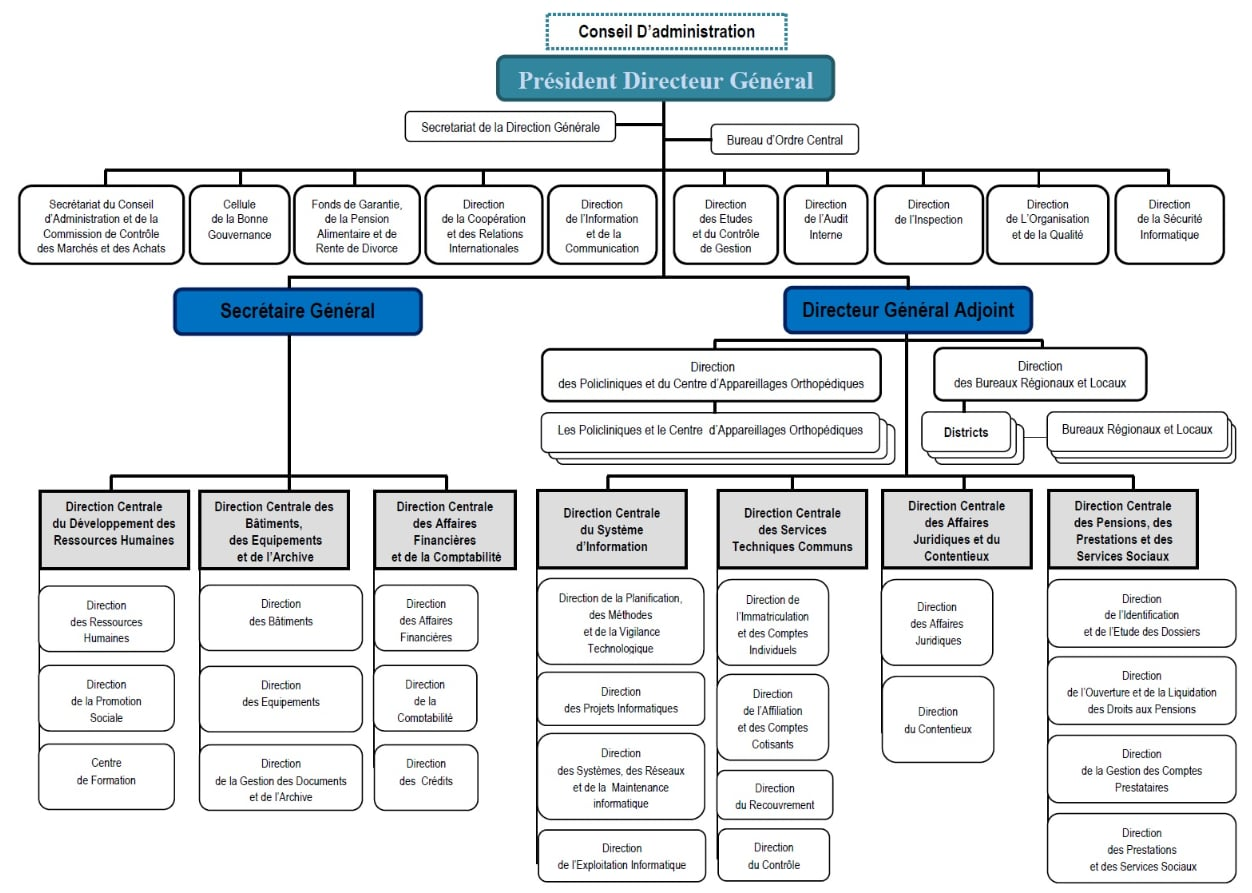
\includegraphics[width=1\textwidth]{figures/orga cnss.jpg} 
    \caption{Organizational Chart of CNSS.}
\end{figure} \ 

\section{Department of Communication and Systems Information (DCSI)}  
The DCSI (Direction de la Communication et des Systèmes d'Information) is a key department within the CNSS Tunisia, responsible for IT systems, digital transformation, and communication strategies.

\subsection{Main Responsibilities}
\begin{itemize}
    \item Information Systems Management (IT Infrastructure).
    \item Maintains and develops the CNSS's digital platforms (e.g., online services for contributors, employers, and beneficiaries).
    \item Ensures data security and system reliability.
    \item Implements new technologies (e.g., AI, cloud computing) for improved service delivery.
\end{itemize}

\subsection{Digital Transformation and E-Services}
\begin{itemize}
    \item Manages the CNSS portal (www.cnss.tn) for online declarations, payments, and claims.
    \item Develops mobile apps (if applicable) for easier access to services.
    \item Works on automating processes (e.g., electronic document management).
\end{itemize}
\subsection{Internal and External Communication}
\begin{itemize}
    \item Handles press relations, media announcements, and public awareness campaigns.
    \item Manages internal communication (employee newsletters, intranet updates).
    \item Organizes training sessions on digital tools for staff and users.
\end{itemize}
\subsection{Cybersecurity and Data Protection}
\begin{itemize}
    \item Implements security protocols to protect sensitive contributor data.
    \item Ensures compliance with Tunisia’s data privacy laws.
\end{itemize}

\subsection{Collaboration with Other Departments}
\begin{itemize}
    \item Works closely with Direction des Prestations (Benefits) to improve online claim processing.
    \item Supports Direction des Collectes (Contributions) in digital payment solutions.
    \item Assists regional offices in IT troubleshooting and system updates.
\end{itemize}
\subsection{ Missions and Values of DCSI} 
\begin{itemize}
    \item Improves efficiency by reducing paperwork and manual processes.
    \item Enhances transparency in social security management.
    \item Ensures secure and modernized services for employers, employees, and retirees.
\end{itemize}

\section{Project Context Description}
\subsection{Project Description}
The Online Folder Management Platform is a web-based system designed to streamline and digitalize the handling of administrative and social security-related documents within the "Caisse Nationale de Sécurité Sociale (CNSS)". The platform aims to enhance efficiency, accessibility, and security by allowing users to manage, track, and retrieve digital folders in a structured manner.
The application is designed to benefit various users, including the Insured , File manager, Office Supervisor, Central Agent and the Central Manager. 

\subsection{Key Functionalities}
\subsubsection{ Folder Creation and Management}
\begin{itemize}
    \item Allows users to create and register new folders (e.g., employee records, pension applications, medical claims).
    \item Supports document uploads in various formats (PDF, images, etc.).
    \item Enables folder categorization based on predefined criteria (e.g., type of request, department, status).
\end{itemize}

\subsubsection{ Advanced Search and Filtering}
\begin{itemize}
    \item Implements a powerful search engine to locate specific folders using keywords, contributor numbers, or document types.
    \item Provides filtering options based on status (pending, approved, rejected), date of submission, and assigned department.
\end{itemize}

\subsubsection{ Workflow and Status Tracking}
\begin{itemize}
    \item Tracks the progress of each request (e.g., under review, awaiting approval, completed).
    \item Notifies users about status updates via email or dashboard alerts.
\end{itemize}

\subsubsection{ Role-Based Access Control (RBAC)}
Defines different access levels for CNSS employees, ensuring data security and compliance.
\begin{itemize}
    \item \textbf{Insured:} Can submit and track their folders.
    \item \textbf{File Manger ,Office Supervisor ,Central Agent:} Can review and process documents also escalate folders to the higher authority when it needs to.
    \item \textbf{Central Manager:} Manage user roles and system configurations.
    
\end{itemize}
\subsubsection{ Integration with CNSS Systems}
\begin{itemize}
    \item Connects with existing CNSS databases to retrieve or verify contributor information.
    \item Supports integration with CNSS’s e-services for automated validation and cross-checking.
\end{itemize}

\subsubsection{ Secure Data Storage}
Implements encryption and secure authentication to protect sensitive data.
\subsubsection{ Analytics and Reporting}
\begin{itemize}
    \item Generates reports on folder processing times, workload distribution, and approval rates.
    \item Provides insights for optimizing workflows within CNSS.
\end{itemize}


\section{Existing System Description}
The current document processing system at CNSS is entirely paper-based, following a traditional workflow with manual intervention at each stage. While documents are eventually scanned and stored in the Electronic Document Management (GED) system, the overall process remains inefficient due to heavy reliance on physical paperwork.
\subsection{Breakdown of the Existing Process}
\textbf{ Step 1: Submission of the Folder by the Insured Person}
\begin{itemize}
    \item The insured person (worker, retiree, or employer) submits a physical folder containing the required documents for a social security-related request (e.g., pension application, medical reimbursement, workplace accident claim).
    \item The folder is manually registered and assigned a reference number by a front-desk agent.
    \item The physical folder is placed in a queue for processing.
\end{itemize}

 \textbf{ Step 2: Processing by the File Manager}
A file manager reviews the submitted folder and checks if all required documents are present.\\
\textbf{Decision Point 1:}
\begin{itemize}
    \item If the folder is complete and meets the requirements, the file manager accepts it and forwards it to the next stage.
    \item If the folder lacks certain documents or contains errors, the file manager rejects it, and the insured person is notified to resubmit.
    \item If the case is complex or requires further review, the file manager escalates it to the Office Supervisor, adding any necessary additional documents.
\end{itemize}

\textbf{ Step 3: Review by the Office Supervisor}
The Office Supervisor handles cases that were escalated by the file manager.
The supervisor performs a secondary review of the folder and can also request additional documents if needed.
\textbf{Decision Point 2:}
\begin{itemize}
    \item If the case is clear and acceptable, the supervisor approves it and forwards it for further processing.
    \item If the case is still unclear or requires higher-level validation, the supervisor escalates it to the Central Agent, attaching any necessary additional documents.
\end{itemize}
 \textbf{ Step 4: Final Decision by the Central Agent}
\begin{itemize}
    \item The Central Agent is the highest authority in the document validation hierarchy.
    \item The agent reviews all escalated cases from the Office Supervisor and makes the final decision.
    \item The agent also has the authority to request further supporting documents from the applicant or the previous levels if needed.
\end{itemize}
\textbf{Decision Point 3:}
\begin{itemize}
    \item If the case is approved, it is finalized and recorded in the CNSS system.
    \item If the case is rejected, the insured person is notified of the reason.
\end{itemize}

\textbf{ Step 5: Document Scanning and Archiving in GED}\\
Once the decision is made, the physical documents are scanned and stored in the Electronic Document Management (GED) system for digital archiving.\\
However, this does not replace the paper documents, which are still physically stored in archives.
\clearpage
\begin{figure}[h]
    \centering
    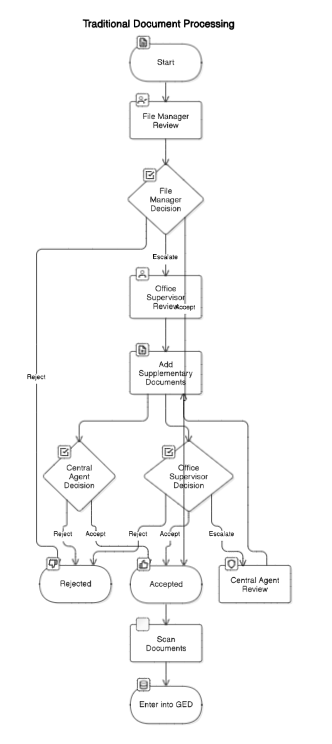
\includegraphics[width=0.5\textwidth]{figures/etude de l'existant.png} 
    \caption{Existing workflow.}
\end{figure} \

\subsection{Critique of the Existing System}
The present system has several inefficiencies and problems:\\
\textbf{ Time-Consuming Process:}
\begin{itemize}
    \item Manual processing of paper-based documents creates delays at every stage.
    \item Cases with multiple escalations take even longer to close.
\end{itemize}

\textbf{ High Risk of Errors and Document Loss:}
\begin{itemize}
    \item Paper-based records are prone to being lost easily, photocopied, and human errors result in loss.
    \item Missing documents make the insured persons physically come again to resubmit documents, resulting in further delays.
\end{itemize}

\textbf{ Limited Tracking and Transparency:}
\begin{itemize}
    \item Applicants have no real-time tracking on the status of their request.
    \item Employees are required to look for files manually, and this generates inefficiencies.
\end{itemize}

\textbf{ Redundant Workload:}
\begin{itemize}
    \item Employees of different levels manually read and process the same documents multiple times.
    \item Scanning documents into GED at the last stage of the process offers an extra step instead of being integrated from the beginning.
\end{itemize}

\textbf{ Physical Storage and Security Issues:}
\begin{itemize}
    \item Paper documents occupy huge storage space, and accessing documents is made inconvenient.
    \item Sensitive documents are prone to destruction (fire, water) or unauthorized access.
\end{itemize}

\subsection{Proposed Solution: Online Folder Management Platform}
The Online Folder Management Platform aims to computerize and streamline the entire process, eliminating the drawbacks of the traditional system. The key Improvements Introduced by the Platform:
\clearpage
\textbf{ Entirely Digital Folder Submission}
\begin{itemize}
    \item Insured clients upload their applications online, with no need for physical visits.
    \item Documents are uploaded and pre-checked for completeness before submission.
\end{itemize}

 \textbf{ Automated Workflow and Tracking}
\begin{itemize}
    \item Each folder is electronically assigned to the respective file manager, office supervisor, or central agent.
    \item Users can view the status of their request in real-time using an online portal.
\end{itemize}

\textbf{ Role-Based Access and Automated Escalations}
\begin{itemize}
    \item Cases are automatically escalated to the appropriate level based on predefined rules by the system.
    \item Supervisors and agents are immediately alerted to pending work.
\end{itemize}

 \textbf{ Advanced Search and Document Management}
\begin{itemize}
    \item Digital files are searchable instantly using an advanced filtering system.
    \item No risk of document loss as all documents are stored securely in a centralized repository. 
\end{itemize}

\textbf{ Integration with GED Made Easy}
\begin{itemize}
\item Documents are stored directly in GED upon submission, eliminating duplicate scanning processes.
\item Compliance with data security policy and access controls is guaranteed by the system.
\end{itemize}

 \textbf{ Efficiency Improvement and Cost Reduction}
\begin{itemize}
    \item Eliminating paper-based workflows saves operational costs and manual labor.
    \item Reduced processing time translates to improved service quality for the insured.
\end{itemize}

\section{Language and Design Methodology}

To implement a programming project in a group environment is to master key development methodologies in order to obtain the best and structured lifecycle.
In an effort to formally formalize the solution outlined, it is essential to invoke a shared modeling language. This is useful in establishing a basic and abstract perception of the project through the enforcement of standardized concepts and rules.
Depending on the nature of the project, teams may adopt either traditional methodologies or agile methodologies.

\subsection{ Agile Methodologies}
\textbf{"Agile development is a software development approach that emphasizes iterative and incremental processes, focusing on customer satisfaction, teamwork, and adaptability to changing requirements throughout the project." \cite{somebook}}\\
This approach accelerates software development by first offering a minimum viable version and then incrementally adding features in iterative loops.
Agile methodology is a more recent approach that improves productivity, reduces development costs, and provides greater visibility into project management.
\begin{figure}[h]
    \centering
    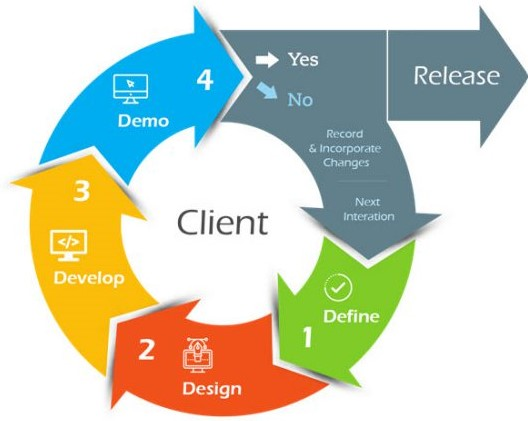
\includegraphics[width=0.5\textwidth]{figures/agile.jpg} 
    \caption{Agile Methodology.}
\end{figure}\
\clearpage

\subsection{Keys and advantages of Agile Methodology}
\begin{table}[h]
\centering
\begin{tabular}{|c|l|}
\hline
\textbf{No.} & \textbf{Principle} \\ \hline
1  & Satisfy the customer early and continuous delivery. \\ \hline
2  & Encourage changing requirements during collaboration with the customer. \\ \hline
3  & Focus on frequent delivery from the very start of the project. \\ \hline
4  & Ensure cooperation between the project team and business people. \\ \hline
5  & Build projects around a motivated team. \\ \hline
6  & Foster direct dialogue. \\ \hline
7  & Measure project progress based on the operational functionality of the product. \\ \hline
8  & Adopt a sustainable and constant development rhythm for all project participants. \\ \hline
9  & Continuously control technical excellence and good design. \\ \hline
10 & Minimize unnecessary work. \\ \hline
11 & Self-organize and empower teams. \\ \hline
12 & Fine-tune the process by making use of project management tools. \\ \hline
\end{tabular}
\caption{Principles of Agile and Scrum}
\end{table}

\subsection{Common Agile Methods}
When an organization is looking to apply Agile development management, it is still necessary to choose the most suitable method for its project. The reason behind this is that Agile methods themselves are numerous, and they are a source of confusion. Among the most widely known Agile methods currently in use, there are:
\begin{itemize}
    \item eXtreme Programming (XP).
    \item Scrum.
    \item Feature Driven Development (FDD).
    \item Lean Software Development.
    \item Agile Unified Process (Agile UP or AUP).
    \item Crystal.
    \item Dynamic Systems Development Method (DSDM).
\end{itemize}
\begin{figure}[h]
    \centering
    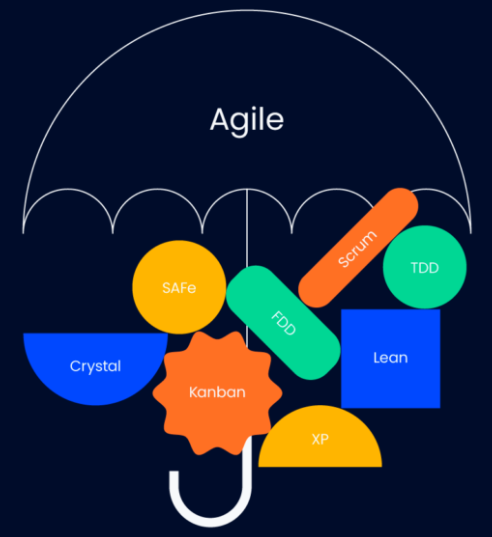
\includegraphics[width=0.7\textwidth]{figures/agileUmbrella.png}  % Replace with your image file
    \caption{SCRUM Ceremonies.}
    \label{fig:image1}
\end{figure} \ 
\clearpage

\section{SCRUM}
\textbf{"Scrum is an agile project management framework that helps teams structure and manage their work through a set of values, principles, and practices. Much like a rugby team (where it gets its name) training for the big game, scrum encourages teams to learn through experiences, self-organize while working on a problem, and reflect on their wins and losses to continuously improve."}\cite{samplewebs1}\\
Scrum principle entails using various processes and techniques to control the creation of complex products with a view to improving and guiding their progress.
Scrum development cycles are based on a series of iterations, or sprints, that are short in duration (typically two to four weeks).
\begin{figure}[h]
    \centering
    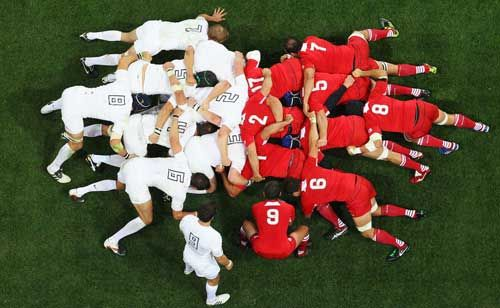
\includegraphics[width=0.7\textwidth]{figures/rugbystock.jpg} 
    \caption{Rugby SCRUM Stock.}
\end{figure} \
\subsection{Why SCRUM}
\textbf{"Scrum is the most popular Agile framework. According to 'Digita.ai' 16th annual report, 87\% of organizations using an Agile framework use Scrum. That’s up from 58\% of Agile teams using Scrum, as documented in the 14th annual State of Agile report."\cite{samplewebs2}} 
The key benefits of using Scrum are:

\begin{itemize}
    \item Quicker delivery of working product to customers and users
    \item Enhanced quality
    \item Enhanced productivity
    \item Lower costs
    \item Enhanced ability to add changes as and when they occur
    \item Enhanced employee morale
    \item Enhanced user satisfaction
    \item Capability to deliver complex projects which were not feasible earlier
\end{itemize}
\subsection{SCRUM Framework}
This visual shows the iterative nature of Scrum with continuous planning, execution, and improvement:
\begin{figure}[h]
    \centering
    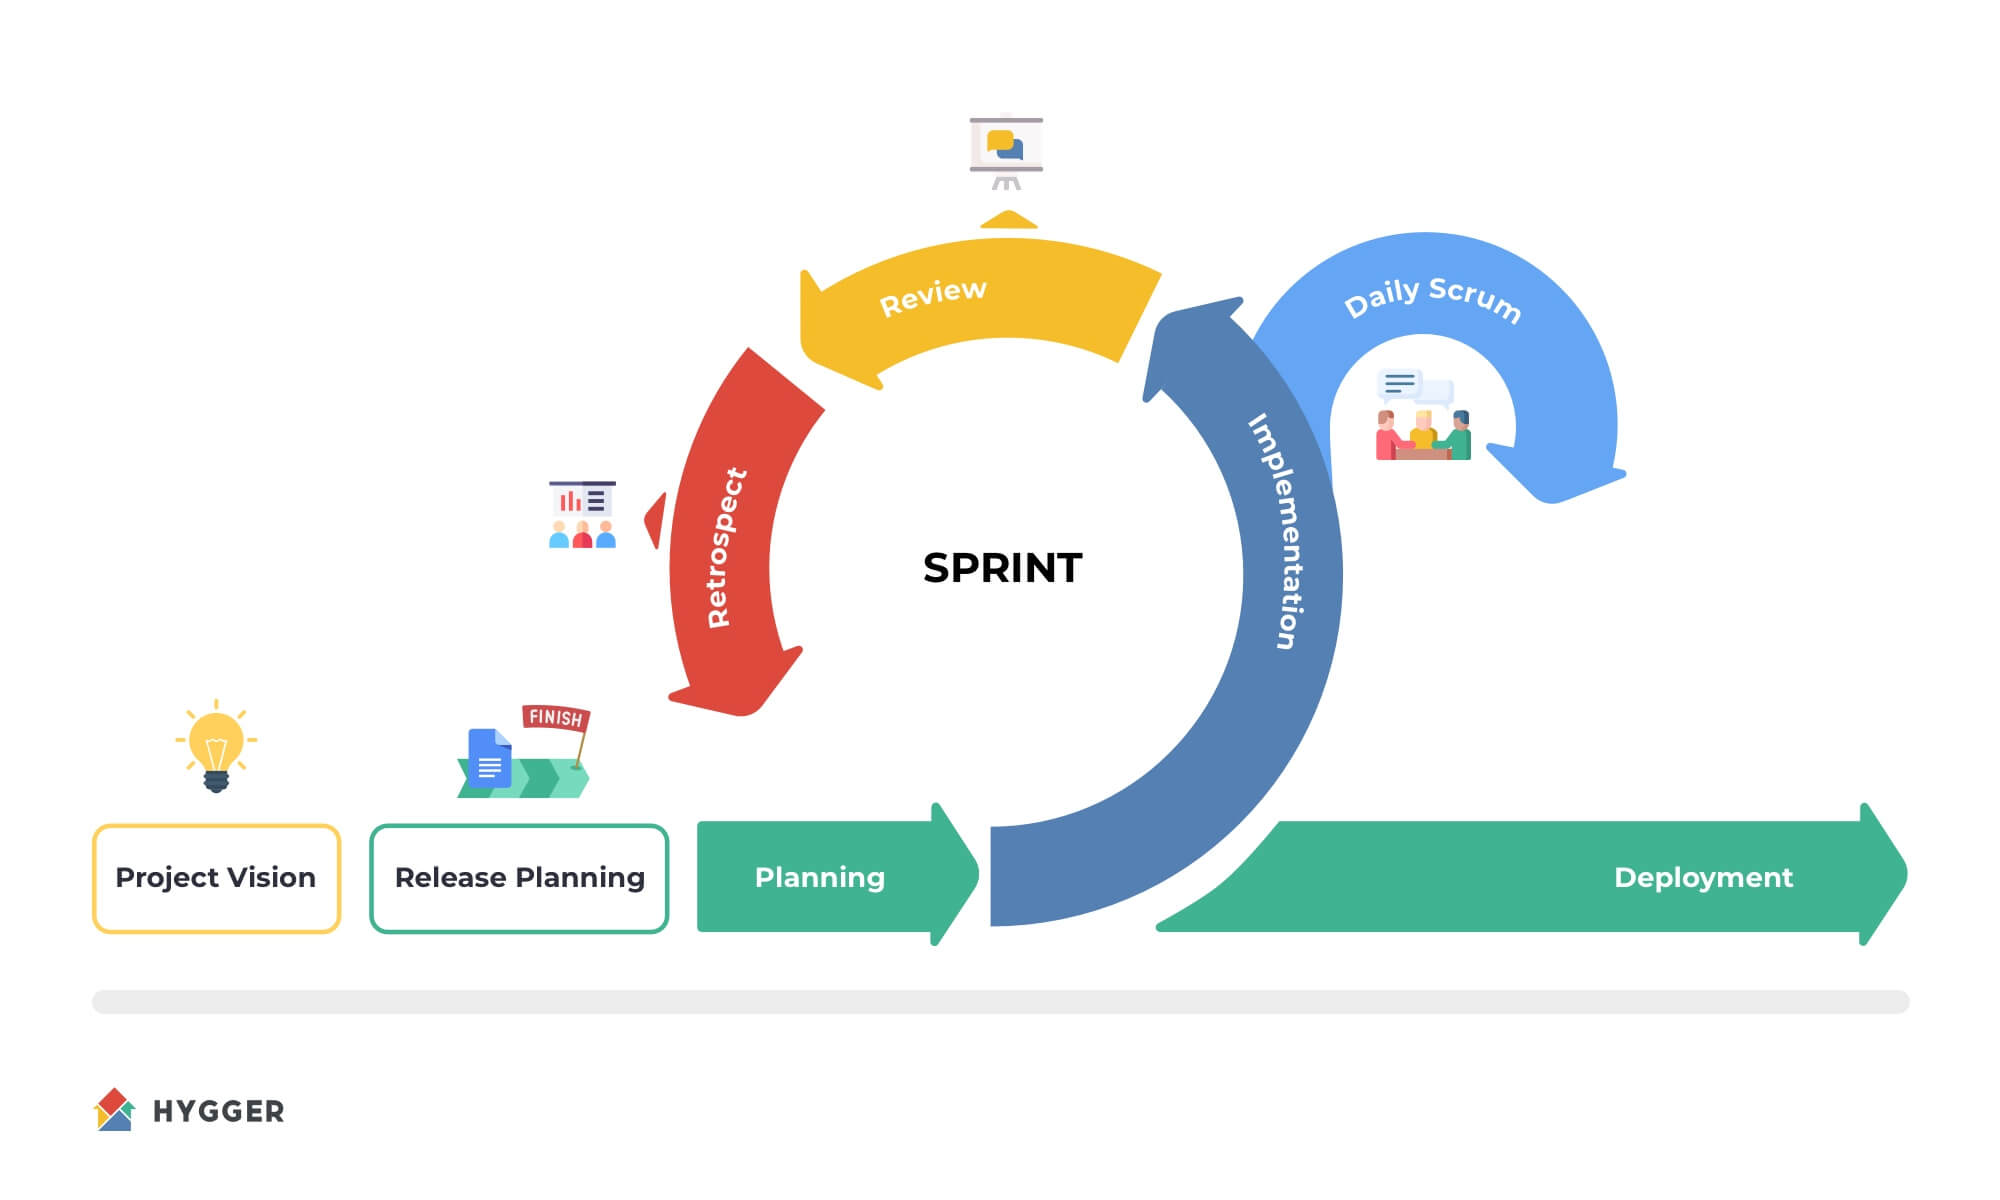
\includegraphics[width=0.7\textwidth]{figures/Sprint-review-table-2-1.jpg} 
    \caption{SCRUM Review table.}
\end{figure} \ 
\begin{enumerate}
    \item \textbf{Project Vision:} Defines the overall purpose and goal of the project.
    \item \textbf{Release Planning:} Identifies key deliverables and timeframes.
    \item \textbf{Planning:} Defines activities and objectives for the upcoming sprint.
    \item \textbf{Implementation:} Development phase where activities are executed.
    \item \textbf{Daily Scrum:} Short daily meetings to track progress and fix issues.
    \item \textbf{Review:} Inspection of work completed, gathering feedback.
    \item \textbf{Retrospect:} Inspection of the sprint for improving future performance.
    \item \textbf{Deployment:} Release of finished work into use.
\end{enumerate}
\subsection{SCRUM Team}
\begin{figure}[h]
    \centering
    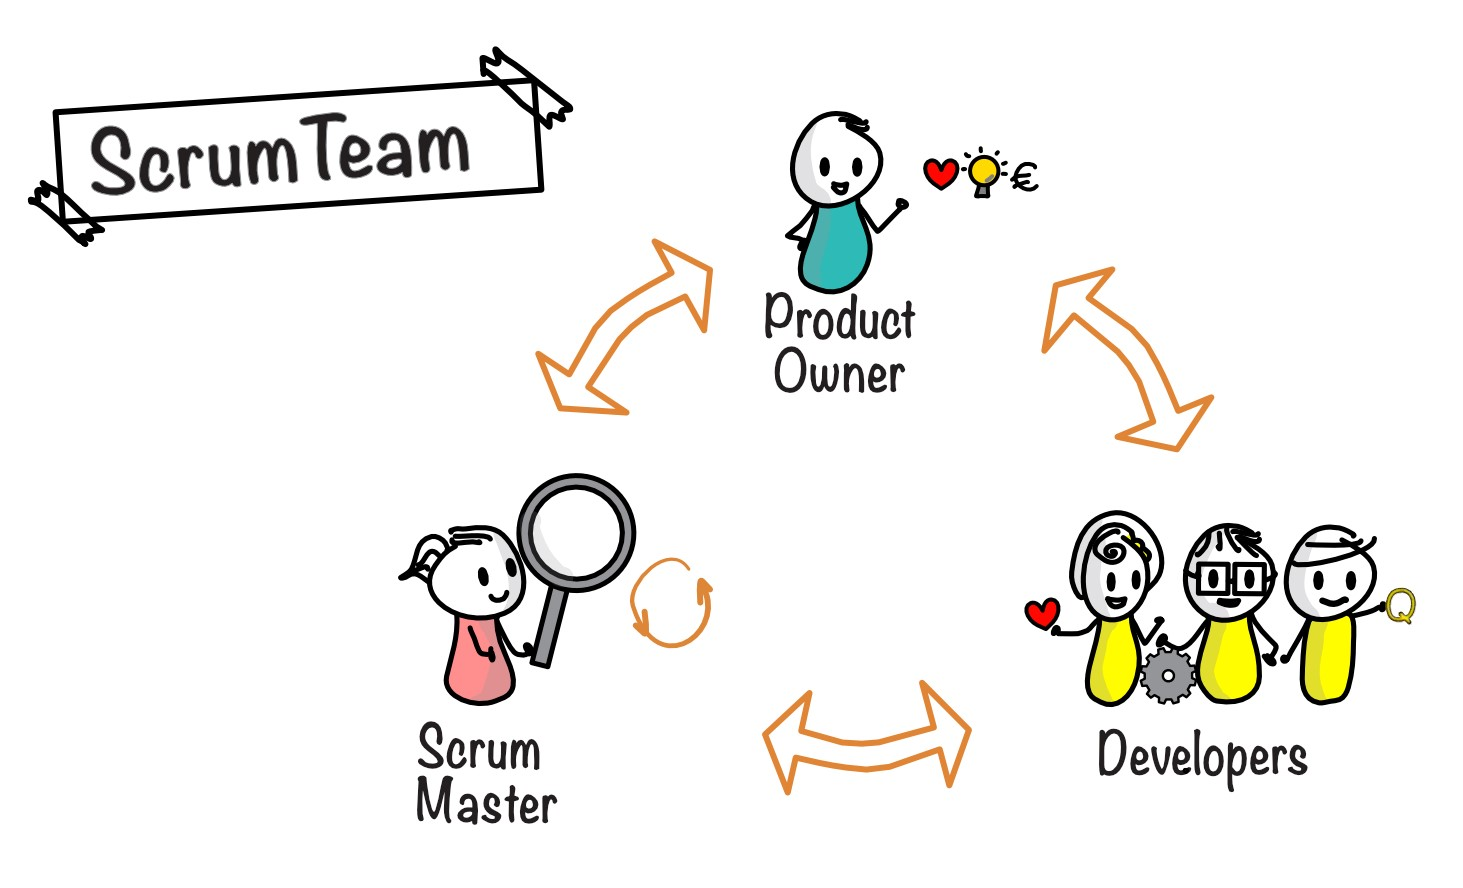
\includegraphics[width=0.7\textwidth]{figures/Scrum Team.png} 
    \caption{SCRUM Team.}
\end{figure} \ 
\textbf{Product Owner:}
\begin{itemize}
    \item Defines the project vision and goals.
    \item Manages the product backlog.
    \item Takes care of business needs.
\end{itemize}
\textbf{Scrum Master:}
\begin{itemize}
    \item Facilitates the Scrum process.
    \item Removes impediments for the team.
    \item Follows Agile principles.
\end{itemize}
\textbf{Developers:} 
\begin{itemize}
    \item Develop and deliver the product.
    \item Collaborate to deliver features.
    \item Participate in sprint activity.
\end{itemize}
\subsection{Artifacts in SCRUM}
\begin{itemize}
    \item \textbf{Product Backlog:}A list of features that are expected or required by the client for the product. The document keeps on changing during the project based on the requirement of the client. The product owner updates the product backlog.
    
    \item \textbf{Sprint Backlog:}Is the master plan to achieve the Sprint goal, as defined during the Sprint planning meeting. The team maintains the Sprint backlog to have a good idea about the progress of the remaining work in the Sprint.
    
    \item \textbf{Key Burn Down Chart:}This chart is easy to use and indicates the work to be done in completing the tasks in the Sprint backlog. It displays the work remaining (usually expressed in hours) against time (in days). The Burndown Chart is updated daily by the Scrum Master after the stand-up meeting every day.
\end{itemize}

\subsection{Sprint Activities}
\begin{itemize}
    \item \textbf{Sprint Planning:} A planning and objective setting session for a sprint. The session can last up to eight hours in duration for a four-week Sprint.
    \item \textbf{Daily Stand-up (Daily Scrum):} A 15-minute development team meeting, led by the Scrum Master, which is used to synchronize, track progress, and plan work for the next 24 hours.
    \item \textbf{Iteration Review:} After every sprint, the stakeholders and Scrum team have a meeting with the product owner to ensure the delivered product. This can be as long as four hours for a four-week Sprint.
    \item \textbf{Sprint Retrospective:} A Scrum team internal meeting to figure out what went right and what needs to change. This type of meeting will at most last three hours for a four-week Sprint.
\end{itemize}

\section{UML Modeling Language}
\begin{figure}[h]
    \centering
    
\includegraphics[width=0.5\textwidth]{figures/UML_logo.png} 
    \caption{UML Modeling Language.}
\end{figure} \ 
\textbf{"UML, short for Unified Modeling Language, is a standardized modeling language consisting of an integrated set of diagrams, developed to help system and software developers for specifying, visualizing, constructing, and documenting the artifacts of software systems, as well as for business modeling and other non-software systems." \cite{samplewebs3}}\\
We chose UML as our modeling language to model our application. We used it due to its merits, particularly its standardization and the wealth of diagrams.
In addition, UML is the best tool available for diagramming complex systems in a straightforward and standardized graphical and textual notation.
\newpage
\begin{center}
    \doublespacing 
    \centering
    \LARGE\textbf{Conclusion} 
    \vspace{1cm} \\
    \raggedright
\end{center}
\addcontentsline{toc}{section}{Conclusion} 
We began our report with this first chapter, in which we brushed upon several significant points starting with the host organization's introduction, CNSS.
\vspace{0.5cm}
We then set out the context of our internship by stating the problem and proposing a likely solution to the current state of affairs.
\vspace{0.5cm}
Finally, we have defined our methodological preference and modeling language. From here on, planning and architecture is our concern.

  
\clearpage  
\chapter{Planification And Architecture}
\newpage
\begin{center}
    \doublespacing 
    \centering
    \LARGE\textbf{Introduction} 
     \vspace{1cm} \\
   \raggedright
\end{center}
\Large As outlined in the previous chapter, we have decided to use the Scrum methodology for the design of our platform.  
In this chapter, titled "Planning and Architecture" or "Sprint Zero," we will undertake the initial phase of the Scrum approach. This involves defining user roles, identifying functional and non-functional requirements, and compiling them into a product backlog.

\section{Requirements Specification}
To successfully achieve the desired goals, it is important to frame the project properly by aligning it with the necessary requirements and a well-thought-out plan.
\subsection{Actors Identification}
\Large Here’s a structured and humanized description of each actor and their role, showing how responsibilities escalate through the hierarchy:   

\subsubsection{Insured}
The insured person is the primary user of the platform. They can: 
\begin{itemize}
    \item  Submit requests through dynamic forms.
    \item  Track the status of their submissions.
    \item  Manage their personal profile.
\end{itemize}
Once they submit a request, it enters the system, where different actors handle and review it.  

\subsubsection{Submission Coordinators}  
This level includes two key roles responsible for processing submissions before they reach higher authorities:  

\textbf{- File Manager:}\\
\begin{itemize}
    \item  Reviews submitted requests to ensure they are complete and accurate.
    \item  If necessary, forwards submissions for further processing.
\end{itemize}

\textbf{- Office Supervisor: } 
\begin{itemize}
    \item  Oversees the submission process within an office.
    \item  Tracks workflows and ensures smooth operations.
    \item  Views office and basic statistics to monitor performance.
\end{itemize}


\subsubsection{ Central Agent} 
\begin{itemize}
    \item  Manages both "File Managers" and "Office Supervisors" to ensure efficient processing.
    \item  Ensures proper coordination and treatment of the files that have been escalated to him.
\end{itemize}

\subsubsection{ Central Manager } 
\begin{itemize}
    \item  Holds the highest authority in the system.
    \item  Publishes important news and updates on the platform.
    \item  Monitors global statistics to track overall performance.
    \item  Ensures system-wide efficiency.
    \item  Authenticates users and ensures security.
\end{itemize}

\subsection{Escalation Flow}  
\begin{enumerate}
    \item Insured submits a request.
    \item Submission Coordinators (File Manager and Office Supervisor) review and process it. If necessary, they escalate to the Central Agent for higher-level management.
    \item The "Central Agent" ensures proper handling.
\end{enumerate}
This hierarchy ensures an organized workflow, with responsibilities clearly defined at each level.
\subsection{Static Context Diagram}
A static context diagram helps determine how the system relates to the actors and establishes how many instances of the different actors exist at one point in time to the system.
\begin{figure}[h]
    \centering
    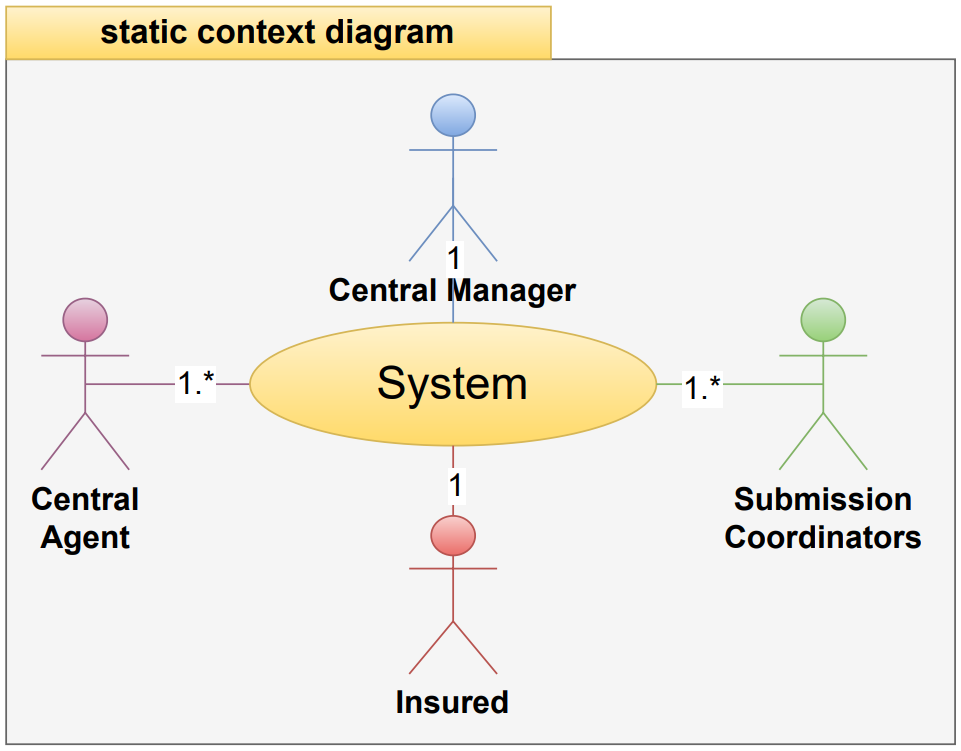
\includegraphics[width=0.6\textwidth]{figures/statdia.png}
    \caption{Static context Diagram.}
\end{figure} \ 
\subsection{Identification of Functional Requirements}
Functional requirements or use cases from the perspective of UML can be described as follows: \textbf{"A use case explains how users interact with a product or system. It outlines the flow of user inputs, establishing successful and failed paths to meeting goals."}\cite{samplewebs4}\\
Functional requirements define the functionalities of the system that are made available to different actors to satisfy their needs and expectations.
Each of the functional requirements is a list of steps executed by our system in order to react to an application's request.
\begin{enumerate}
    \item Insured

     \begin{itemize}
         \item Submit requests through dynamic forms.
         \item Track the status of submissions (e.g., pending, approved, rejected).
         \item View notifications (approvals, rejections).
         \item Alerts for submissions.
         \item Access news/announcements published on the platform.
         \item Manage profile (update personal details).
     \end{itemize}
 
\item File Manager
\begin{itemize}
    \item Review submissions according to his actual region.
    \item Escalate further files to the Office Supervisor + adds additional documents if needed.
    \item Access basic statistics.
\end{itemize}
    
\item Office Supervisor
\begin{itemize}
    \item Review forwarded submissions (from File Managers).
    \item Supervise assigned File managers (review their work).
    \item Escalate to Central Agent  + adds additional documents if needed.
    \item Access basic statistics.
\end{itemize}
    
\item Central Agent
\begin{itemize}
    \item Manage File Managers and Office Supervisors (create accounts, assign roles).
    \item Review submissions forwarded from the Office supervisors.
    \item View basic statistics.
    \item Review the office supervisors work.
\end{itemize}

\item Central Manager
\begin{itemize}
    \item Publish platform news/updates.
    \item Configure dynamic forms (customize fields).
    \item Manage internal stakeholders.
    \item Tracks the flow of every submissions process.
    \item View global statistics.
\end{itemize}
    
\item System (Automated Functions)

\begin{itemize}
    \item Authenticate users (secure login, role-based access).
    \item Send automated emails (notifications, status updates).
    \item Validate national identity documents and extract important data.
    \item Generate automated statistics.
\end{itemize}
\end{enumerate}
\subsection{Identification of Non-Functional Requirements}
At some stage in the project life, the team has to consider non-functional requirements. These are requirements that lie within the system and are invisible to the end-user. The platform has to satisfy the following conditions:

\begin{itemize}
    \item \textbf{Performance:} Also known as response time, is a growing concern. There is a need to optimize our platform's page loading times.

\item \textbf{Accessibility:} Our website is at the core of the Information System Department operations, and therefore it is critical that it is operational at all times.

\item \textbf{Usability:} The interfaces must be easy to use and not complicated by adhering to usability guidelines.
  
\item \textbf{Security:} Since the application is filled with personal information, the access to different parts must be protected through passwords and access privileges.
  
\item \textbf{Maintainability:} The code must be structured in a readable, well-organized, and clear form to facilitate the maintenance of the various modules of the application.
\item \textbf{Storage:} As our platform deals with a huge quantity of non-structured data therefore we insured that the documents are well archived including relevant meta data for easy retrieval and organisation.
\end{itemize}
\section{ Project Structure and Breakdown}
\subsection{Identification of the SCRUM Team}
The most critical stakeholder of SCRUM is the SCRUM team.
In our project example, Mr. Oussama Cherif will be the Product Owner because he meets all the requirements to be a Product Owner. Ms. Saoussen Anssi will be the Scrum Master, and we, Nourchene Garbouj and Yassine Ben Yedder, are the Development Team.
\begin{figure}[h]
    \centering
    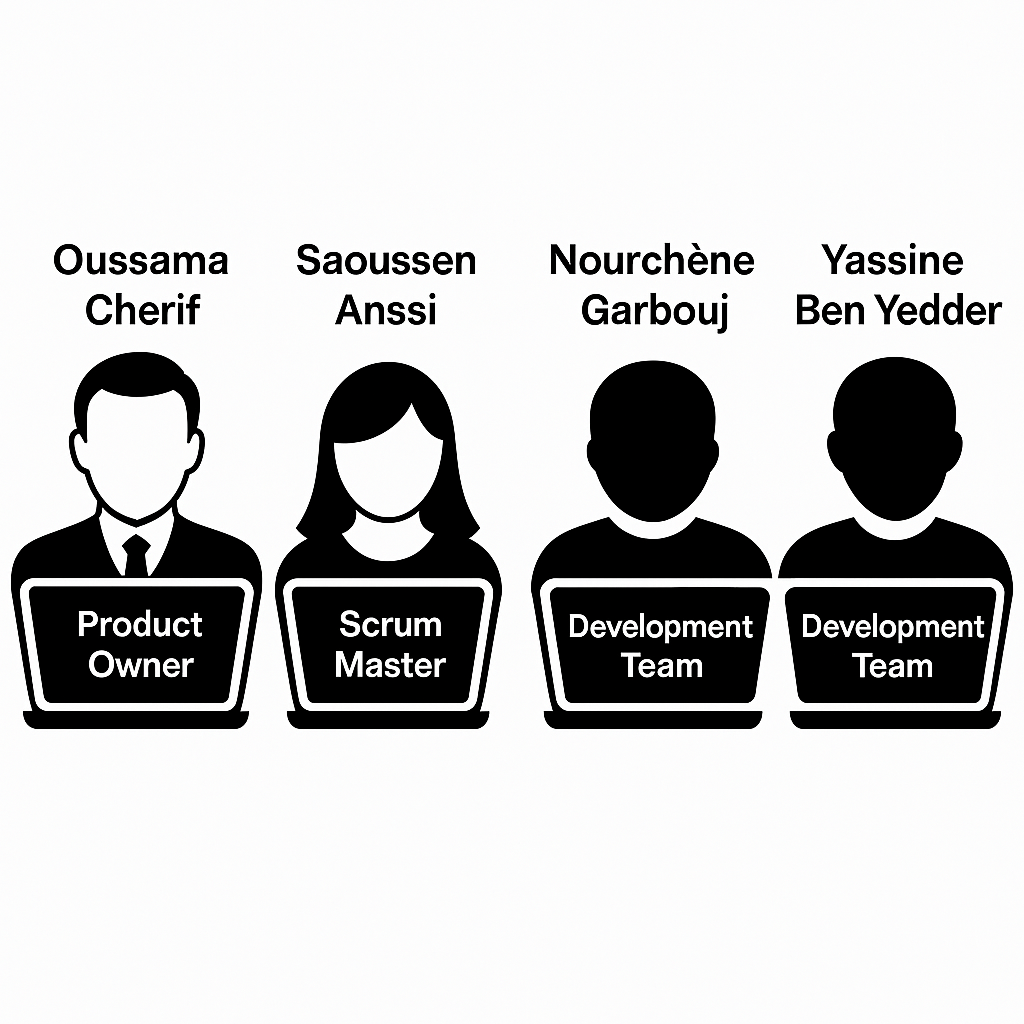
\includegraphics[width=0.7\textwidth]{figures/scrumteam.png} 
    \caption{Roles of the Team.}
\end{figure} \

\subsection{Product Backlog}
As defined in the first chapter, the product backlog is a very important artifact that represents the expected requirements and functionalities.  
We present in Table 2.1 a summary of the product backlog related to our solution, which lists the following fields:

\begin{itemize}
    \item \textbf{ID:} A unique and incremented identifier for each new User Story.
    \item \textbf{User Story:} Describes the content of a functionality.
    \item Description: A short description of the task to be completed, defined as follows: As a <role>, I want to <do something> so that <I can get value>.
    \item \textbf{Priority:} The level of importance assigned to this task by the Product Owner (High or Medium).
    \item S\textbf{tory Points:} are a relative measure of effort used to estimate the complexity, work, and risk of a user story.
\end{itemize}


\newcolumntype{L}[1]{>{\raggedright\arraybackslash}p{#1}}
\begin{longtable}{|c|L{3.5cm}|L{4.4cm}|c|c|}
\hline
\textbf{ID} & \textbf{User Story} & \textbf{Description} & \textbf{Priority} & \textbf{Story Points} \\
\hline
\endfirsthead
\hline

01 & Submit requests via dynamic forms & As an \textbf{Insured}, I want to submit requests through dynamic forms so that my requests can be processed properly. & High & 8 \\
\hline
02 & Validate national ID documents & As a \textbf{System}, I want to validate identity documents so that I can extract reliable user data. & High & 8 \\
\hline
03 & Manage dynamic forms & As a \textbf{Central Manager}, I want to manage dynamic forms so that forms can be customized when needed. & High & 6 \\
\hline
04 & Authenticate & As a \textbf{User}, I want to authenticate so that I can access the platform securely. & High & 5 \\
\hline
05 & Review submission & As a \textbf{Submission Coordinator}, I want to review submissions so that I ensure their correctness. & High & 5 \\
\hline
06 & Review forwarded submissions & As a \textbf{Central Agent}, I want to review forwarded submissions so that I can validate them centrally. & High & 5 \\
\hline
07 & Manage user roles & As a \textbf{Central Agent}, I want to manage File Managers and Office Supervisors so that I ensure proper workflow. & High & 5 \\
\hline
08 & Track submission workflows & As a \textbf{Central Manager}, I want to track workflows so that I can monitor overall submission health. & High & 6 \\
\hline
09 & Reset forgotten password & As an \textbf{Insured}, I want to reset my password so that I can regain access to my account. & High & 3 \\
\hline
10 & Track submission status & As an \textbf{Insured}, I want to track the status of my requests so that I stay informed about their progress. & Medium & 5 \\
\hline
11 & Manage profile & As a \textbf{User}, I want to manage my profile so that my personal information stays up to date. & Medium & 3 \\
\hline
12 & View basic statistics & As a \textbf{Submission Coordinator}, I want to view basic statistics so that I can analyze performance. & Medium & 3 \\
\hline
13 & Consult notifications & As an \textbf{Insured}, I want to consult notifications so that I don’t miss important updates. & Medium & 3 \\
\hline
14 & Monitor office supervisors & As a \textbf{Central Agent}, I want to monitor office supervisors so that I ensure their tasks are progressing. & Medium & 4 \\
\hline
15 & Monitor file managers & As an \textbf{Office Supervisor}, I want to monitor file managers so that I can supervise their work. & Medium & 4 \\
\hline
16 & View global statistics & As a \textbf{Central Manager}, I want to view global statistics so that I can evaluate platform performance. & Medium & 4 \\
\hline
17 & Manage internal stakeholders & As a \textbf{Central Manager}, I want to manage stakeholders so that I can ensure project alignment. & Medium & 5 \\
\hline
18 & Receive submission emails & As an \textbf{Insured}, I want to receive email notifications so that I am alerted about any updates on my submissions. & Medium & 2 \\
\hline
19 & See platform news & As an \textbf{Insured}, I want to see the news so that I stay informed about platform announcements. & Medium & 2 \\
\hline
20 & Publish news & As a \textbf{Central Manager}, I want to publish news on the platform so that users are informed. & Medium & 2 \\
\hline
\caption{Product Backlog Table}
\end{longtable}

\subsection{SCRUM Tool}
Jira is a powerful project management tool designed to support Agile and Scrum methodologies. It allows teams to plan and manage sprints, track tasks through customizable boards, and organize product backlogs efficiently. With features like real-time collaboration, workflow automation, and detailed reporting, Jira enhances team visibility and productivity. It also supports Scrum ceremonies such as sprint planning, reviews, and retrospectives, promoting continuous improvement throughout the development cycle.
\begin{figure}[h]
    \centering
    
\includegraphics[width=0.6\textwidth]{figures/jira logo.png} 
    \caption{Roles of the Team.}
\end{figure} \

\subsection{Sprint Structure}
\subsubsection{Project Sprint Planning}
The sprint planning phase is vital to the successful execution of a project. It provides for the best approach to task decomposition and allocation based on priorities, time, and team capacity, in order to be able to meet the requirements laid out by the Product Owner better.\\
\textbf{"Sprints are time-constrained periods of one week to one month, during which a product owner, Scrum master and Scrum team work to complete a specific product addition. During a sprint, work is done to create new features based on the user stories and backlog."}\cite{samplewebs5}
\begin{figure}[h]
    \centering
    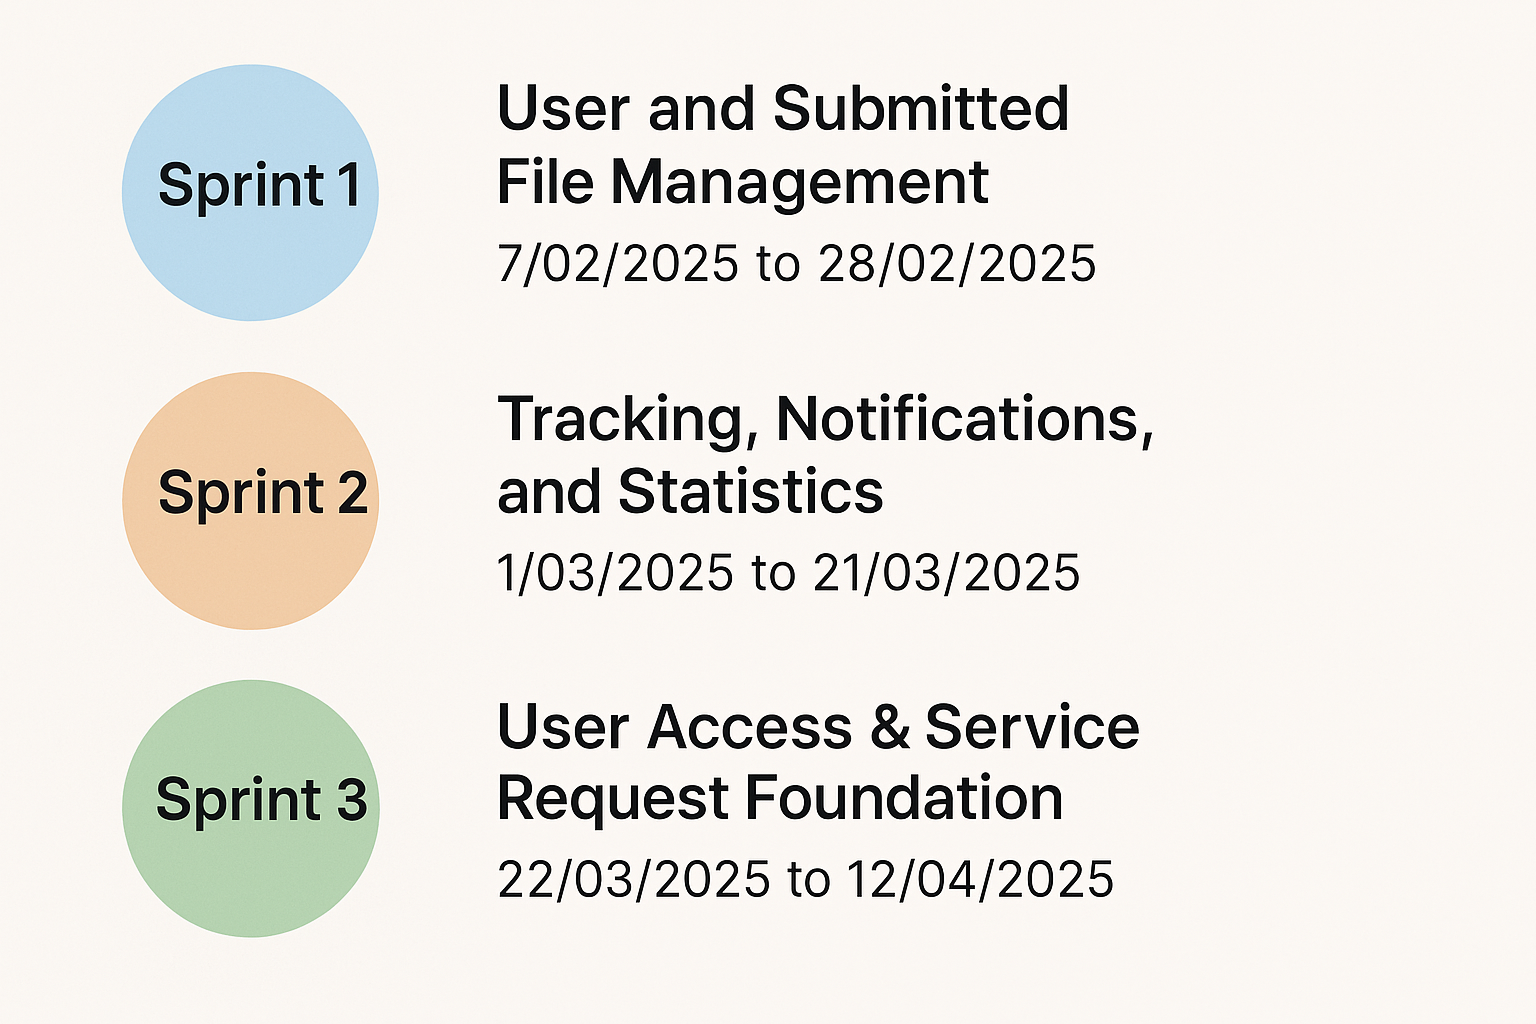
\includegraphics[width=0.5\textwidth]{figures/sprints.png}  
    \caption{Sprints Planification.}
\end{figure} \
\subsection{Project execution plan}
\begin{figure}[h]
    \centering
    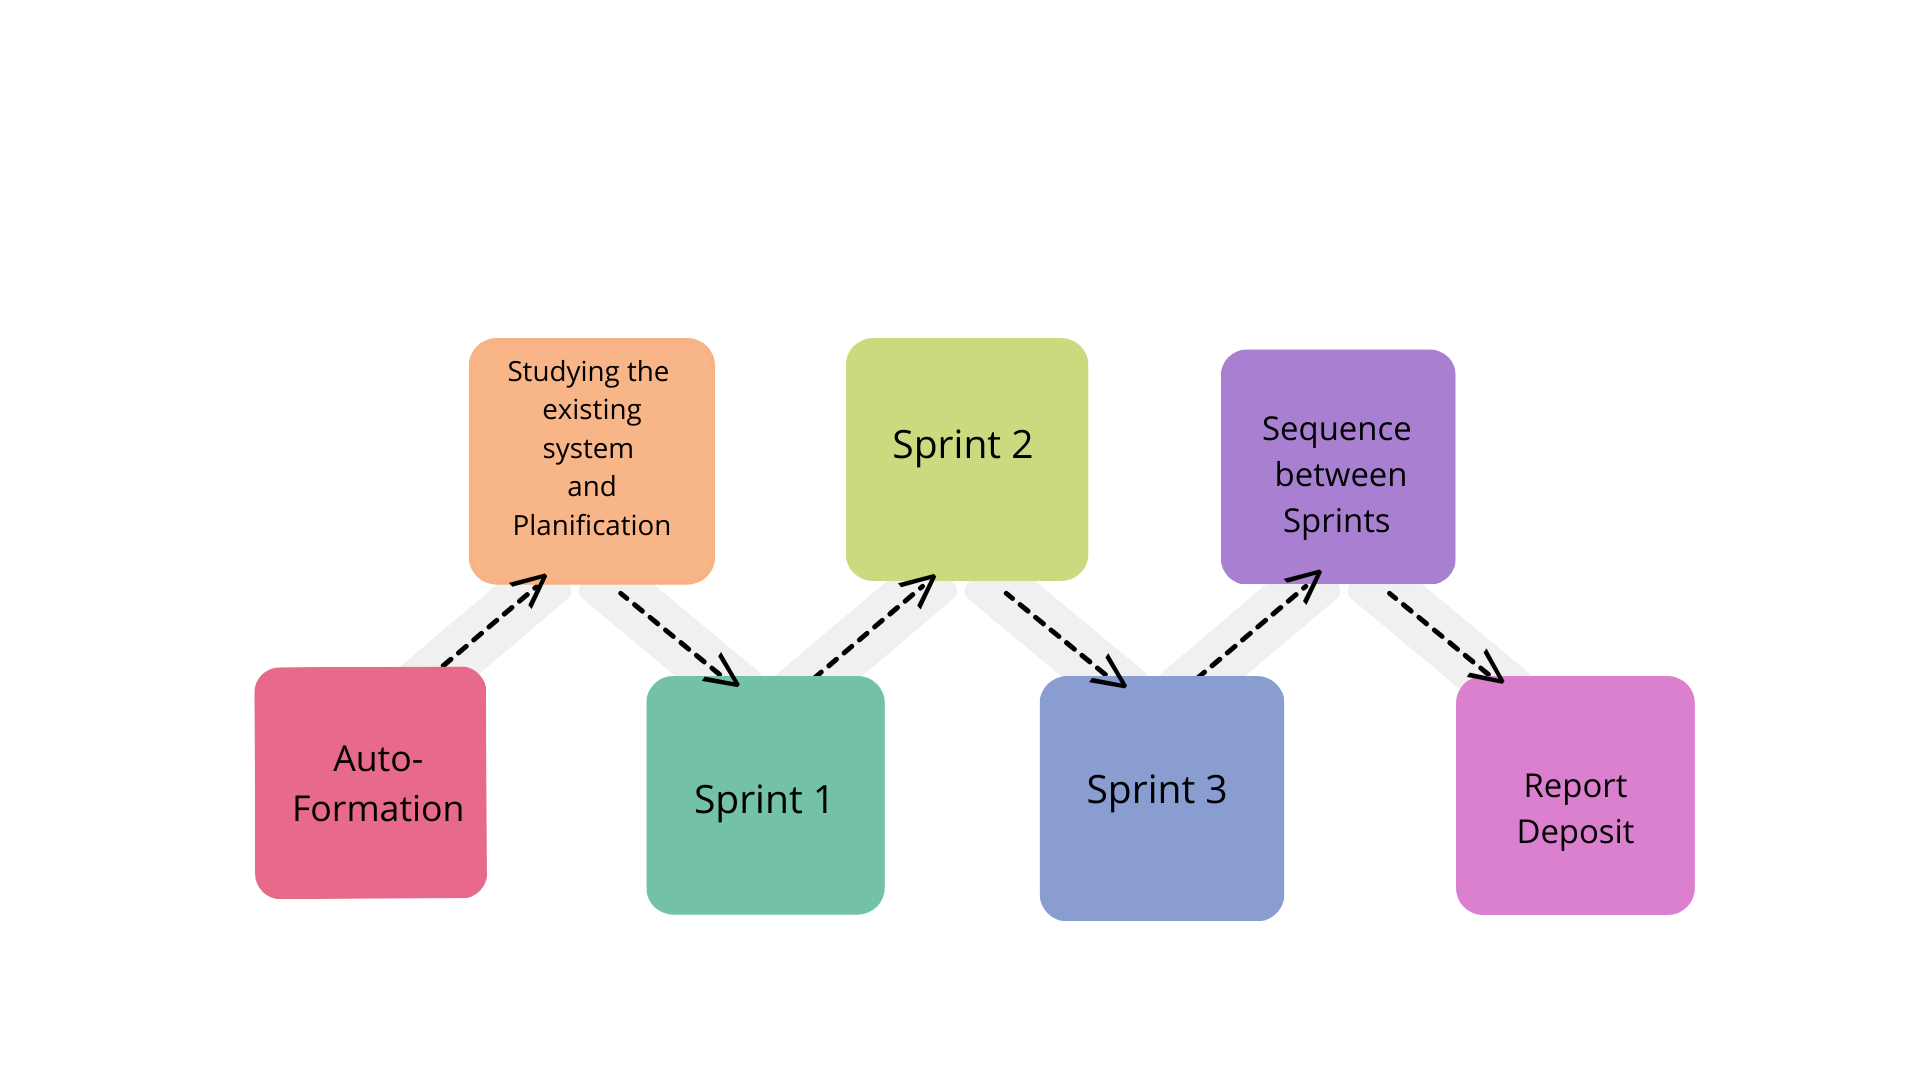
\includegraphics[width=1\textwidth]{figures/sprintplan.png} 
    \caption{Execution Plan.}
\end{figure} \
\clearpage
\begin{itemize}
    \item \textbf{15/01/2025 - 31/01/2025:} Auto-Formation.
    \item \textbf{01/02/2025 - 07/02/2025:} Studying the existing system and planification.
    \item \textbf{07/02/2025 - 28/02/2025:} Sprint 1.
    \item \textbf{01/03/2025 - 21/03/2025:} Sprint 2.
    \item \textbf{22/03/2025 - 12/04/2025:} Sprint 3.
    \item \textbf{13/04/2025 - 30/04/2025:} Sequence between Sprints.
    \item \textbf{22/05/2025}: Report deposit.
\end{itemize}
\clearpage

\section{Global Use Case Diagram}
\begin{figure}[h]
    \centering
    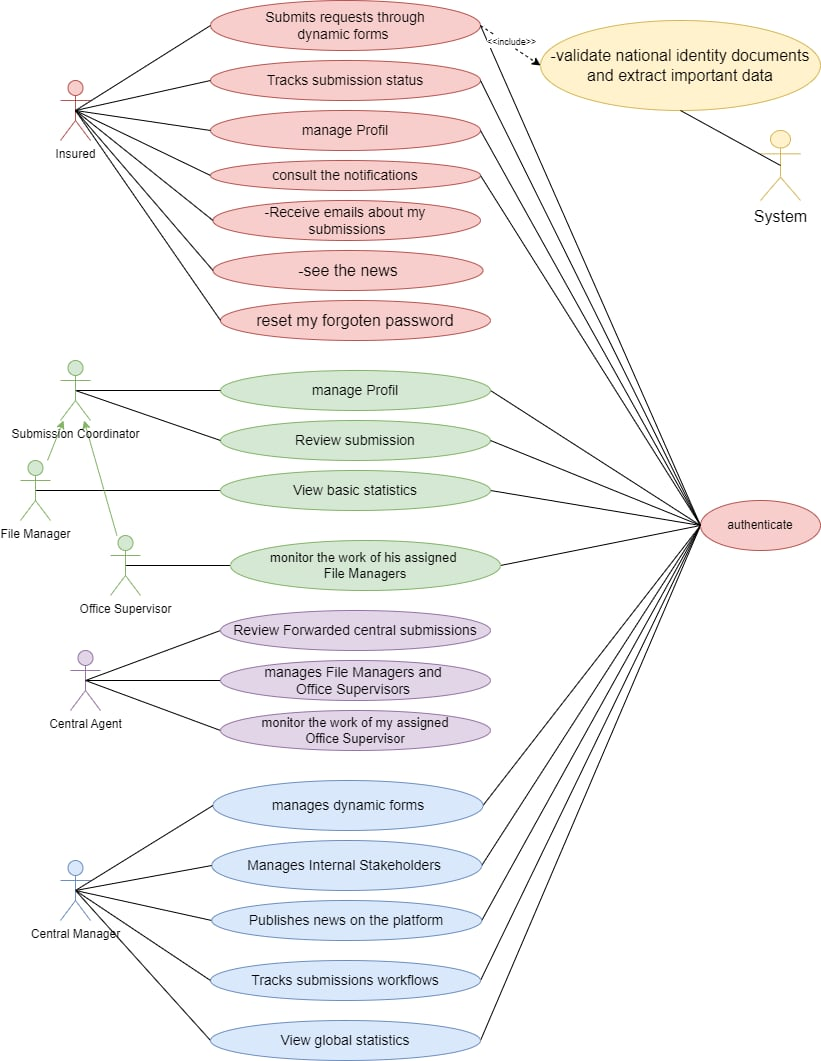
\includegraphics[width=0.9\textwidth]{figures/usecaseglobal.jpg} 
    \caption{Global Use Case Diagram.}
\end{figure} \

\clearpage
\begin{center}
    \doublespacing
    \centering
    \LARGE\textbf{Conclusion} 
    \vspace{1cm} \\
    \raggedright
\end{center}
\addcontentsline{toc}{section}{Conclusion}
In this chapter, we defined the stakeholders and outlined the product backlog based on the identification of both functional and non-functional requirements of our project.
\vspace{0.5cm}
Next, we took the first step toward Scrum by identifying the team, the product backlog, and the sprints. Finally, we created the overall use case diagram for our project.
\vspace{0.5cm}
In the next chapter, we will move on to our first sprint, which ultimately represents a potentially deliverable first version.


  
\clearpage 
\chapter{Sprint 1:  User and Submitted File Management}
\newpage
\begin{center}
    \centering
    \LARGE\textbf{Introduction} 
     \vspace{1cm} \\
   \raggedright
\end{center}
\addcontentsline{toc}{section}{Introduction}
In the previous chapter, we have identified all the different functional requirements in relation to our project. We have then broken down the project to plan the work phases in return. This chapter deals with the first sprint of our project, "User and Submitted File Management."
It is important to mention that every user story will go through all four stages of the Scrum process, functional specification, design, coding, and testing.
\section{Functional Specification}
At the beginning of each stage of a sprint, functional specification is carried out by means of a use case diagram to provide an overview of the system as well as to specify the various interactions between the system and the users.
\subsection{Sprint Backlog}
This refers to the set of features and tasks identified by the Scrum team from the product backlog, which will be completed during this sprint.

\renewcommand{\arraystretch}{1.2}
\setlength{\tabcolsep}{6pt}

\begin{longtable}
{|>{\centering\arraybackslash}p{0.7cm}%
 |>{\raggedright\arraybackslash}p{2.5cm}%
 |>{\raggedright\arraybackslash}p{3.2cm}%
 |>{\centering\arraybackslash}p{1.2cm}%
 |>{\raggedright\arraybackslash}p{5.3cm}|}
\hline
\textbf{Id} & \textbf{User Story} & \textbf{User Story Description} & \textbf{Task Id} & \textbf{Task} \\
\hline
\endfirsthead
\hline
1 & Authenticate & As a system user, I want to authenticate so that I can access features. & 1.1 & Create use case, system sequence, detailed sequence, and class diagrams for "Authenticate". \\
\cline{4-5}
& & & 1.2 & Implement the "Authenticate" use case. \\
\cline{4-5}
& & & 1.3 & Test the "Authenticate" use case. \\
\hline
2 & Submit a service request & As an insured user, I want to submit a service request to receive support. & 2.1 & Create diagrams for "Submit a service request". \\
\cline{4-5}
& & & 2.2 & Implement the service request form. \\
\cline{4-5}
& & & 2.3 & Test the service request submission. \\
\hline
3 & Manage my profile & As an insured user, I want to manage my profile to update my info. & 3.1 & Create diagrams for "Manage my profile". \\
\cline{4-5}
& & & 3.2 & Implement profile update feature. \\
\cline{4-5}
& & & 3.3 & Test profile management. \\
\hline
4 & Review submissions & As a coordinator, I want to review submissions to validate requests. & 4.1 & Create diagrams for "Review submissions". \\
\cline{4-5}
& & & 4.2 & Implement review interface. \\
\cline{4-5}
& & & 4.3 & Test the review process. \\
\hline
5 & Manage coordinator profile & As a coordinator, I want to manage my profile. & 5.1 & Create diagrams for "Manage coordinator profile". \\
\cline{4-5}
& & & 5.2 & Implement profile management. \\
\cline{4-5}
& & & 5.3 & Test profile functionality. \\
\hline
6 & Manage submission coordinators & As a central agent, I want to manage submission coordinators. & 6.1 & Create diagrams for "Manage submission coordinators". \\
\cline{4-5}
& & & 6.2 & Implement add/edit/delete functions. \\
\cline{4-5}
& & & 6.3 & Test coordinator management. \\
\hline
7 & Review Escalated submissions & As a central agent, I want to review submissions Escalated to central. & 7.1 & Create diagrams for "Review central submissions". \\
\cline{4-5}
& & & 7.2 & Implement review interface. \\
\cline{4-5}
& & & 7.3 & Test review functionality. \\
\hline
8 & Manage dynamic forms & As a manager, I want to manage dynamic forms used in submissions. & 8.1 & Create diagrams for "Manage dynamic forms". \\
\cline{4-5}
& & & 8.2 & Implement form creation/editing. \\
\cline{4-5}
& & & 8.3 & Test form management. \\
\hline
9 & Manage stakeholders & As a manager, I want to manage internal stakeholders. & 9.1 & Create diagrams for "Manage internal stakeholders". \\
\cline{4-5}
& & & 9.2 & Implement stakeholder management. \\
\cline{4-5}
& & & 9.3 & Test stakeholder management. \\
\hline
\caption{Product Backlog of Sprint 1.}
\end{longtable}
\clearpage
\section {Use Case Diagram of the First Sprint} 
\subsection{Classification of Use Cases by Actor}
This table presents a general classification of functionalities by actor.
\begin{figure}[h]
    \centering
    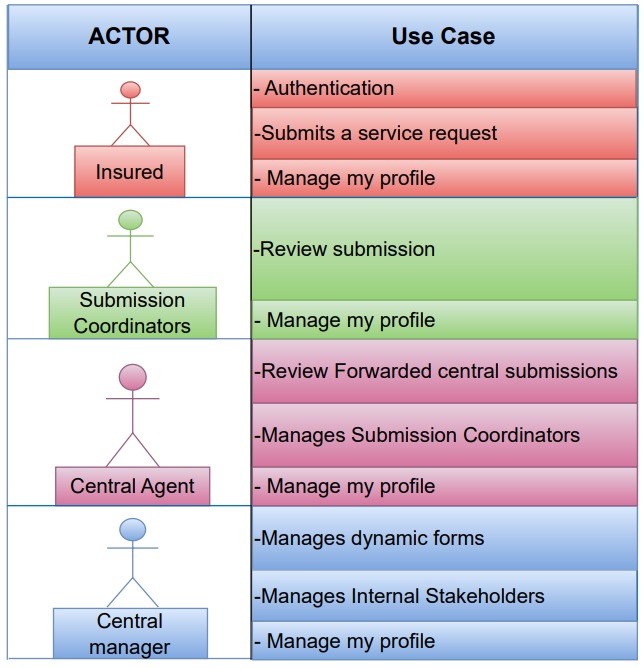
\includegraphics[width=1\textwidth]{figures/use case par acteur.png}
    \caption{Use Case Diagram by Actor.}
\end{figure}
\clearpage
\subsection{Diagramme de cas d’utilisation du premier sprint}
Le diagramme de cas d’utilisation initiale de premier sprint est présenté dans la figure suivante :
\begin{figure}[h]
    \centering
    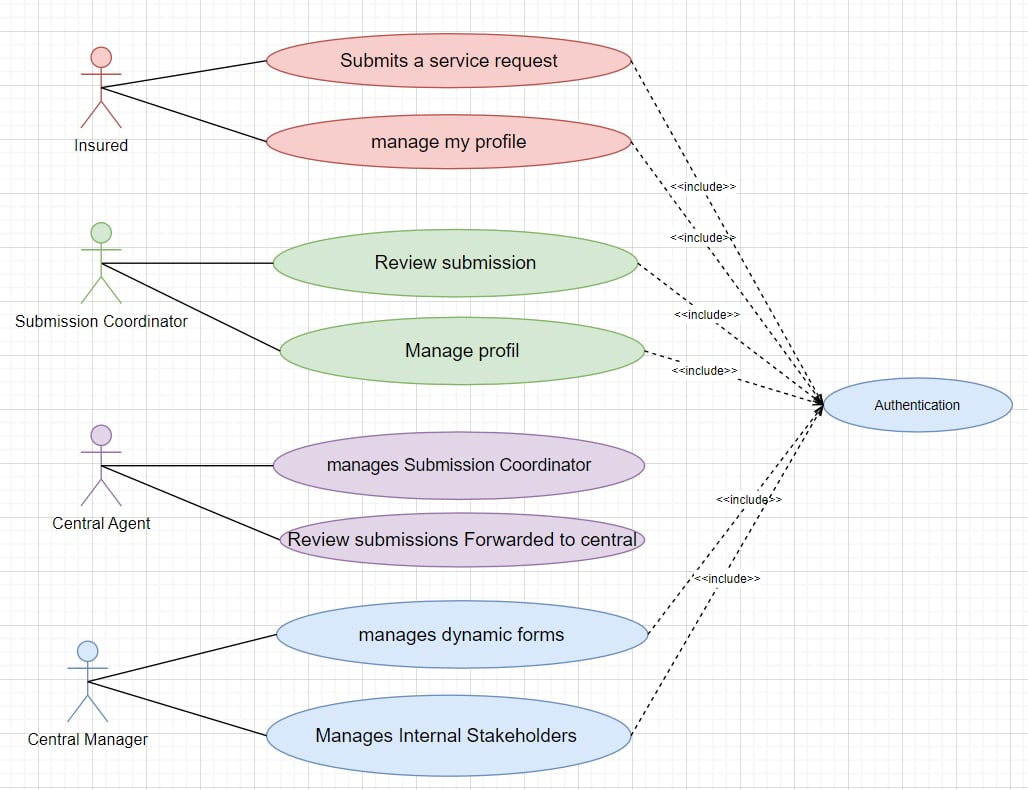
\includegraphics[width=1\textwidth]{figures/sprint1 use case.jpg}
    \caption{Use Case Diagram by Actor.}
\end{figure}
\clearpage
\subsection{Interface Prototyping}
This section aims to illustrate some prototypes of the interfaces developed during this sprint, showcasing the necessary features and interactions with our platform.
\begin{itemize}
    \item Authentication Interface Prototype
    \begin{figure}[h]
    \centering
    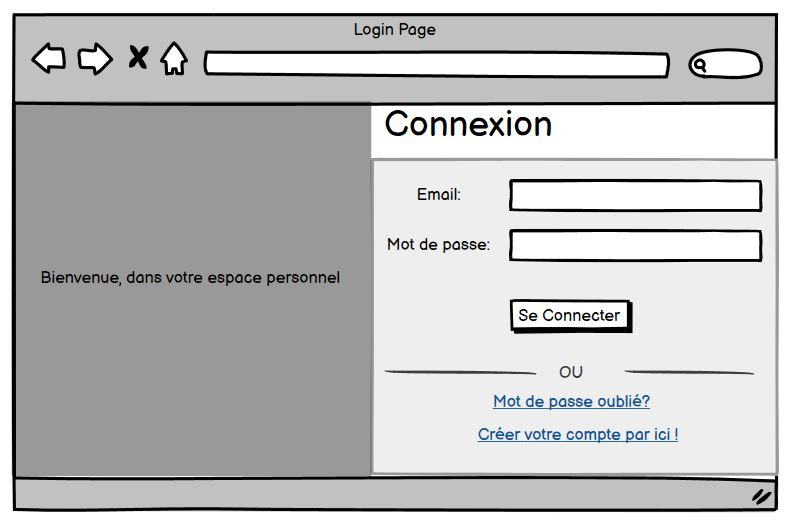
\includegraphics[width=0.9\textwidth]{figures/login.JPG}  % Replace with your image file
    \caption{Prototype of Login Page.}
\end{figure}\
\begin{figure}[h]
    \centering
    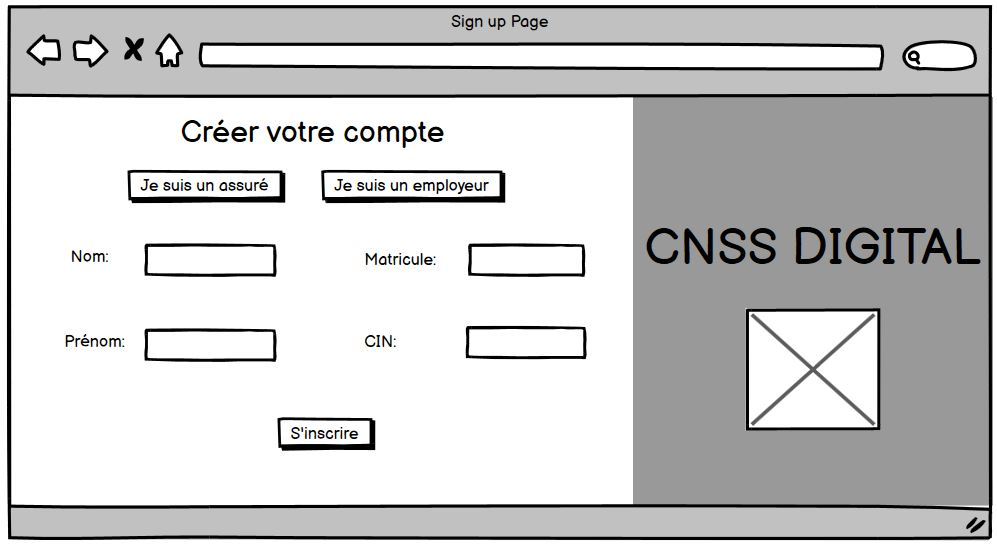
\includegraphics[width=0.9\textwidth]{figures/signup.JPG}  % Replace with your image file
    \caption{Prototype of Sign-up Page.}
\end{figure}\
\end{itemize}
\clearpage
\begin{itemize}
    \item Submission of a service request prototype
\begin{figure}[h!]
    \centering
    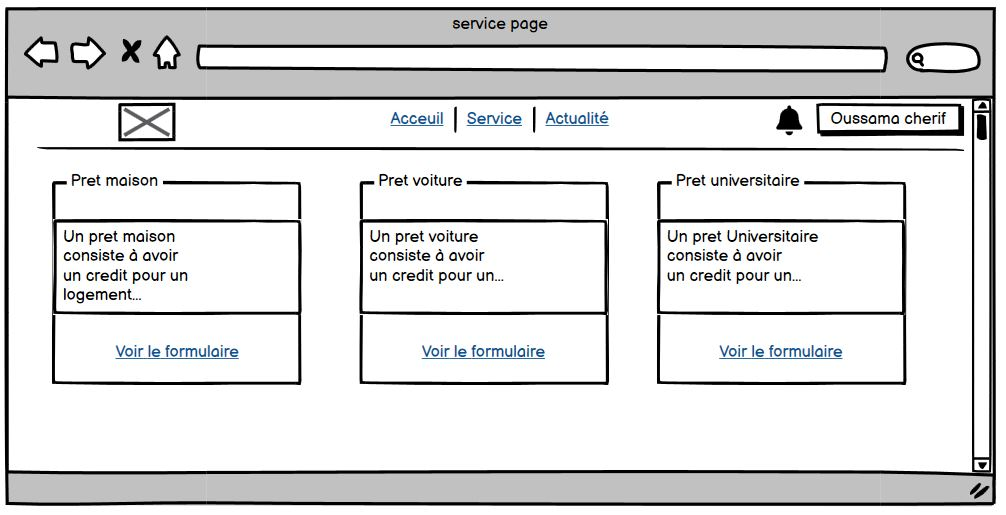
\includegraphics[width=1\textwidth]{figures/service page.JPG} 
    \caption{Prototype of Service Page.}
\end{figure}\

\begin{figure}[h]
    \centering
    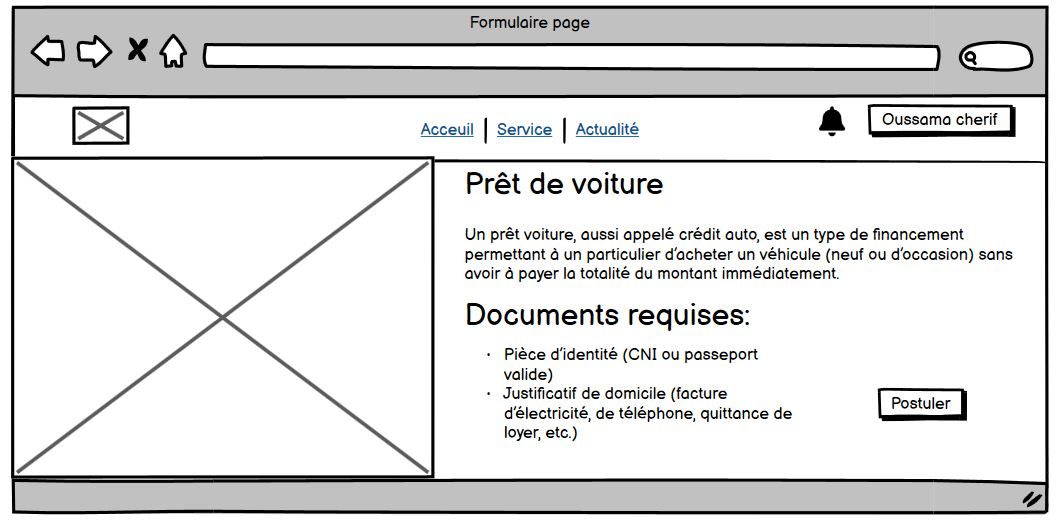
\includegraphics[width=1\textwidth]{figures/formulaire page.JPG}
    \caption{Prototype of form Page.}
\end{figure}\

\begin{figure}[h]
    \centering
    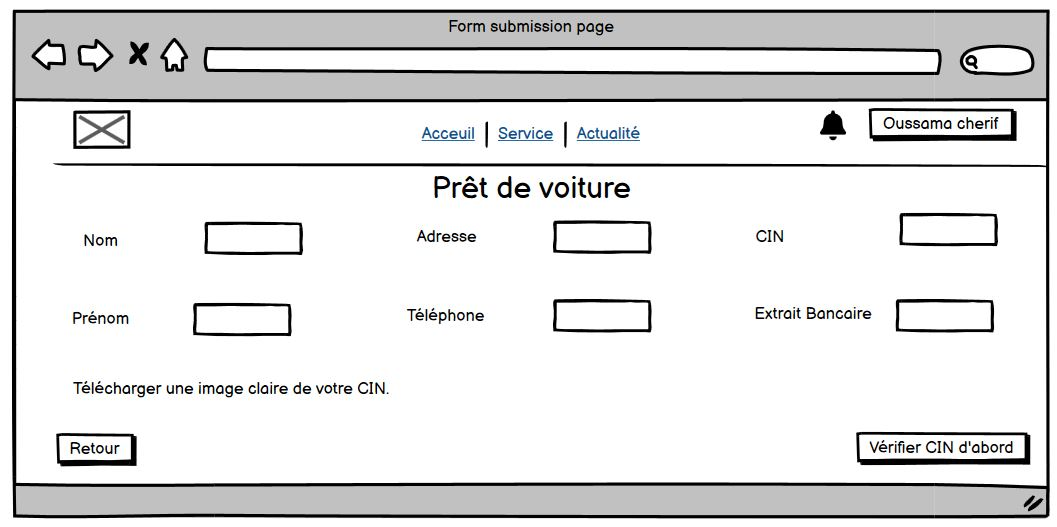
\includegraphics[width=1\textwidth]{figures/form sub page.JPG} 
    \caption{Prototype of form submission Page.}
\end{figure}\
\end{itemize}
\FloatBarrier
\begin{itemize}
    \item Managing the profile prototype
    \begin{figure}[h]
    \centering
    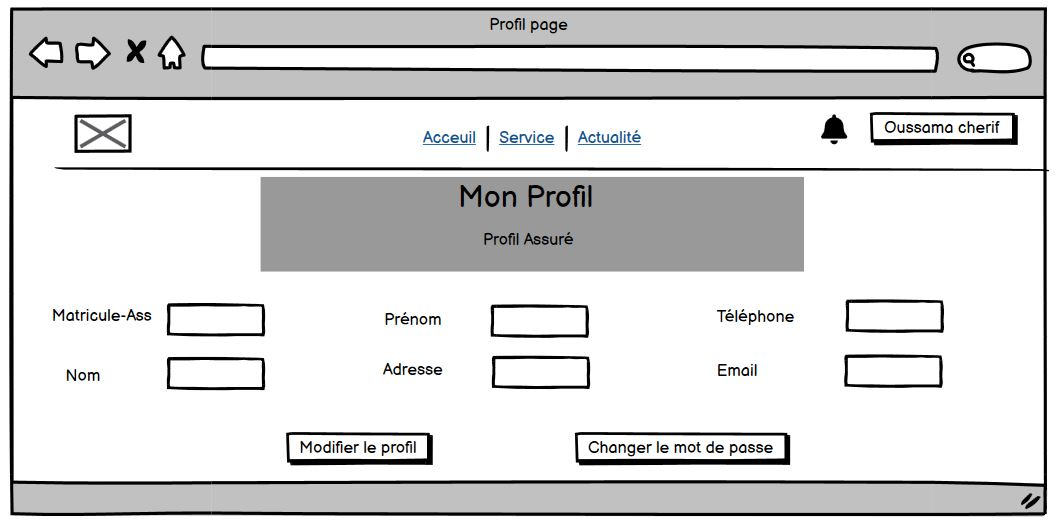
\includegraphics[width=1\textwidth]{figures/profil page.JPG} 
    \caption{Prototype of Profile Page.}
\end{figure}\
\end{itemize}
\clearpage
\begin{itemize}
    \item Review submission prototype 
    \begin{figure}[h]
    \centering
    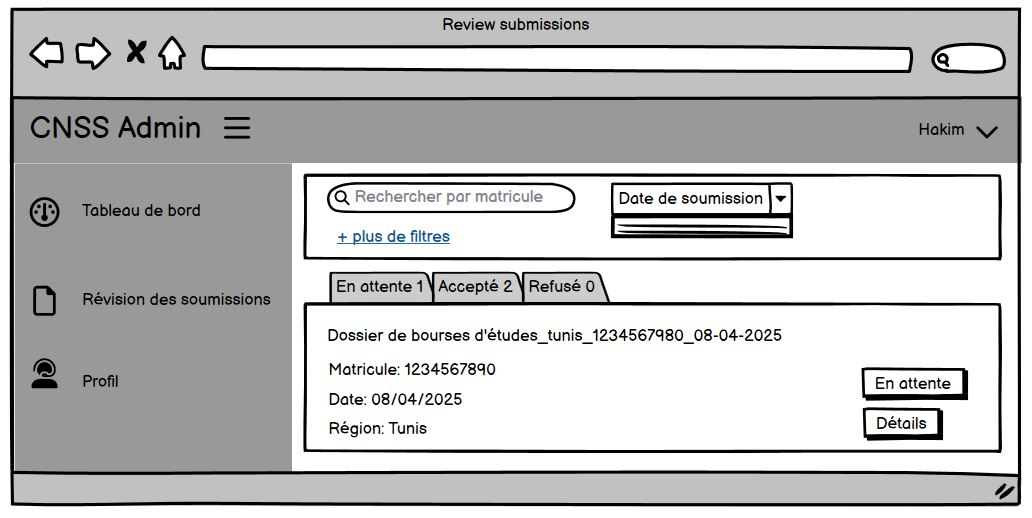
\includegraphics[width=1\textwidth]{figures/review sub.JPG}
    \caption{Prototype of Submission Review Page.}
\end{figure}\
\end{itemize}
\begin{itemize}
    \item Managing internal skateholders prototype\begin{figure}[h!]
    \centering
    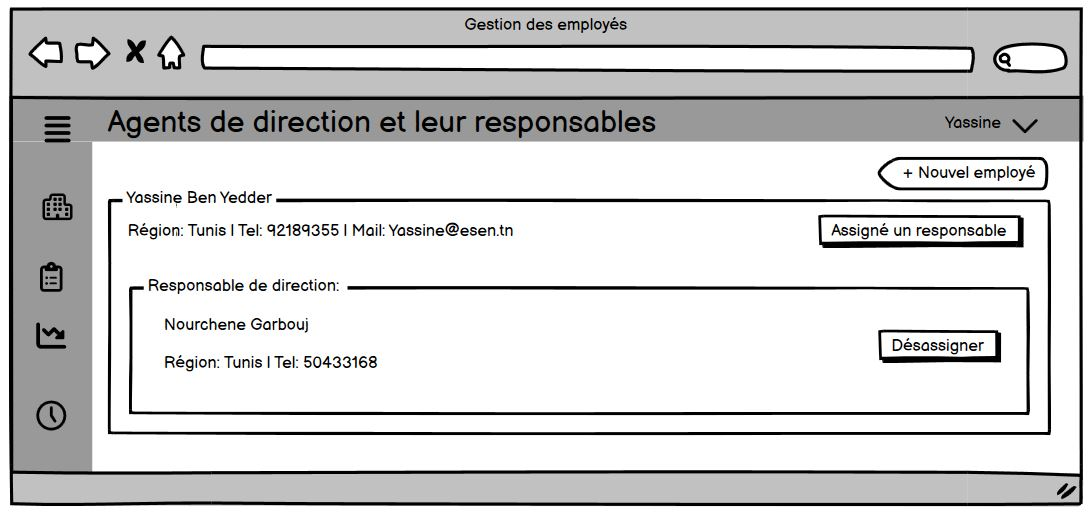
\includegraphics[width=1\textwidth]{figures/ges emp.JPG}
    \caption{Prototype of managing skateholders.}
\end{figure}\
\end{itemize}
\clearpage
\begin{itemize}
    \item managing the submission coordinators\begin{figure}[h!]
    \centering
    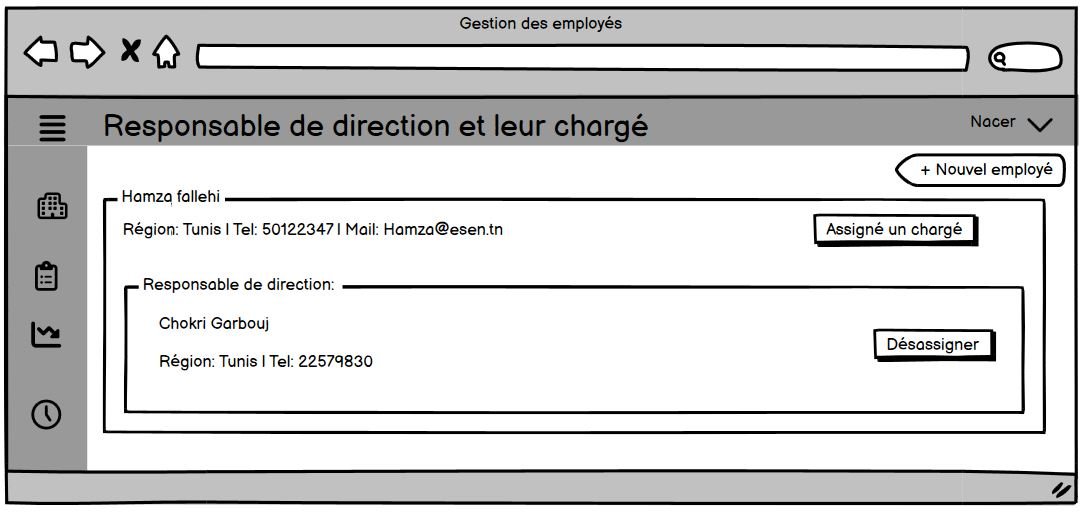
\includegraphics[width=1\textwidth]{figures/ges emp2.JPG}
    \caption{Prototype of managing the submission coordinators.}
\end{figure}\
\end{itemize}

\begin{itemize}
    \item Managing dynamic forms\begin
    {figure}[h]
    \centering
    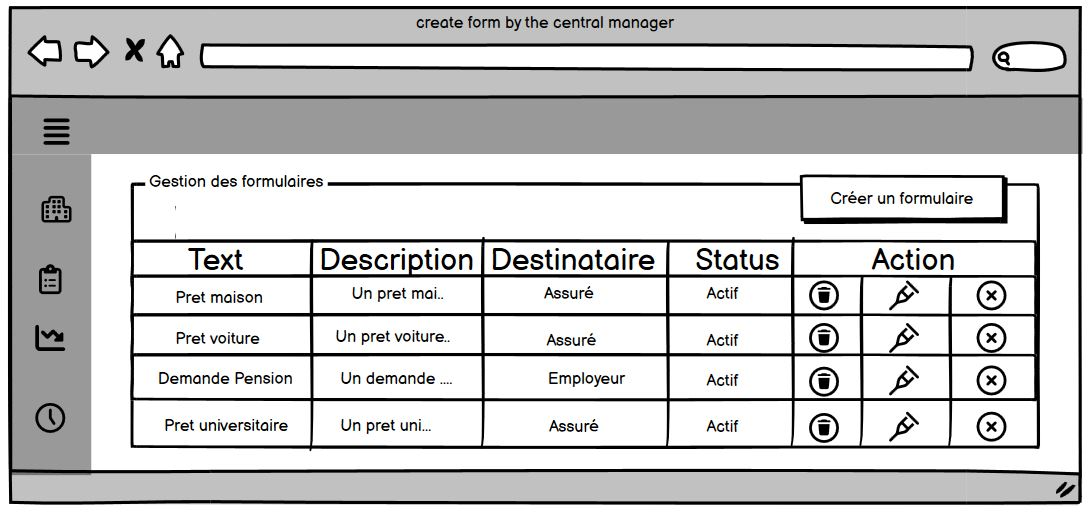
\includegraphics[width=1\textwidth]{figures/create form by the central manager.JPG}
    \caption{Prototype of the creation of a form Page.}
\end{figure}\
\end{itemize}


\clearpage

\section{Use Case Analysis}
For each use case, we will provide a textual description to explain the scenario of each and the exceptions that may occur.
\subsection{Use Case Analysis: "Authenticate"}
\subsubsection{Textual Description of the "Authenticate" Use Case}

\begin{table}[h!]
\centering
\renewcommand{\arraystretch}{1.5}
\begin{tabular}{|c|p{9cm}|}
\hline
\textbf{Use Case} & \textbf{Authenticate} \\ \hline
\textbf{Actor} & Every user of the system. \\ \hline
\textbf{Pre-condition} & The user has login credentials. \\ \hline
\textbf{Post-condition} & The user is authenticated. \\ \hline
\textbf{Main Scenario Description} & 
\begin{tabular}[c]{@{}l@{}} 
1. The system displays the login form. \\
2. The user enters their credentials (email or \\username and password) into the appropriate fields. \\
3. The user submits the form by clicking "Login." \\
4. The system verifies the information entered by the\\ user. \\
5. The system displays the appropriate interface.
\end{tabular} \\ \hline
\textbf{Alternative Scenarios} & 
\begin{tabular}[c]{@{}l@{}} 
4.a. The user enters incomplete data. \\
4.a.1: The system displays an error message. \\
4.a.2: The user repeats step 1 of the main scenario. \\
4.b. The user enters invalid data. \\
4.b.1: The system displays an error message. \\
4.b.2: The user repeats step 1 of the main scenario.
\end{tabular} \\ \hline
\end{tabular}
\caption{Use Case: Authenticate}
\end{table}
\clearpage

\begin{figure}[h!]
    \centering
    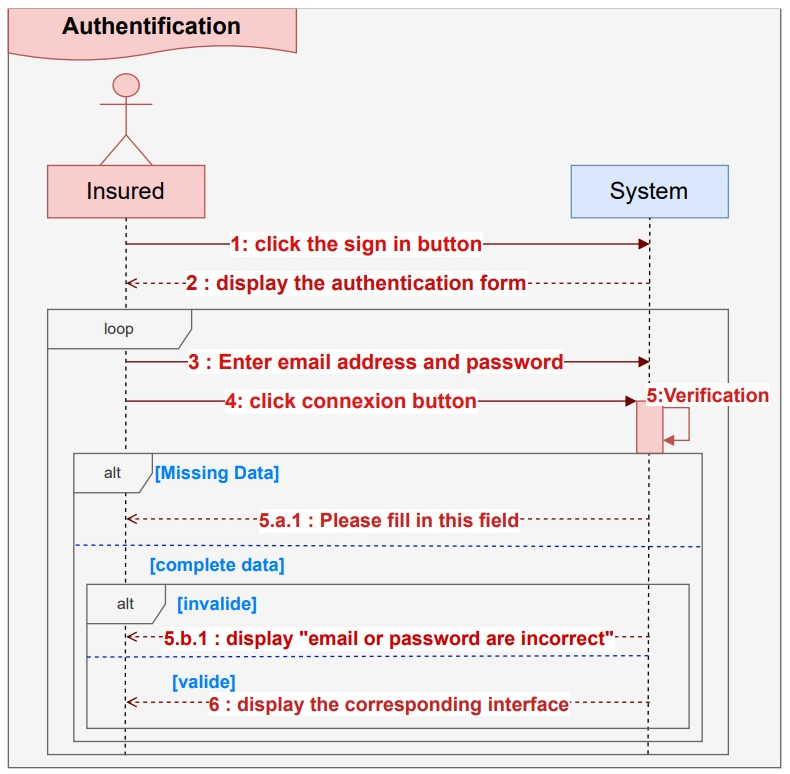
\includegraphics[width=1\textwidth]{figures/seqAuthentification.png}
    \caption{System Sequence Diagram of the "Authenticate" Use Case.}
\end{figure}
\clearpage
\subsection{Use Case Analysis: "Submit a service request"}
\subsubsection{Textual Description of the "Submit a service request" Use Case}

\begin{table}[h!]
\centering
\renewcommand{\arraystretch}{1.5}
\begin{tabular}{|c|p{9cm}|}
\hline
\textbf{Use Case} & \textbf{Submit a service request} \\ \hline
\textbf{Actor} & Insured \\ \hline
\textbf{Pre-condition} & The user is authenticated. \\ \hline
\textbf{Post-condition} & The service request is submitted and sent to the file manager.\\ 
\hline
\textbf{Main Scenario Description} & 
\begin{tabular}[c]{@{}l@{}} 
1. The insured clicks on a specific form \\
2. The system displays the form \\
3. The insured fills in the form \\
4. The insured validates the form by clicking\\ the submit button \\
5. The system verifies the entered information \\
6. The system displays a message indicating that \\the form was submitted successfully \\
\end{tabular} \\ \hline
\textbf{Alternative Scenarios} & 
\begin{tabular}[c]{@{}l@{}} 
4.a. The insured cancels the submission \\
4.a.1: The system cancels the submission. \\
4.a.2: The user repeats step 1 of the main scenario. \\
5.a One of the required fields is empty\\
5.a.1 The system displays an error message.\\
5.a.2 The process returns to step 3 of the main \\scenario.\\
5.b One of the required fields is invalid\\
5.b.1 The system displays an error message.\\
5.b.2 The process returns to step 3 of the main\\ scenario.\\
\end{tabular} \\ \hline
\end{tabular}
\caption{Use Case: Submit a service request}
\end{table}
\clearpage

\begin{figure}[h!]
    \centering
    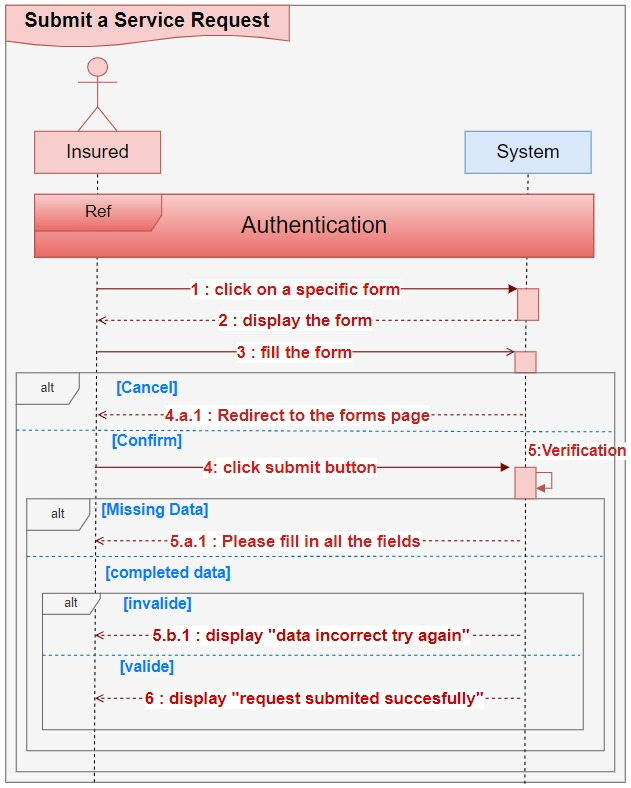
\includegraphics[width=1\textwidth]{figures/seqSubmits_service_request.png}
    \caption{System Sequence Diagram of the "Submit a service request" Use Case.}
\end{figure}\
\clearpage


\subsection{Use Case Analysis: "Manage Profile"}
\subsubsection{Refinement of the use case 'Manage Profile'}
\begin{figure}[h!]
    \centering
    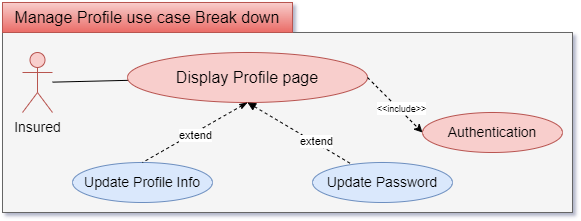
\includegraphics[width=1\textwidth]{figures/bd_manage_profile.png}
    \caption{Refinement of the use case 'Manage Profile'}
\end{figure}\


\subsubsection{Textual Description of the "Display profile page" Use Case}

\begin{table}[h!]
\centering
\renewcommand{\arraystretch}{1.5}
\begin{tabular}{|c|p{9cm}|}
\hline
\textbf{Use Case} & \textbf{Display profile page} \\ \hline
\textbf{Actor} & Every user of the system. \\ \hline
\textbf{Pre-condition} & The user is authenticated. \\ \hline
\textbf{Post-condition} & the profile page is displayed.\\ 
\hline
\textbf{Main Scenario Description} & 
\begin{tabular}[c]{@{}l@{}} 
1. The user clicks on the "My Profile" element \\
2. The system displays the profile page \\
\end{tabular} \\ \hline
\textbf{Alternative Scenarios} & 
\begin{tabular}[c]{@{}l@{}} 
None \\
\end{tabular} \\ \hline
\end{tabular}
\caption{Use Case: Display Profile page}
\end{table}
\clearpage

\begin{figure}[h!]
    \centering
    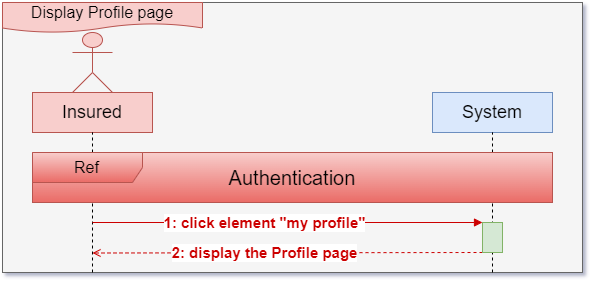
\includegraphics[width=1\textwidth]{figures/seqDisplay_profile.png}
    \caption{System Sequence Diagram of the "Display Profile page" Use Case.}
\end{figure}
\clearpage


\subsubsection{Textual Description of the "Update Profile" Use Case}

\begin{table}[h!]
\centering
\renewcommand{\arraystretch}{1.5}
\begin{tabular}{|c|p{8cm}|}
\hline
\textbf{Use Case} & \textbf{Update Profile} \\ \hline
\textbf{Actor} & Insured \\ \hline
\textbf{Pre-condition} & The insured is logged in and on their profile page. \\ \hline
\textbf{Post-condition} & The profile information is successfully updated. \\ \hline
\textbf{Main Scenario Description} & 
\begin{tabular}[c]{@{}l@{}} 
1. The insured clicks the "Update my profile" \\button. \\
2. The system displays a form to update profile\\ information. \\
3. The insured updates their profile information. \\
4. The insured clicks the "Confirm" button. \\
5. The system verifies the provided data. \\
6. The system displays a success message: \\"Profile updated\\ successfully." \\
\end{tabular} \\ \hline
\textbf{Alternative Scenarios} & 
\begin{tabular}[c]{@{}l@{}} 
4.a. The insured clicks "Cancel" instead of \\confirming. \\
4.a.1. The system redirects the insured back to \\the profile page. \\[0.2cm]
5.a. Some required fields are missing. \\
5.a.1. The system displays an error message:\\ "Please fill in this field." \\
5.a.2. The process returns to step 3 of the main \\scenario. \\
\end{tabular} \\ \hline
\end{tabular}
\caption{Use Case: Update Profile}
\end{table}
\clearpage

\begin{figure}[h!]
    \centering
    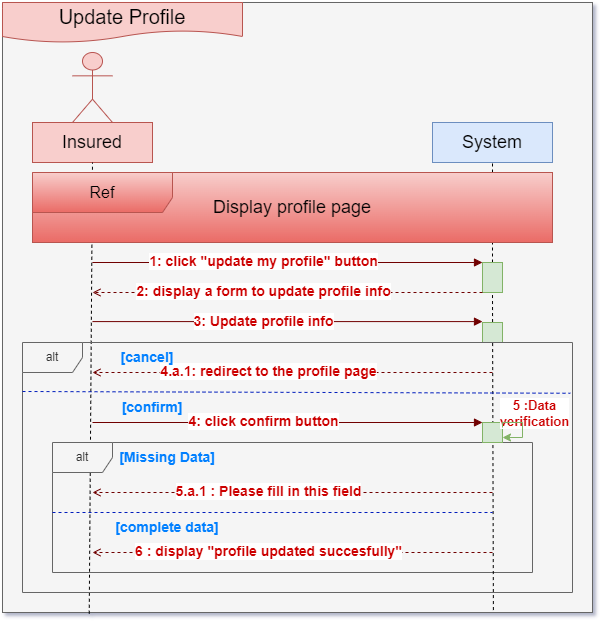
\includegraphics[width=1\textwidth]{figures/seqUpdate_profile.png}
    \caption{System Sequence Diagram of the "Update Profile" Use Case.}
\end{figure}
\clearpage


\subsubsection{Textual Description of the "Update Password" Use Case}
\begin{table}[h!]
\centering
\renewcommand{\arraystretch}{1.5}
\begin{tabular}{|c|p{9cm}|}
\hline
\textbf{Use Case} & \textbf{Update Password} \\ \hline
\textbf{Actor} & Insured \\ \hline
\textbf{Pre-condition} & The insured is logged in and on their profile page. \\ \hline
\textbf{Post-condition} & The password is successfully updated. \\ \hline
\textbf{Main Scenario Description} & 
\begin{tabular}[c]{@{}l@{}} 
1. The insured clicks the "Update my password" \\button. \\
2. The system displays a form to update the password. \\
3. The insured fills in the form. \\
4. The insured clicks the "Confirm" button. \\
5. The system verifies the provided data. \\
6. The system displays a success message: "Password \\updated successfully." \\
\end{tabular} \\ \hline
\textbf{Alternative Scenarios} & 
\begin{tabular}[c]{@{}l@{}} 
4.a. The insured clicks "Cancel". \\
4.a.1. The system redirects the user back to the profile\\ page. \\[0.2cm]
5.a. Some required fields are missing. \\
5.a.1. The system displays an error message: "Please \\fill in this field." \\
5.a.2. The process returns to step 3 of the main \\scenario. \\[0.2cm]
5.b. Provided data is invalid. \\ 
5.b.1. If the passwords do not match: \\
The system displays an error message: "Password \\doesn't match." \\
5.b.2. If the password is less than 8 characters: \\
The system displays: "Password must be 8 characters \\at least." \\
5.b.3. The process returns to step 3 of the main \\scenario. \\
\end{tabular} \\ \hline
\end{tabular}
\caption{Use Case: Update Password}
\end{table}
\clearpage

\begin{figure}[h!]
    \centering
    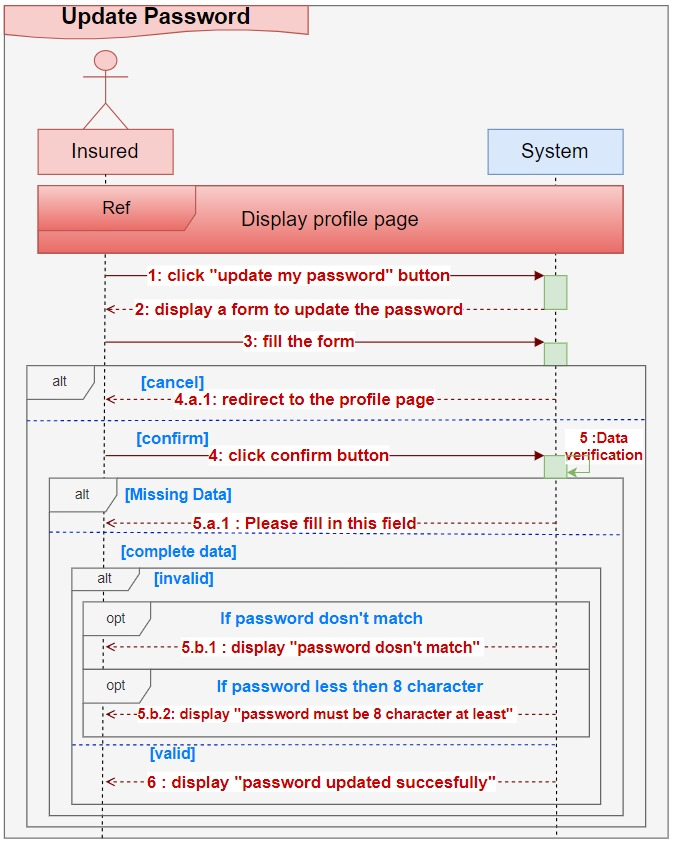
\includegraphics[width=1\textwidth]{figures/sequpdate_password.png}
    \caption{System Sequence Diagram of the "Update Password" Use Case.}
\end{figure}
\clearpage

\subsection{Use Case Analysis: "Review a Submission"}
\subsubsection{Refinement of the use case 'Review a submission'}
\begin{figure}[h!]
    \centering
    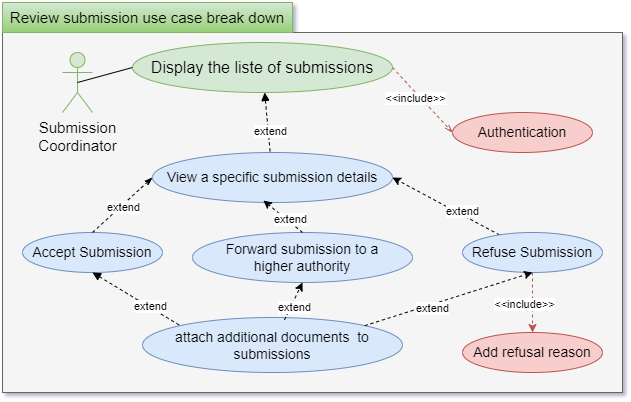
\includegraphics[width=1\textwidth]{figures/bdreview_submission.drawio.png}
    \caption{Refinement of the use case 'Review a submission'}
\end{figure}\


\subsubsection{Textual Description of the "Display submission details" Use Case}

\begin{table}[h!]
\centering
\renewcommand{\arraystretch}{1.5}
\begin{tabular}{|c|p{9cm}|}
\hline
\textbf{Use Case} & \textbf{Display submission details} \\ \hline
\textbf{Actor} & Submission Coordinators \\ \hline
\textbf{Pre-condition} & The user is authenticated. \\ \hline
\textbf{Post-condition} & the submission details is displayed.\\ 
\hline
\textbf{Main Scenario Description} & 
\begin{tabular}[c]{@{}l@{}} 
1. The user clicks on "Details" button of a specific \\submission \\
2. The system displays the submission details \\
\end{tabular} \\ \hline
\textbf{Alternative Scenarios} & 
\begin{tabular}[c]{@{}l@{}} 
None \\
\end{tabular} \\ \hline
\end{tabular}
\caption{Use Case: Display submission details}
\end{table}
\clearpage

\begin{figure}[h!]
    \centering
    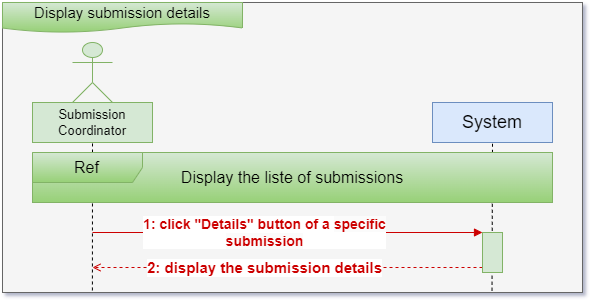
\includegraphics[width=1\textwidth]{figures/seqdisplay_submission_details.png}
    \caption{system Sequence Diagram of the "Display submission details" Use Case.'}
\end{figure}
\clearpage


\subsubsection{Textual Description of the "Refuse submission" Use Case}

\begin{table}[h!]
\centering
\renewcommand{\arraystretch}{1.5}
\begin{tabular}{|c|p{8cm}|}
\hline
\textbf{Use Case} & Refuse Submission \\ \hline
\textbf{Actor} & Submission Coordinator \\ \hline
\textbf{Pre-condition} & The coordinator is logged in and viewing the submission details. \\ \hline
\textbf{Post-condition} & The submission is marked as refused, and a reason (and optionally, documents) is saved. \\ \hline
\textbf{Main Scenario Description} & 
\begin{tabular}[c]{@{}l@{}} 
1. The coordinator clicks the "Refuse" button. \\
2. The system displays a textbox for the refusal \\reason. \\
3. The coordinator enters the refusal reason. \\
4. The coordinator clicks the "Confirm" button. \\
5. The system displays the message: \\"Submission reviewed successfully." \\
\end{tabular} \\ \hline
\textbf{Alternative Scenarios} & 
\begin{tabular}[c]{@{}l@{}} 
3.a. The coordinator wants to attach additional \\documents. \\
3.a.1. The coordinator attaches the documents. \\[0.2cm]
4.a. The coordinator clicks "Cancel". \\
4.a.1. The system redirects to the submission\\ list. \\
\end{tabular} \\ \hline
\end{tabular}
\caption{Use Case: Refuse Submission}
\end{table}

\clearpage
\begin{figure}[h!]
    \centering
    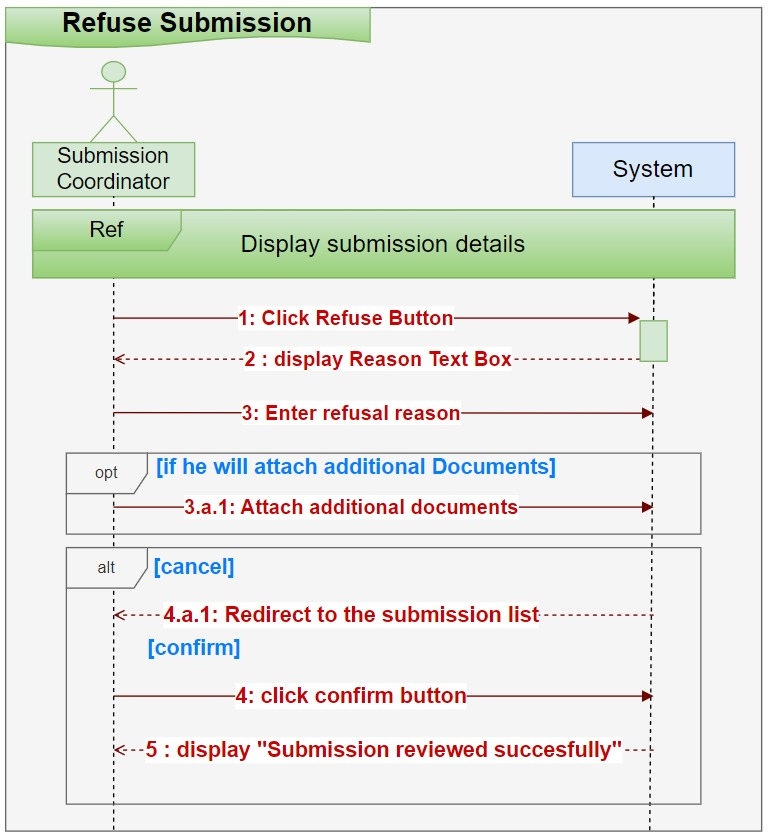
\includegraphics[width=1\textwidth]{figures/seqrefuse_submission.png}
    \caption{system Sequence Diagram of the "Refuse Submission" Use Case.'}
\end{figure}
\clearpage


\subsubsection{Textual Description of the "Escalate submission to a higher authority" Use Case}

\begin{table}[h!]
\centering
\renewcommand{\arraystretch}{1.5}
\begin{tabular}{|c|p{8cm}|}
\hline
\textbf{Use Case} & Escalate Submission to a Higher Authority \\ \hline
\textbf{Actor} & Submission Coordinator \\ \hline
\textbf{Pre-condition} & The coordinator is logged in and viewing the submission details. \\ \hline
\textbf{Post-condition} & The submission is Escalated to a higher authority successfully. \\ \hline
\textbf{Main Scenario Description} & 
\begin{tabular}[c]{@{}l@{}} 
1. The coordinator clicks the "Escalate" button. \\
2. The coordinator clicks the "Confirm" button. \\
3. The system displays the message: \\"Submission reviewed successfully." \\
\end{tabular} \\ \hline
\textbf{Alternative Scenarios} & 
\begin{tabular}[c]{@{}l@{}} 
1.a. The coordinator wants to attach additional\\ documents. \\
1.a.1. The coordinator attaches the documents. \\[0.2cm]
2.a. The coordinator clicks "Cancel". \\
2.a.1. The system redirects to the submission \\list. \\
\end{tabular} \\ \hline
\end{tabular}
\caption{Use Case: Escalate Submission to a Higher Authority}
\end{table}

\clearpage
\begin{figure}[h!]
    \centering
    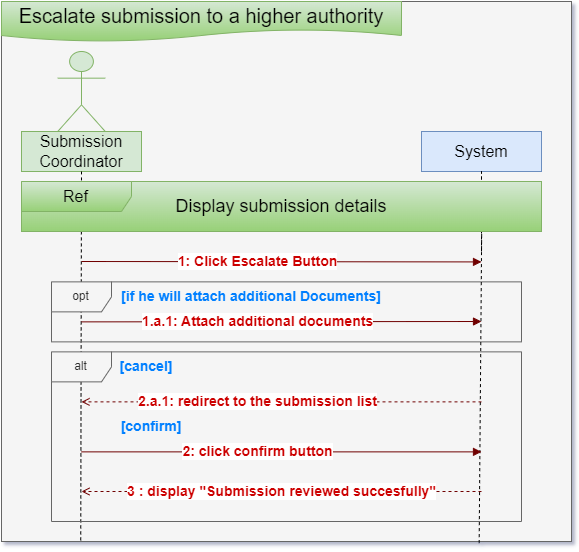
\includegraphics[width=1\textwidth]{figures/seqescalate_submission.png}
    \caption{system Sequence Diagram of the "Escalate Submission to a Higher Authority" \centering Use Case.}
\end{figure}
\clearpage
\subsection{Use Case Analysis: "Manage internal skateholders"}
\subsubsection{Refinement of the use case 'Manage internal skateholders'}
\begin{figure}[h!]
    \centering
    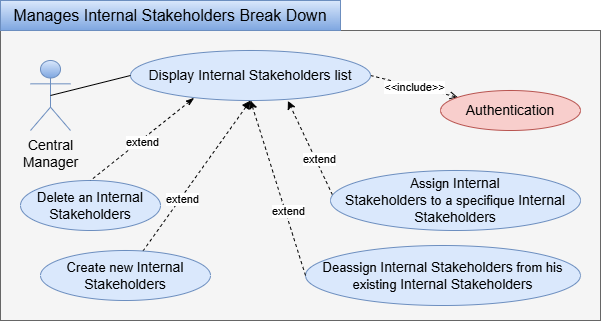
\includegraphics[width=1\textwidth]{figures/bdManages Internal Stakeholders.png}
    \caption{Refinement of the use case 'Manage Profile'}
\end{figure}\
\clearpage

\subsubsection{Textual Description of the "Create new internal stakeholders" Use Case}
\begin{table}[h!]
\centering
\renewcommand{\arraystretch}{1.5}
\begin{tabular}{|c|p{8cm}|}
\hline
\textbf{Use Case} & Create Internal Stakeholders \\ \hline
\textbf{Actor} & Central Manager \\ \hline
\textbf{Pre-condition} & The user is authenticated and on the Internal Stakeholders List page. \\ \hline
\textbf{Post-condition} & A new internal stakeholder is created and a confirmation message is displayed. \\ \hline
\textbf{Main Scenario Description} & 
\begin{tabular}[c]{@{}l@{}}
1. The user clicks on the "Create Internal \\Stakeholders" button. \\
2. The system displays a form to create a new \\internal stakeholder. \\
3. The user fills the form. \\
4. The user clicks the "Confirm" button. \\
5. The system verifies the data. \\
6. The system displays "Internal Stakeholder \\created". \\
\end{tabular} \\ \hline
\textbf{Alternative Scenarios} & 
\begin{tabular}[c]{@{}l@{}}
\textbf{4.a.} The user clicks "Cancel": \\
\quad 4.a.1. Redirect to the internal stakeholders \\list. \\
\textbf{5.a.} Data is incomplete: \\
\quad 5.a.1. System prompts: "Please fill in this \\field". \\
\end{tabular} \\ \hline
\end{tabular}
\caption{Use Case: Create Internal Stakeholders}
\end{table}
\clearpage
\begin{figure}[h!]
    \centering
    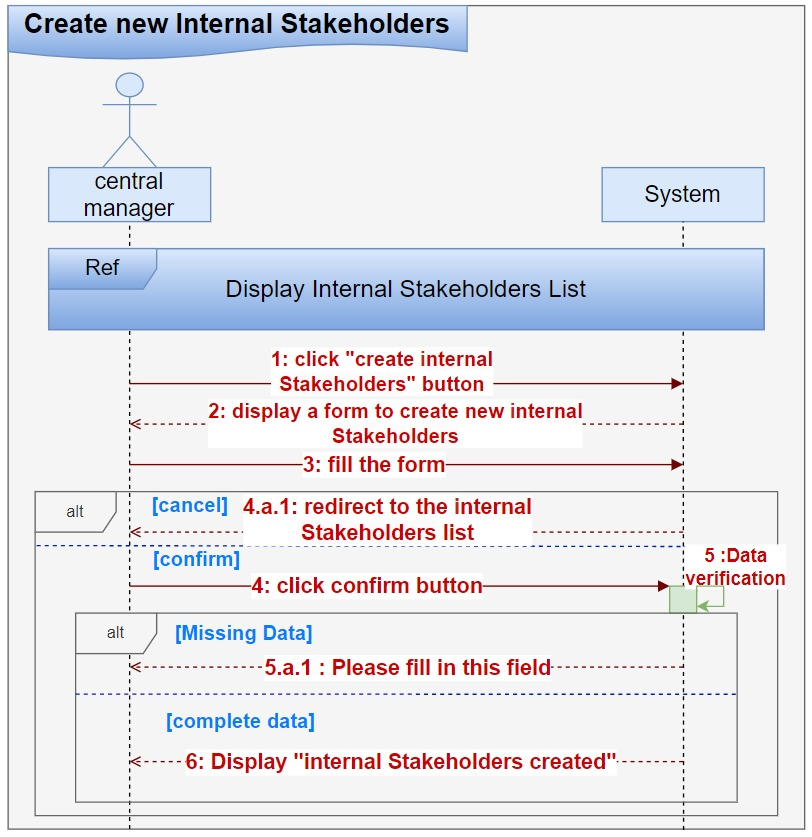
\includegraphics[width=1\textwidth]{figures/seqcreate internal skateholder.png}
    \caption{System Sequence Diagram of the "Create Internal Stakeholders" Use Case.}
\end{figure}
\clearpage


\subsubsection{Textual Description of the "Delete an internal stakeholders" Use Case}
\begin{table}[h!]
\centering
\renewcommand{\arraystretch}{1.5}
\begin{tabular}{|c|p{8cm}|}
\hline
\textbf{Use Case} & Delete an Internal Stakeholder \\ \hline
\textbf{Actor} & Central Manager \\ \hline
\textbf{Pre-condition} & The user is authenticated and viewing the Internal Stakeholders List. \\ \hline
\textbf{Post-condition} & The selected internal stakeholder is deleted, or the operation is canceled. \\ \hline
\textbf{Main Scenario Description} & 
\begin{tabular}[c]{@{}l@{}}
1. The user clicks "Delete" on an internal \\stakeholder. \\
2. The system displays a confirmation message:\\ "Are you sure you want to delete this \\employee?" \\
3. The user selects a choice (Confirm or Cancel). \\
4. If confirmed, the system displays "Employee\\ deleted successfully". \\
\end{tabular} \\ \hline
\textbf{Alternative Scenarios} & 
\begin{tabular}[c]{@{}l@{}}
\textbf{4.a.} The user clicks "Cancel": \\
\quad 4.a.1. The system redirects to the Internal \\Stakeholders List. \\
\end{tabular} \\ \hline
\end{tabular}
\caption{Use Case: Delete an Internal Stakeholder}
\end{table}
\clearpage
\begin{figure}[h!]
    \centering
    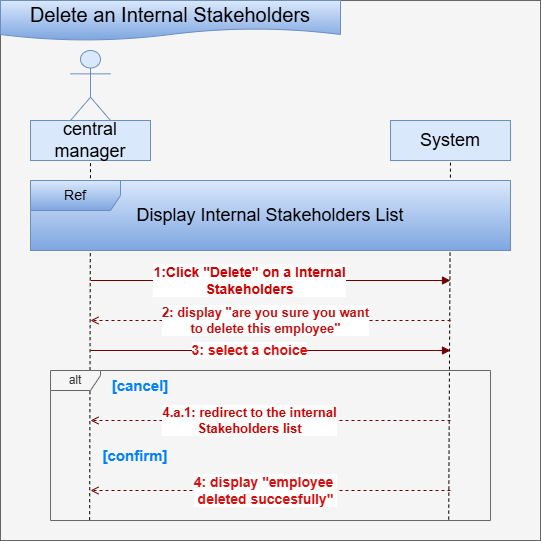
\includegraphics[width=1\textwidth]{figures/seqdelete internal.png}
    \caption{System Sequence Diagram of the "Delete an Internal Stakeholder" Use Case.}
\end{figure}
\clearpage

\subsubsection{Textual Description of the "Assign an internal stakeholder to another" Use Case}
\begin{table}[h!]
\centering
\renewcommand{\arraystretch}{1.5}
\begin{tabular}{|c|p{8cm}|}
\hline
\textbf{Use Case} & Assign an Internal Stakeholder to another \\ \hline
\textbf{Actor} & Central Manager \\ \hline
\textbf{Pre-condition} & The Central Manager is authenticated and viewing the Internal Stakeholders List. \\ \hline
\textbf{Post-condition} & The stakeholder is either successfully assigned or a validation error is shown. \\ \hline
\textbf{Main Scenario Description} & 
\begin{tabular}[c]{@{}l@{}}
1. The Central Manager selects the assignment \\type and submits. \\
2. The system performs data verification. \\
3. If the data is valid, the system displays a \\success message. \\
\end{tabular} \\ \hline
\textbf{Alternative Scenarios} & 
\begin{tabular}[c]{@{}l@{}}
\textbf{3.a.} If the assignment is invalid due to region \\conflict:
\quad 3.a.1. Display: "File manager should\\ have the same region as office supervisor." \\
\end{tabular} \\ \hline
\end{tabular}
\caption{Use Case: Assign an Internal Stakeholder to another}
\end{table}

\clearpage
\begin{figure}[h!]
    \centering
    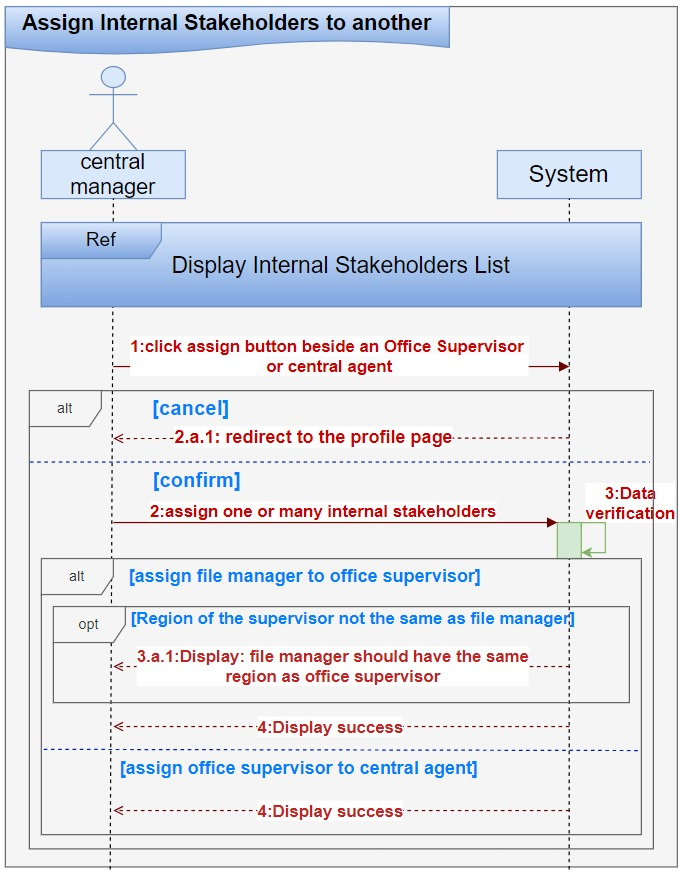
\includegraphics[width=1\textwidth]{figures/seqassign internal stakeholders.png}
    \caption{System Sequence Diagram of the "Assign an internal stakeholder to another" Use Case.}
\end{figure}
\clearpage

\subsection{Use Case Analysis: "Manage Dynamic Forms"}
\subsubsection{Refinement of the use case 'Manage dynamic forms'}
\begin{figure}[h!]
    \centering
    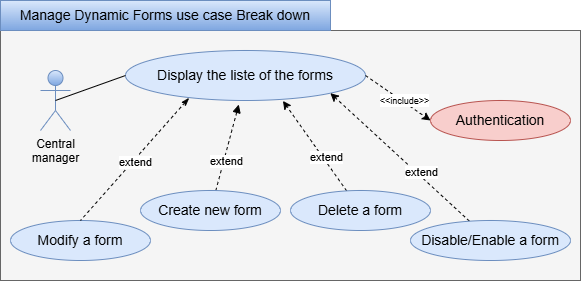
\includegraphics[width=1\textwidth]{figures/bdmanages dynamic forms-Break down.png}
    \caption{Refinement of the use case 'Manage Dynamic forms'}
\end{figure}\

\clearpage
\subsubsection{Textual Description of the "Create a new form" Use Case}
\begin{table}[h!]
\centering
\renewcommand{\arraystretch}{1.5}
\begin{tabular}{|c|p{8cm}|}
\hline
\textbf{Use Case} & Create a New Form \\ \hline
\textbf{Actor} & Central Manager \\ \hline
\textbf{Pre-condition} & The Central Manager is authenticated and on the "Forms List" page. \\ \hline
\textbf{Post-condition} & A new form is created and displayed in the list, or the operation is canceled. \\ \hline
\textbf{Main Scenario Description} & 
\begin{tabular}[c]{@{}l@{}}
1. The Central Manager clicks "Add new form". \\
2. The system displays a form to add a new \\form. \\
3. The Central Manager fills in the form. \\
4. The Central Manager clicks the "Submit" \\button. \\
5. The system verifies the submitted data. \\
6. If the data is complete, the system displays \\"Form created successfully". \\
\end{tabular} \\ \hline
\textbf{Alternative Scenarios} & 
\begin{tabular}[c]{@{}l@{}}
\textbf{4.a.} If the Central Manager clicks "Cancel": \\
\quad 4.a.1. The system redirects to the forms list. \\
\textbf{5.a.} If required data is missing: \\
\quad 5.a.1. The system displays a message:\\ "Please fill in \\this field". \\
\end{tabular} \\ \hline
\end{tabular}
\caption{Use Case: Create a New Form}
\end{table}

\clearpage
\begin{figure}[h!]
    \centering
    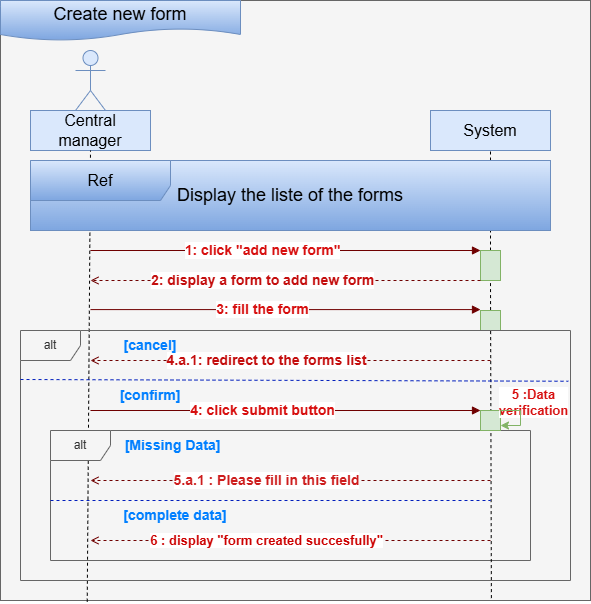
\includegraphics[width=1\textwidth]{figures/seqcreate a form..png}
    \caption{System Sequence Diagram of the "Create a new form " Use Case.}
\end{figure}
\clearpage


\subsubsection{Textual Description of the "Disable/Enable a form" Use Case}
\begin{table}[h!]
\centering
\renewcommand{\arraystretch}{1.5}
\begin{tabular}{|c|p{10cm}|}
\hline
\textbf{Use Case} & Disable/Enable a Form \\ \hline
\textbf{Actor} & Central Manager \\ \hline
\textbf{Pre-condition} & The Central Manager is authenticated and on the "Forms List" page. \\ \hline
\textbf{Post-condition} & The selected form is either disabled or enabled successfully, and the user receives a confirmation message. \\ \hline
\textbf{Main Scenario Description} & 
\begin{tabular}[c]{@{}l@{}}
1. The Central Manager clicks the "disable" button. \\
2. The system displays the message: "Form disabled \\successfully". \\
\end{tabular} \\ \hline
\textbf{Alternative Scenarios} & 
\begin{tabular}[c]{@{}l@{}}
\textbf{2.a.} If the system encounters an error: \\
\quad 2.a.1. The system displays an error message indicating\\ failure to disable the form. \\
\end{tabular} \\ \hline
\end{tabular}
\caption{Use Case: Disable/Enable a Form}
\end{table}
\begin{figure}[h!]
    \centering
    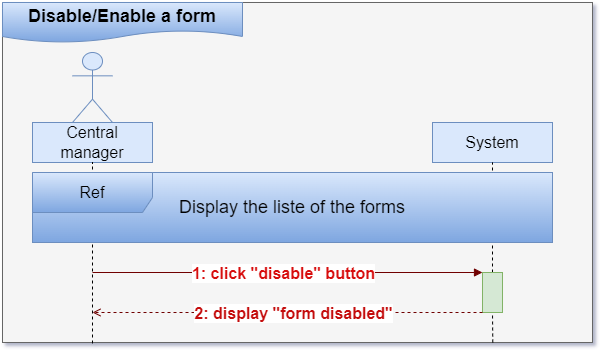
\includegraphics[width=1\textwidth]{figures/seqDisableenable a form.png}
    \caption{System Sequence Diagram of the "Disable/Enable a form " Use Case.}
\end{figure}
\clearpage

\section{Design of Use Cases}
 We proceed to the next step, where we will create the class diagrams involved for each actor, the detailed sequence diagrams of the use cases, and an object class diagram for the first sprint, following the creation of the system sequence diagrams and the textual descriptions of the use cases in the previous section.
 \subsection{The participant Class Diagram}
 \textbf{\textit{"The involvement class diagram is especially significant because it serves as a link between the use cases and software design diagrams, including interaction diagrams and the design class diagram.  Boundary, control, and entity classes are the three categories of analysis classes that are represented in the involved class diagram, along with their relationships."}}\cite{samplewebs6}
 \subsubsection{Participant class Diagram for the use case "Authenticate"}
 \begin{figure}[h!]
    \centering
    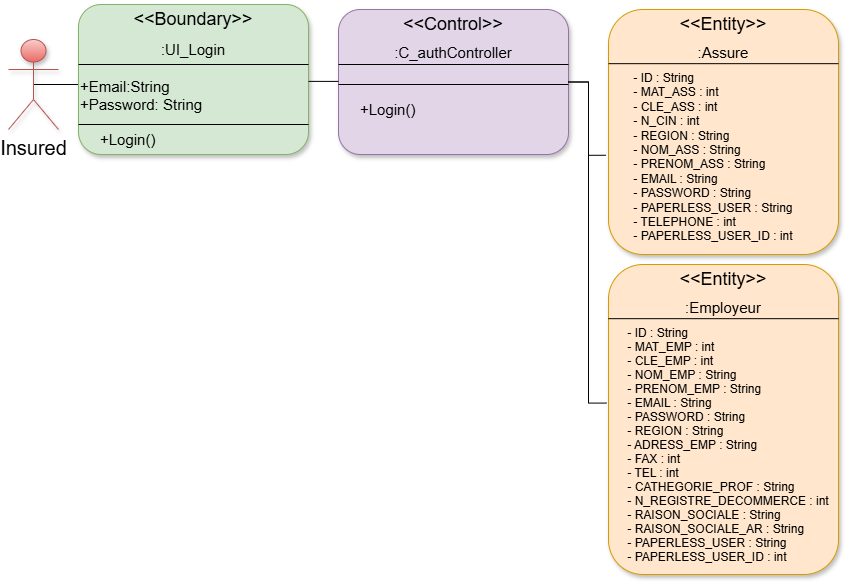
\includegraphics[width=1\textwidth]{figures/dc auth.png}
    \caption{Participant class Diagram for the use case "Authenticate"}
\end{figure}

\subsubsection{Participant class Diagram for the use case "Submit a service request"}
 \begin{figure}[h!]
    \centering
    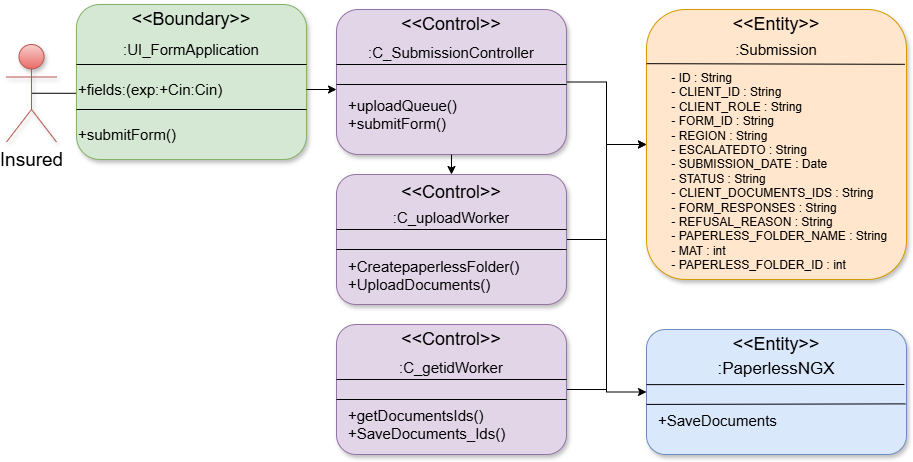
\includegraphics[width=1\textwidth]{figures/dc Submits a service request.png}
    \caption{Participant class Diagram for the use case "Submit a service request"}
\end{figure}

\subsubsection{Participant class Diagram for the use case "Manage Profile"}
 \begin{figure}[h!]
    \centering
    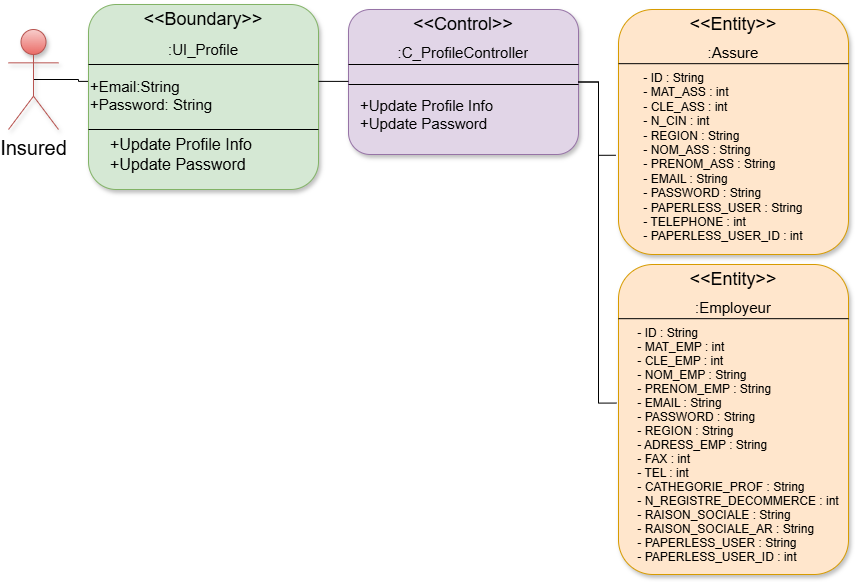
\includegraphics[width=1\textwidth]{figures/dc manage profile.png}
    \caption{Participant class Diagram for the use case "Manage Profile"}
\end{figure}
\clearpage
\subsubsection{Participant class Diagram for the use case "Review Submission"}
 \begin{figure}[h!]
    \centering
    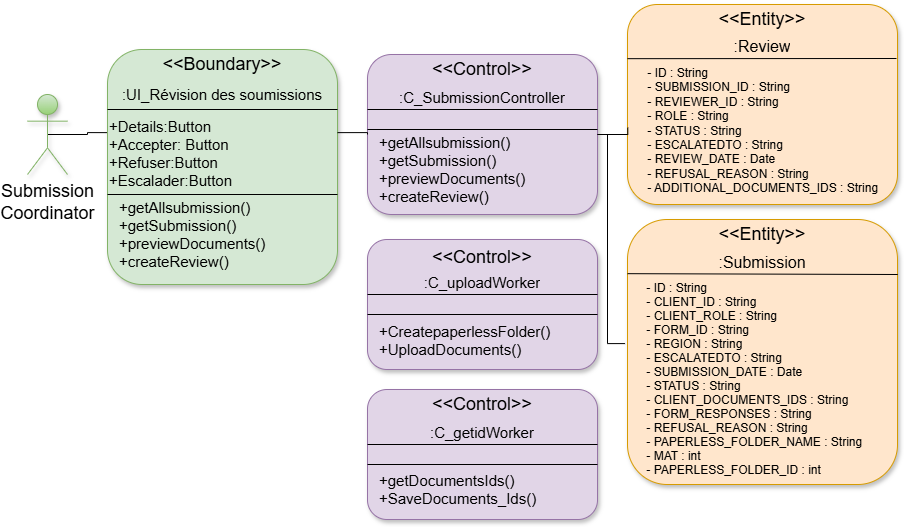
\includegraphics[width=1\textwidth]{figures/dc review submission.png}
    \caption{Participant class Diagram for the use case "Review Submission"}
\end{figure}

\subsubsection{Participant class Diagram for the use case "Manage Dynamic Forms"}
 \begin{figure}[h!]
    \centering
    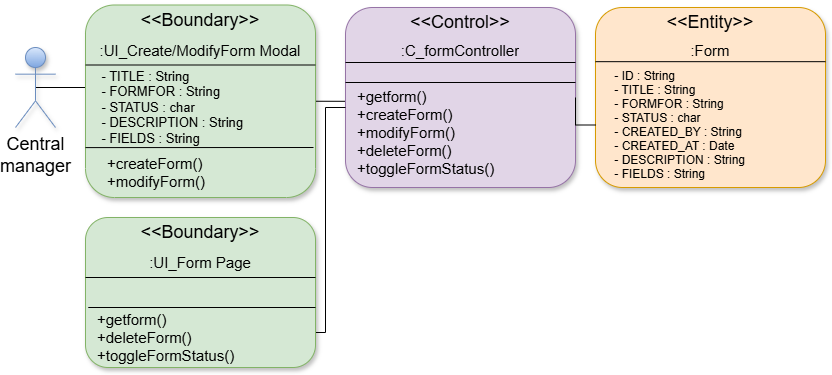
\includegraphics[width=1\textwidth]{figures/dc manageform.png}
    \caption{Participant class Diagram for the use case "Manage Dynamic Forms}
\end{figure}
\clearpage

\subsubsection{Participant class Diagram for the use case "Manage Internal Stakeholders"}
 \begin{figure}[h!]
    \centering
    \includegraphics[width=1\textwidth]{figures/dc Manages Internal Stakeholders.png}
    \caption{Participant class Diagram for the use case "Manage Internal Stakeholders}
\end{figure}

\subsection{Detailed Sequence Diagram}
\subsubsection{Detailed sequence diagram of the 'Authenticate' use case}
\clearpage
\begin{figure}[h!]
    \centering
    \includegraphics[width=1\textwidth]{figures/det authentificate.png}
    \caption{Detailed sequence diagram of the 'Authenticate' use case}
\end{figure}

\subsubsection{Detailed sequence diagram of the 'submit a service request' use case}
\begin{figure}[h!]
    \centering
    \includegraphics[width=1\textwidth]{figures/det Submits a service request.png}
    \caption{Detailed sequence diagram of the 'submit a service request' use case}
\end{figure}
\clearpage

\subsubsection{Detailed sequence diagram of the 'Manage Profile' use case}
\begin{figure}[h!]
    \centering
    \includegraphics[width=1\textwidth]{figures/det display profile.png}
    \caption{Detailed sequence diagram of the 'Display Profile' use case}
\end{figure}
\begin{figure}[h!]
    \centering
    \includegraphics[width=1\textwidth]{figures/det update profile.png}
    \caption{Detailed sequence diagram of the 'Update Profile' use case}
\end{figure}
\clearpage
\begin{figure}[h!]
    \centering
    \includegraphics[width=1\textwidth]{figures/det update password.png}
    \caption{Detailed sequence diagram of the 'Update Password' use case}
\end{figure}
\clearpage
\subsubsection{Detailed sequence diagram of the 'Review Submission' use case}
\begin{figure}[h!]
    \centering
    \includegraphics[width=1\textwidth]{figures/det review submission.png}
    \caption{Detailed sequence diagram of the 'Review Submission' use case}
\end{figure}
\clearpage
\subsubsection{Detailed sequence diagram of the 'Manage Internal stakeholders' use case}
\begin{figure}[h!]
    \centering
    \includegraphics[width=1\textwidth]{figures/det Manages Internal Stakeholders create.png}
    \caption{Detailed sequence diagram of the 'Create a new stakeholder' use case}
    \label{fig:image4}
\end{figure}
\begin{figure}[h!]
    \centering
    \includegraphics[width=1\textwidth]{figures/det Manages Internal Stakeholders delete.png}
    \caption{Detailed sequence diagram of the 'Delete a stakeholder' use case}
\end{figure}
\begin{figure}[h!]
    \centering
    \includegraphics[width=1\textwidth]{figures/det Manages Internal Stakeholders assign.png}
    \caption{Detailed sequence diagram of the 'Assign a stakeholder' use case}
\end{figure}
\clearpage
\subsubsection{Detailed sequence diagram of the 'Manage Dynamic Forms' use case}
\begin{figure}[h!]
    \centering
    \includegraphics[width=1\textwidth]{figures/det manages dynamic form create a form.png}
    \caption{Detailed sequence diagram of the 'Create a form' use case}
\end{figure}
\begin{figure}[h!]
    \centering
    \includegraphics[width=1\textwidth]{figures/det enable a form.png}
    \caption{Detailed sequence diagram of the 'Disable/Enable a form' use case}
\end{figure}
\clearpage


\section{Global class diagram of the first sprint}
\begin{figure}[h!]
    \centering
    \includegraphics[width=1\textwidth]{figures/global_class_diagram_sprint_1-diagram_de_classe_sprint_1.png}
    \caption{Global class diagram of Sprint 1.}
\end{figure}
\clearpage
\section{Implementation}
The stage of implementation, or "coding", is dedicated to implementing the user stories contained within the first sprint.
In this case, we will establish the database structure for the current sprint using the rules to map the entity-association model into the relational model.
\begin{itemize}
    \item \textbf{Rule 1:} One entity is mapped onto a table (relation).
    \item \textbf{Rule 2:} A "one-to-many" relationship results in the shifting of the primary key from the parent table to the child table as a foreign key.
    \item \textbf{Rule 3:} A "many-to-many" relationship is represented by an extra table whose primary key consists of the primary keys of related tables.
\end{itemize}

\subsection{The Database Schemas}
\begin{table}[h!]
\centering
\begin{tabular}{|l|l|l|}
\hline
\textbf{Attribut} & \textbf{Type} & \textbf{Contrainte} \\
\hline
ID & VARCHAR & PRIMARY KEY \\
NOM & VARCHAR(50) & Not Null \\
PRENOM & VARCHAR(50) & Not Null \\
REGION & VARCHAR(50) & - \\
TEL & VARCHAR(15) & - \\
EMAIL & VARCHAR(100) & UNIQUE - Not Null \\
PASSWORD & VARCHAR(255) & Not Null \\
RESPONSABLE\_ID & VARCHAR & FOREIGN KEY - Not Null \\
PAPERLESS\_USER\_ID & INT & FOREIGN KEY - Not Null \\
\hline
\end{tabular}
\caption{Table \texttt{CHARGERDEDOSSIER}}
\end{table}
\begin{table}[h!]
\centering
\begin{tabular}{|l|l|l|}
\hline
\textbf{Attribut} & \textbf{Type} & \textbf{Contrainte} \\
\hline
ID & VARCHAR & PRIMARY KEY \\
NOM & VARCHAR(50) & Not Null \\
PRENOM & VARCHAR(50) & Not Null \\
REGION & VARCHAR(50) & - \\
TEL & VARCHAR(15) & - \\
EMAIL & VARCHAR(100) & UNIQUE - Not Null \\
PASSWORD & VARCHAR(255) & Not Null \\
PAPERLESS\_USER\_ID & INT & FOREIGN KEY - Not Null \\
AGENT\_DIRECTION\_ID & VARCHAR & FOREIGN KEY \\
\hline
\end{tabular}
\caption{Table \texttt{ResponsableDirection}}
\end{table}
\begin{table}[h!]
\centering
\begin{tabular}{|l|l|l|}
\hline
\textbf{Attribut} & \textbf{Type} & \textbf{Contrainte} \\
\hline
ID & VARCHAR & PRIMARY KEY \\
NOM & VARCHAR(50) & Not Null \\
PRENOM & VARCHAR(50) & Not Null \\
REGION & VARCHAR(50) & - \\
TEL & VARCHAR(15) & - \\
EMAIL & VARCHAR(100) & UNIQUE - Not Null \\
PASSWORD & VARCHAR(255) & Not Null \\
DIRECTION\_CENTRALE\_ID & VARCHAR & FOREIGN KEY \\
PAPERLESS\_USER\_ID & INT & FOREIGN KEY - Not Null \\
\hline
\end{tabular}
\caption{Table \texttt{AgentDirection}}
\end{table}
\begin{table}[h!]
\centering
\begin{tabular}{|l|l|l|}
\hline
\textbf{Attribut} & \textbf{Type} & \textbf{Contrainte} \\
\hline
ID & VARCHAR & PRIMARY KEY \\
TEL & INT & - \\
NOM & VARCHAR(50) & Not Null \\
PRENOM & VARCHAR(50) & Not Null \\
EMAIL & VARCHAR(100) & UNIQUE - Not Null \\
PASSWORD & VARCHAR(255) & Not Null \\
PAPERLESS\_USER\_ID & INT & FOREIGN KEY - Not Null \\
\hline
\end{tabular}
\caption{Table \texttt{DirectionCentrale}}
\end{table}
\begin{table}[h!]
\centering
\begin{tabular}{|l|l|l|}
\hline
\textbf{Attribut} & \textbf{Type} & \textbf{Contrainte} \\
\hline
ID & VARCHAR & PRIMARY KEY \\
CLIENT\_ID & VARCHAR & FOREIGN KEY \\
CLIENT\_ROLE & VARCHAR(50) & Not Null \\
FORM\_ID & VARCHAR & FOREIGN KEY \\
REGION & VARCHAR(50) & - \\
ESCALATEDTO & VARCHAR & - \\
SUBMISSION\_DATE & DATE & Not Null \\
STATUS & VARCHAR(20) & Not Null \\
CLIENT\_DOCUMENTS\_IDS & VARCHAR(255) & - \\
FORM\_RESPONSES & TEXT & - \\
REFUSAL\_REASON & TEXT & - \\
PAPERLESS\_FOLDER\_NAME & VARCHAR(255) & - \\
MAT & INT & - \\
PAPERLESS\_FOLDER\_ID & INT & FOREIGN KEY - Not Null \\
\hline
\end{tabular}
\caption{Table \texttt{Submission}}
\end{table}

\begin{table}[h!]
\centering
\begin{tabular}{|l|l|l|}
\hline
\textbf{Attribut} & \textbf{Type} & \textbf{Contrainte} \\
\hline
ID & VARCHAR & PRIMARY KEY \\
TITLE & VARCHAR(255) & Not Null \\
FORM\_FOR & VARCHAR(50) & - \\
STATUS & CHAR(1) & Not Null \\
CREATED\_BY & VARCHAR(50) & - \\
CREATED\_AT & DATE & Not Null \\
DESCRIPTION & TEXT & - \\
FIELDS & TEXT & - \\
\hline
\end{tabular}
\caption{Table \texttt{Form}}
\end{table}
\begin{table}[h!]
\centering
\begin{tabular}{|l|l|l|}
\hline
\textbf{Attribut} & \textbf{Type} & \textbf{Contrainte} \\
\hline
ID & VARCHAR & PRIMARY KEY \\
SUBMISSION\_ID & VARCHAR & FOREIGN KEY \\
REVIEWER\_ID & VARCHAR & FOREIGN KEY \\
ROLE & VARCHAR(50) & - \\
STATUS & VARCHAR(50) & - \\
ESCALATEDTO & VARCHAR & - \\
REVIEW\_DATE & DATE & - \\
REFUSAL\_REASON & TEXT & - \\
ADDITIONAL\_DOCUMENTS\_IDS & TEXT & - \\
\hline
\end{tabular}
\caption{Table \texttt{Review}}
\end{table}

\begin{table}[h!]
\centering
\begin{tabular}{|l|l|l|}
\hline
\textbf{Attribut} & \textbf{Type} & \textbf{Contrainte} \\
\hline
ID & VARCHAR & PRIMARY KEY \\
MAT\_ASS & INT & UNIQUE - Not Null \\
CLE\_ASS & INT & - \\
REGION & VARCHAR(50) & - \\
NOM\_ASS & VARCHAR(50) & Not Null \\
PRENOM\_ASS & VARCHAR(50) & Not Null \\
EMAIL & VARCHAR(100) & UNIQUE - Not Null \\
PASSWORD & VARCHAR(255) & Not Null \\
PAPERLESS\_USER\_ID & INT & FOREIGN KEY - Not Null \\
TELEPHONE & INT & - \\
\hline
\end{tabular}
\caption{Table \texttt{Assure}}
\end{table}
\begin{table}[h!]
\centering
\begin{tabular}{|l|l|l|}
\hline
\textbf{Attribut} & \textbf{Type} & \textbf{Contrainte} \\
\hline
ID & VARCHAR & PRIMARY KEY \\
MAT\_EMP & INT & UNIQUE - Not Null \\
CLE\_EMP & INT & - \\
NOM\_EMP & VARCHAR(50) & Not Null \\
PRENOM\_EMP & VARCHAR(50) & Not Null \\
EMAIL & VARCHAR(100) & UNIQUE - Not Null \\
PASSWORD & VARCHAR(255) & Not Null \\
REGION & VARCHAR(50) & - \\
ADRESSE\_EMP & TEXT & - \\
FAX & INT & - \\
TEL & INT & - \\
CATEGORIE\_PROF & VARCHAR(50) & - \\
N\_REGISTRE\_DECOMMERCE & VARCHAR(50) & - \\
RAISON\_SOCIALE & VARCHAR(255) & - \\
RAISON\_SOCIALE\_AR & VARCHAR(255) & - \\
PAPERLESS\_USER\_ID & INT & FOREIGN KEY - Not Null \\
\hline
\end{tabular}
\caption{Table \texttt{Employeur}}
\end{table}
\clearpage
\subsection{The interfaces of the use cases}
\begin{figure}[h!]
    \centering
    \includegraphics[width=1\textwidth]{figures/ui-auth.png}
    \caption{Interface of the Login page.}
\end{figure}
\begin{figure}[h!]
    \centering
    \includegraphics[width=1\textwidth]{figures/ui-signup.png}
    \caption{Interface of the Sign-up page.}
\end{figure}

\begin{figure}[h!]
    \centering
    \includegraphics[width=1\textwidth]{figures/ui-servicepage.png}
    \caption{Interface of the Service page.}
\end{figure}
\begin{figure}[h!]
    \centering
    \includegraphics[width=1\textwidth]{figures/ui-detform.png}
    \caption{Interface of the Form details page.}
\end{figure}
\begin{figure}[h!]
    \centering
    \includegraphics[width=1\textwidth]{figures/ui-form.png}
    \caption{Interface of the Form page.}
\end{figure}
\begin{figure}[h!]
    \centering
    \includegraphics[width=1\textwidth]{figures/ui-reviewsub.png}
    \caption{Interface of the Review Submissions page.}
\end{figure}
\begin{figure}[h!]
    \centering
    \includegraphics[width=1\textwidth]{figures/ui-reviewsubdetails.png}
    \caption{Interface of the Review Submissions details page.}
\end{figure}
\begin{figure}[h!]
    \centering
    \includegraphics[width=1\textwidth]{figures/ui-profile.png}
    \caption{Interface of the Profile page.}
\end{figure}
\begin{figure}[h!]
    \centering
    \includegraphics[width=1\textwidth]{figures/ui-managestakeholders.png}
    \caption{Interface of the Manage Internal stakeholders page.}
\end{figure}
\begin{figure}[h!]
    \centering
    \includegraphics[width=1\textwidth]{figures/ui-manageform.png}
    \caption{Interface of Manage Form page.}
\end{figure}
\begin{figure}[h!]
    \centering
    \includegraphics[width=1\textwidth]{figures/ui-createform.png}
    \caption{Interface of create a form page.}
\end{figure}
\clearpage
\section{Tests}
\textbf{\textit{"The role of testing in the agile method is essential for the proper execution of developments. In order to ensure the reliability of the developed functionalities, it is unthinkable to pass through the sprints without having tested them beforehand: tests therefore play a crucial role."\cite{samplewebs7}}}
\subsection{Unit Tests}
We continue to work with the open source Jest unit testing framework to demonstrate in this section some examples of unit tests performed, along with the reasoning behind their implementation.
\subsection{ Unit Test for the Use Case "Submit a service request"}
\subsubsection{Reasoning} 
To test the submission of the file, we followed this reasoning:\\  
\begin{itemize}
    \item Creation of a form object.  
   \item Input of information related to the object's attributes.  
\item Insertion of the form into the database and the documents into the GED.  
\item Testing whether the form was successfully submitted.
\end{itemize}
\subsubsection{Successful Test Case "Submit a service request"} 
In the case of success, the test performed should return a positive result.
\begin{figure}[h!]
    \centering
    \includegraphics[width=1\textwidth]{figures/subScode.JPG}  % Replace with your image file
    \caption{Source code of the method submit a service request.}
\end{figure} \
\begin{figure}[h!]
    \centering
    \includegraphics[width=1\textwidth]{figures/test success submit service request.png}  
    \caption{Result of the test submitting a file request.}
\end{figure} \
\clearpage
\subsubsection{Failure Test Case "Submit a service request"}
In the case of a fail, the test performed should return a negative result.
\begin{figure}[h!]
    \centering
    \includegraphics[width=1\textwidth]{figures/subFcode.JPG}
    \caption{Source code of the method submit a service request.}
\end{figure} \
\begin{figure}[h!]
    \centering
    \includegraphics[width=1\textwidth]{figures/test fail submit service request.png}  
    \caption{Result of the test submitting a file request.}
\end{figure} \



\subsection{ Unit Test for the Use Case "Create Dynamic forms"}
\subsubsection{Reasoning} 
To test the creation of a new form, we followed this reasoning:\\  
\begin{itemize}
    \item Creation of a form object.  
   \item Input of information related to the object's attributes.  
\item Insertion of the form into the database.  
\item Testing whether the form was successfully created.
\end{itemize}
\subsubsection{Successful Test Case "Create a dynamic form"} 
In the case of success, the test performed should return a positive result.
\begin{figure}[h!]
    \centering
    \includegraphics[width=1\textwidth]{figures/createformScode.JPG}
    \caption{Source code of the method create a form.}
\end{figure} \
\clearpage
\begin{figure}[h!]
    \centering
    \includegraphics[width=1\textwidth]{figures/test succes create form.png} 
    \caption{Result of the test creating a new form.}
\end{figure} \

\subsubsection{Failure Test Case "Submit a service request"}
In the case of a fail, the test performed should return a negative result.
\begin{figure}[h!]
    \centering
    \includegraphics[width=1\textwidth]{figures/createformFcode.JPG}
    \caption{Source code of the method create a new form.}
\end{figure} \
\begin{figure}[h!]
    \centering
    \includegraphics[width=1\textwidth]{figures/test fail create form.png}  % Replace with your image file
    \caption{Result of the test creating a new form.}
\end{figure} \
\section{Sprint Review – Burndown Chart Diagram}
\textbf{\textit{"A Burndown Chart is a simple graph that shows the progress in completing tasks. In other words, it is a graphical representation of how the amount of remaining work evolves over time, within a given period."\cite{samplewebs8}}}
\begin{table}[h!]
\centering
\small
\resizebox{\textwidth}{!}{%
\begin{tabular}{|c|c|c|c|c|c|}
\hline
\textbf{DAY} & \textbf{Hours Planned} & \textbf{Hours Actual} & \textbf{Remaining Planned} & \textbf{Remaining Actual} & \textbf{Done Today} \\
\hline
0 & -  & -  & 160 & 160 & -  \\
1 & 8  & 4  & 152 & 156 &    \\
2 & 8  & 6  & 144 & 149 & 7  \\
3 & 8  & 7  & 136 & 143 & 6  \\
4 & 8  & 6  & 128 & 134 & 9  \\
5 & 8  & 7  & 120 & 133 & 1  \\
6 & 8  & 10 & 112 & 126 & 7  \\
7 & 8  & 12 & 104 & 109 & 17 \\
8 & 8  & 8  & 96  & 102 & 7  \\
9 & 8  & 6  & 88  & 90  & 12 \\
10 & 8 & 0  & 80  & 90  & 0  \\
11 & 8 & 10 & 72  & 80  & 10 \\
12 & 8 & 8  & 64  & 67  & 13 \\
13 & 8 & 8  & 56  & 60  & 7  \\
14 & 8 & 7  & 48  & 47  & 13 \\
15 & 8 & 6  & 40  & 37  & 10 \\
16 & 8 & 7  & 32  & 30  & 7  \\
17 & 8 & 6  & 24  & 25  & 5  \\
18 & 8 & 8  & 16  & 16  & 9  \\
19 & 8 & 12 & 8   & 6   & 10 \\
20 & 8 & 8  & 0   & 0   & 6  \\
\hline
\end{tabular}%
}
\caption{Burndown Chart Table for Sprint 1 (20 Days)}
\end{table}
\begin{figure}[h!]
    \centering
    \includegraphics[width=0.7\textwidth]{figures/burn down chart 1.png} 
    \caption{Burn down chart of sprint 1.}
\end{figure} \
\newpage
\begin{center}
    \doublespacing  % Increase line spacing to double spacing
    \centering
    \LARGE\textbf{Conclusion} 
    \vspace{1cm} \\
    \raggedright
\end{center}
\addcontentsline{toc}{section}{Conclusion}
In this chapter, we focused on the development of our first sprint. As a result, we now have a potentially deliverable increment of our platform.
In the next chapter, we will focus on the implementation of our second sprint.













 -









\clearpage
\chapter{Sprint 2:  Tracking, Notifications and Statistics}
\newpage
\begin{center}
    \centering
    \LARGE\textbf{Introduction} 
     \vspace{1cm} \\
   \raggedright
\end{center}
\addcontentsline{toc}{section}{Introduction}
After completing the first sprint, this chapter is dedicated to the implementation of the second sprint.  
We break down the user stories by providing a detailed description of each use case, and present the workflow of each file submission, which constitutes a major part of this sprint.  
We are going also to go through every specification of the overall design of the sprint. Therefore, we conclude with the development and testing phase.
\section{Functional Specification} 
The second sprint will address the part related to the insured tracking his own submissions and notifications, consult statics by the internal stakeholders and supervise each by his superior.

\subsection{Sprint Backlog}
The backlog dedicated to this sprint is presented in the following table:
\renewcommand{\arraystretch}{1.2}
\setlength{\tabcolsep}{6pt}

\begin{longtable}
{|>{\centering\arraybackslash}p{0.7cm}%
 |>{\raggedright\arraybackslash}p{2.5cm}%
 |>{\raggedright\arraybackslash}p{3.2cm}%
 |>{\centering\arraybackslash}p{1.2cm}%
 |>{\raggedright\arraybackslash}p{5.3cm}|}
\hline
\textbf{ID} & \textbf{User Story} & \textbf{Description} & \textbf{Task ID} & \textbf{Task} \\
\hline
\endfirsthead
\hline
1 & Track Submission Status & As an insured user, I want to track the status of my submissions to stay informed about progress. & 1.1 & Create the use case, sequence, detailed sequence, and class diagrams for “Track Submission Status”. \\
\cline{4-5}
& & & 1.2 & Implement the use case “Track Submission Status”. \\
\hline
& & & 1.3 & Test the use case “Track Submission Status”. \\
\hline
2 & View Notifications & As a user, I want to view notifications to stay updated. & 2.1 & Create the diagrams for the use case “View Notifications”. \\
\cline{4-5}
& & & 2.2 & Implement the use case “View Notifications”. \\
\cline{4-5}
& & & 2.3 & Test the use case “View Notifications”. \\
\hline
3 & View Basic Statistics & As a file manager, I want to view basic statistics to evaluate performance. & 3.1 & Create diagrams for the use case “View Basic Statistics”. \\
\cline{4-5}
& & & 3.2 & Implement the use case “View Basic Statistics”. \\
\cline{4-5}
& & & 3.3 & Test the use case “View Basic Statistics”. \\
\hline
4 & Supervise File Manager Activities & As an office supervisor, I want to supervise assigned file managers to monitor their activity. & 4.1 & Create diagrams for the use case “Supervise File Manager Activities”. \\
\hline
& & & 4.2 & Implement the use case “Supervise File Manager Activities”. \\
\cline{4-5}
& & & 4.3 & Test the use case “Supervise File Manager Activities”. \\
\hline
5 & Supervise Office Supervisor Activities & As a central agent, I want to supervise office supervisors to ensure quality of work. & 5.1 & Create diagrams for the use case “Supervise Office Supervisor Activities”. \\
\cline{4-5}
& & & 5.2 & Implement the use case “Supervise Office Supervisor Activities”. \\
\cline{4-5}
& & & 5.3 & Test the use case “Supervise Office Supervisor Activities”. \\
\hline
6 & Track Submission History & As a central agent, I want to track the history of submissions for traceability. & 6.1 & Create diagrams for the use case “Track Submission History”. \\
\cline{4-5}
& & & 6.2 & Implement the use case “Track Submission History”. \\
\cline{4-5}
& & & 6.3 & Test the use case “Track Submission History”. \\
\hline
7 & View Global Statistics & As a central manager, I want to view global statistics to analyze overall system performance. & 7.1 & Create diagrams for the use case “View Global Statistics”. \\
\cline{4-5}
& & & 7.2 & Implement the use case “View Global Statistics”. \\
\cline{4-5}
& & & 7.3 & Test the use case “View Global Statistics”. \\
\hline
\caption{Product Backlog of Sprint 2.}
\end{longtable}

\subsection{Interface Prototyping}
This section aims to illustrate some interface prototypes for this sprint, showcasing the necessary functionalities and interactions with our platform.
 \begin{figure}[h]
    \centering
    \includegraphics[width=0.9\textwidth]{figures/Tracksubstatus.JPG} 
    \caption{Prototype of Tracking the submission Page.}
\end{figure}\
 \begin{figure}[h]
    \centering
    \includegraphics[width=0.9\textwidth]{figures/notifications.JPG}  
    \caption{Prototype of The notification drop-down.}
\end{figure}\
 \begin{figure}[h]
    \centering
    \includegraphics[width=0.9\textwidth]{figures/consult basic statics.JPG} 
    \caption{Prototype of consulting the basic statics Page.}
\end{figure}\
 \begin{figure}[h]
    \centering
    \includegraphics[width=0.9\textwidth]{figures/supervise assigned file managers.JPG} 
    \caption{Prototype of the supervision of the file managers Page.}
\end{figure}\
 \begin{figure}[h]
    \centering
    \includegraphics[width=0.9\textwidth]{figures/track sub workflow.JPG} 
    \caption{Prototype of Tracking the submission history Page.}
\end{figure}\
 \begin{figure}[h!]
    \centering
    \includegraphics[width=0.9\textwidth]{figures/consult global statics.JPG}  % Replace with your image file
    \caption{Prototype of consulting the global statics Page.}
\end{figure}\

\section{Use Case Diagram of the Second Sprint}
This table provides a general classification of functionalities by actor.
 \begin{figure}[h]
    \centering
    \includegraphics[width=0.6\textwidth]{figures/use case par acteur2.png}
    \caption{Classification of the use cases per actor.}
\end{figure}\
\begin{figure}[h!]
    \centering
    \includegraphics[width=0.9\textwidth]{figures/diagram use case s2.png}
    \caption{Use Case Diagram of the Second Sprint}
\end{figure}\
\newpage
\section{Use Case Analysis}
For each use case, we will provide a textual description in order to explain the scenario for each one and the exceptions that may arise.
\subsection{Use Case Analysis "Track submission status"}
\subsubsection{Textual Description of the "Track submission status" Use Case}
\begin{table}[h]
\centering
\begin{tabular}{|l|p{8cm}|}
\hline
\textbf{Use Case} & Track Submission Status \\ \hline
\textbf{Actor} & Insured \\ \hline
\textbf{Pre-condition} & The insured user is authenticated and sees the Dashboard option. \\ \hline
\textbf{Post-condition} & The system displays the list of submissions and their statuses. \\ \hline
\textbf{Main Scenario Description} & 
\begin{tabular}[c]{@{}l@{}}
1. The insured user clicks the "Dashboard"\\ element. \\
2. The system displays the list of submissions\\ and their statuses.
\end{tabular} \\ \hline
\textbf{Alternative Scenarios} & None specified. \\ \hline
\end{tabular}
\caption{Use Case: Track Submission Status}
\end{table}
\begin{figure}[h!]
    \centering
    \includegraphics[width=0.9\textwidth]{figures/seq track sub status.JPG}
    \caption{Sequence Diagram of the use case 'Track submission status'}
\end{figure}\

\newpage
\subsection{Use Case Analysis "Consult the notifications"}
\subsubsection{Textual Description of the "Consult the notifications" Use Case}
\begin{table}[h]
\centering
\begin{tabular}{|l|p{8cm}|}
\hline
\textbf{Use Case} & Consult the Notifications \\ \hline
\textbf{Actor} & Insured \\ \hline
\textbf{Pre-condition} & The insured user is authenticated and has access to the notification alert button. \\ \hline
\textbf{Post-condition} & The system displays the list of notifications. \\ \hline
\textbf{Main Scenario Description} & 
\begin{tabular}[c]{@{}l@{}}
1. The insured user opens the Notification Alert\\ button. \\
2. The system displays the list of notifications.
\end{tabular} \\ \hline
\textbf{Alternative Scenarios} & None specified. \\ \hline
\end{tabular}
\caption{Use Case: Consult the Notifications}
\end{table}
\begin{figure}[h!]
    \centering
    \includegraphics[width=0.9\textwidth]{figures/seq consult notifications.JPG}
    \caption{Sequence Diagram of the use case 'Consult the notifications'}
\end{figure}\

\newpage
\subsection{Use Case Analysis "Supervise Assigned File Managers"}
\subsubsection{Textual Description of the "Supervise Assigned File Managers" Use Case}
\begin{table}[h]
\centering
\begin{tabular}{|l|p{8cm}|}
\hline
\textbf{Use Case} & Supervise Assigned File Managers \\ \hline
\textbf{Actor} & Office Supervisor \\ \hline
\textbf{Pre-condition} & The supervisor is authenticated \\ \hline
\textbf{Post-condition} & The file managers team's performance is displayed. \\ \hline
\textbf{Main Scenario Description} & 
\begin{tabular}[c]{@{}l@{}}
1- The supervisor opens the supervision page.\\
2- The system displays the file managers team's \\performance.
\end{tabular} \\ \hline
\textbf{Alternative Scenarios} & None specified. \\ \hline
\end{tabular}
\caption{Use Case: Supervise Assigned File Managers}
\end{table}
\begin{figure}[h!]
    \centering
    \includegraphics[width=0.9\textwidth]{figures/seq supervise assigned file managers activities.JPG}
    \caption{Sequence Diagram of the use case 'Supervise Assigned File Managers Activities'}
\end{figure}\

\newpage
\subsection{Use Case Analysis "Track Submissions Workflows History"}
\subsubsection{Textual Description of the "Track Submissions Workflows History" Use Case}
\begin{table}[h]
\centering
\begin{tabular}{|l|p{8cm}|}
\hline
\textbf{Use Case} & Track Submissions Workflows History \\ \hline
\textbf{Actor} & Central Manager \\ \hline
\textbf{Pre-condition} & The Central Manager is authenticated \\ \hline
\textbf{Post-condition} & The submission reviews and documents are displayed. \\ \hline
\textbf{Main Scenario Description} & 
\begin{tabular}[c]{@{}l@{}}
1- The central manager opens the history page.\\
2- The system displays the old submissions list.\\
3- The central manager clicks on a specific \\submission.\\
4- The system displays the submission reviews.\\
5- The central manager clicks on the "View \\Submission Documents" button.\\
6- The system displays the submission \\documents.
\end{tabular} \\ \hline
\textbf{Alternative Scenarios} & None specified. \\ \hline
\end{tabular}
\caption{Use Case: Track Submissions Workflows History}
\end{table}

\begin{figure}[h!]
    \centering
    \includegraphics[width=1\textwidth]{figures/seq track sub workflow history.png}
    \caption{Sequence Diagram of the use case 'Track Submissions Workflows History'}
\end{figure}\

\clearpage
\subsection{Use Case Analysis "Consult Global Statistics"}
\subsubsection{Textual Description of the "Consult Global Statistics" Use Case}
\begin{table}[h]
\centering
\begin{tabular}{|l|p{8cm}|}
\hline
\textbf{Use Case} & Consult Global Statistics \\ \hline
\textbf{Actor} & Central Manager \\ \hline
\textbf{Pre-condition} & The Central Manager is authenticated \\ \hline
\textbf{Post-condition} & The performance dashboard and workload metrics are displayed. \\ \hline
\textbf{Main Scenario Description} & 
\begin{tabular}[c]{@{}l@{}}
1- The Central Manager opens the dashboard \\page.\\
2- The system displays the performance \\dashboard.\\
The Central Manager reviews the following \\statistics:\\
\quad - Review Decisions Distribution\\
\quad - Reviews by Reviewer\\
\quad - Submissions by Region\\
\quad - Status by Region\\
\quad - Submission Status\\
\quad - Form Type Distribution\\
\quad - Employee Distribution\\
\quad - Regional Employees\\
\quad - User Types\\
\quad - User Regions
\end{tabular} \\ \hline
\textbf{Alternative Scenarios} & None specified. \\ \hline
\end{tabular}
\caption{Use Case: Consult Global Statistics}
\end{table}
\begin{figure}[h!]
    \centering
    \includegraphics[width=1\textwidth]{figures/seq consult global statistics.png}
    \caption{Sequence Diagram of the use case 'Consult Global Statistics'}
\end{figure}\


\clearpage
\section{Design of Use Cases}
\subsection{The participant Class Diagram}
\subsubsection{Participant class Diagram for the use case "Track Submission Status"}
\begin{figure}[h!]
    \centering
    \includegraphics[width=1\textwidth]{figures/dc track sub status.JPG}
    \caption{Participant class Diagram for the use case "Track Submission Status"}
\end{figure}\

\subsubsection{Participant class Diagram for the use case "Consult Notifications"}
\begin{figure}[h!]
    \centering
    \includegraphics[width=1\textwidth]{figures/dc consult notifications.JPG}
    \caption{Participant class Diagram for the use case "Consult Notifications"}
\end{figure}\
\clearpage
\subsubsection{Participant class Diagram for the use case "Consult Basic Statistics"}
\begin{figure}[h!]
    \centering
    \includegraphics[width=1\textwidth]{figures/dc consult basic statistics.JPG}
    \caption{Participant class Diagram for the use case "Consult Basic Statistics"}
\end{figure}\
\subsubsection{Participant class Diagram for the use case "Supervise Assigned File Managers"}
\begin{figure}[h!]
    \centering
    \includegraphics[width=1\textwidth]{figures/dc supervise assigned file managers activities.JPG}
    \caption{Participant class Diagram for the use case "Supervise Assigned File Managers"}
\end{figure}\
\clearpage
\subsubsection{Participant class Diagram for the use case "Track Submissions Workflows History"}
\begin{figure}[h!]
    \centering
    \includegraphics[width=1\textwidth]{figures/dc Track submissions Workflows history.png}
    \caption{Participant class Diagram for the use case "Track Submissions Workflows History"}
\end{figure}
\subsubsection{Participant class Diagram for the use case "Consult Global Statistics"}
\begin{figure}[h!]
    \centering
    \includegraphics[width=1\textwidth]{figures/dc Consult global statistics.png}
    \caption{Participant class Diagram for the use case "Consult Global Statistics"}
\end{figure}
\clearpage
\subsection{Detailed Sequence Diagram}
\subsubsection{Detailed sequence diagram of the 'Track Submission Status' use case}
\begin{figure}[h!]
    \centering
    \includegraphics[width=1\textwidth]{figures/det Tracks submission status.png}
    \caption{Detailed sequence diagram of the 'Track Submission Status' use case}
\end{figure}
\subsubsection{Detailed sequence diagram of the 'Consult Notifications' use case}
\begin{figure}[h!]
    \centering
    \includegraphics[width=1\textwidth]{figures/det consult notification.png}
    \caption{Detailed sequence diagram of the 'Consult Notifications' use case}
\end{figure}
\clearpage
\subsubsection{Detailed sequence diagram of the 'Consult Basic Statistics' use case}
\begin{figure}[h!]
    \centering
    \includegraphics[width=1\textwidth]{figures/det consult basic stat.png}
    \caption{Detailed sequence diagram of the 'Consult Basic Statistics' use case}
\end{figure}
\clearpage
\subsubsection{Detailed sequence diagram of the 'Supervise Assigned File Managers Activities' use case}
\begin{figure}[h!]
    \centering
    \includegraphics[width=1\textwidth]{figures/det supervise assigned file managers activities.png}
    \caption{Detailed sequence diagram of the 'Supervise Assigned File Managers Activities' use case}
\end{figure}
\subsubsection{Detailed sequence diagram of the 'Track Submissions Workflow History' use case}
\begin{figure}[h!]
    \centering
    \includegraphics[width=1\textwidth]{figures/det track sub workflow history.png}
    \caption{Detailed sequence diagram of the 'Track Submissions Workflow History' use case}
\end{figure}
\clearpage

\subsubsection{Detailed sequence diagram of the 'Consult Global Statistics' use case}
\begin{figure}[h!]
    \centering
    \includegraphics[width=1\textwidth]{figures/det consult global statistics.png}
    \caption{Detailed sequence diagram of the 'Consult Global Statistics' use case}
\end{figure}

\section{Global class diagram of the second sprint}
\begin{figure}[h!]
    \centering
    \includegraphics[width=1\textwidth]{figures/global class dia s2.jpg}
    \caption{Global class diagram of Sprint 2.}
\end{figure}
\clearpage
\section{Implementation}
In this step, we will define the structure of the current sprint's database while applying the rules for transforming the entity/association model into the relational model.
\subsection{The Database Schemas}
\begin{table}[h!]
\centering
\begin{tabular}{|l|l|l|}
\hline
\textbf{Attribut} & \textbf{Type} & \textbf{Contrainte} \\
\hline
ID & VARCHAR & PRIMARY KEY \\
NOM & VARCHAR(50) & Not Null \\
PRENOM & VARCHAR(50) & Not Null \\
REGION & VARCHAR(50) & - \\
TEL & VARCHAR(15) & - \\
EMAIL & VARCHAR(100) & UNIQUE - Not Null \\
PASSWORD & VARCHAR(255) & Not Null \\
RESPONSABLE\_ID & VARCHAR & FOREIGN KEY - Not Null \\
PAPERLESS\_USER\_ID & INT & FOREIGN KEY - Not Null \\
\hline
\end{tabular}
\caption{Table \texttt{CHARGERDEDOSSIER}}
\end{table}
\begin{table}[h!]
\centering
\begin{tabular}{|l|l|l|}
\hline
\textbf{Attribut} & \textbf{Type} & \textbf{Contrainte} \\
\hline
ID & VARCHAR & PRIMARY KEY \\
NOM & VARCHAR(50) & Not Null \\
PRENOM & VARCHAR(50) & Not Null \\
REGION & VARCHAR(50) & - \\
TEL & VARCHAR(15) & - \\
EMAIL & VARCHAR(100) & UNIQUE - Not Null \\
PASSWORD & VARCHAR(255) & Not Null \\
PAPERLESS\_USER\_ID & INT & FOREIGN KEY - Not Null \\
AGENT\_DIRECTION\_ID & VARCHAR & FOREIGN KEY \\
\hline
\end{tabular}
\caption{Table \texttt{ResponsableDirection}}
\end{table}
\clearpage
\begin{table}[h!]
\centering
\begin{tabular}{|l|l|l|}
\hline
\textbf{Attribut} & \textbf{Type} & \textbf{Contrainte} \\
\hline
ID & VARCHAR & PRIMARY KEY \\
NOM & VARCHAR(50) & Not Null \\
PRENOM & VARCHAR(50) & Not Null \\
REGION & VARCHAR(50) & - \\
TEL & VARCHAR(15) & - \\
EMAIL & VARCHAR(100) & UNIQUE - Not Null \\
PASSWORD & VARCHAR(255) & Not Null \\
DIRECTION\_CENTRALE\_ID & VARCHAR & FOREIGN KEY \\
PAPERLESS\_USER\_ID & INT & FOREIGN KEY - Not Null \\
\hline
\end{tabular}
\caption{Table \texttt{AgentDirection}}
\end{table}
\begin{table}[h!]
\centering
\begin{tabular}{|l|l|l|}
\hline
\textbf{Attribut} & \textbf{Type} & \textbf{Contrainte} \\
\hline
ID & VARCHAR & PRIMARY KEY \\
TEL & INT & - \\
NOM & VARCHAR(50) & Not Null \\
PRENOM & VARCHAR(50) & Not Null \\
EMAIL & VARCHAR(100) & UNIQUE - Not Null \\
PASSWORD & VARCHAR(255) & Not Null \\
PAPERLESS\_USER\_ID & INT & FOREIGN KEY - Not Null \\
\hline
\end{tabular}
\caption{Table \texttt{DirectionCentrale}}
\end{table}
\begin{table}[h!]
\centering
\begin{tabular}{|l|l|l|}
\hline
\textbf{Attribut} & \textbf{Type} & \textbf{Contrainte} \\
\hline
ID & VARCHAR & PRIMARY KEY \\
CLIENT\_ID & VARCHAR & FOREIGN KEY \\
CLIENT\_ROLE & VARCHAR(50) & Not Null \\
FORM\_ID & VARCHAR & FOREIGN KEY \\
REGION & VARCHAR(50) & - \\
ESCALATEDTO & VARCHAR & - \\
SUBMISSION\_DATE & DATE & Not Null \\
STATUS & VARCHAR(20) & Not Null \\
CLIENT\_DOCUMENTS\_IDS & VARCHAR(255) & - \\
FORM\_RESPONSES & TEXT & - \\
REFUSAL\_REASON & TEXT & - \\
PAPERLESS\_FOLDER\_NAME & VARCHAR(255) & - \\
MAT & INT & - \\
PAPERLESS\_FOLDER\_ID & INT & FOREIGN KEY - Not Null \\
\hline
\end{tabular}
\caption{Table \texttt{Submission}}
\end{table}
\clearpage
\begin{table}[h]
\centering
\begin{tabular}{|l|l|l|}
\hline
\textbf{Attribute} & \textbf{Type} & \textbf{Constraint} \\ \hline
ID & VARCHAR2(36) & PRIMARY KEY \\ \hline
USER\_ID & VARCHAR2(36) & Not Null \\ \hline
USER\_TYPE & VARCHAR2(20) & Check: 'assure' or 'employeur' \\ \hline
MESSAGE & VARCHAR2(2000) & Not Null \\ \hline
STATUS & VARCHAR2(20) & Check: 'unread' or 'read' \\ \hline
CREATED\_AT & DATE & Default: SYSDATE \\ \hline
RELATED\_SUBMISSION\_ID & VARCHAR2(36) & FOREIGN KEY \\ \hline
EMAIL & VARCHAR2(20) & Default: 'undone' \\ \hline
\end{tabular}
\caption{Table "NOTIFICATION"}
\end{table}
\begin{table}[h!]
\centering
\begin{tabular}{|l|l|l|}
\hline
\textbf{Attribut} & \textbf{Type} & \textbf{Contrainte} \\
\hline
ID & VARCHAR & PRIMARY KEY \\
SUBMISSION\_ID & VARCHAR & FOREIGN KEY \\
REVIEWER\_ID & VARCHAR & FOREIGN KEY \\
ROLE & VARCHAR(50) & - \\
STATUS & VARCHAR(50) & - \\
ESCALATEDTO & VARCHAR & - \\
REVIEW\_DATE & DATE & - \\
REFUSAL\_REASON & TEXT & - \\
ADDITIONAL\_DOCUMENTS\_IDS & TEXT & - \\
\hline
\end{tabular}
\caption{Table \texttt{Review}}
\end{table}

\begin{table}[h!]
\centering
\begin{tabular}{|l|l|l|}
\hline
\textbf{Attribut} & \textbf{Type} & \textbf{Contrainte} \\
\hline
ID & VARCHAR & PRIMARY KEY \\
MAT\_ASS & INT & UNIQUE - Not Null \\
CLE\_ASS & INT & - \\
REGION & VARCHAR(50) & - \\
NOM\_ASS & VARCHAR(50) & Not Null \\
PRENOM\_ASS & VARCHAR(50) & Not Null \\
EMAIL & VARCHAR(100) & UNIQUE - Not Null \\
PASSWORD & VARCHAR(255) & Not Null \\
PAPERLESS\_USER\_ID & INT & FOREIGN KEY - Not Null \\
TELEPHONE & INT & - \\
\hline
\end{tabular}
\caption{Table \texttt{Assure}}
\end{table}
\clearpage
\begin{table}[h!]
\centering
\begin{tabular}{|l|l|l|}
\hline
\textbf{Attribut} & \textbf{Type} & \textbf{Contrainte} \\
\hline
ID & VARCHAR & PRIMARY KEY \\
MAT\_EMP & INT & UNIQUE - Not Null \\
CLE\_EMP & INT & - \\
NOM\_EMP & VARCHAR(50) & Not Null \\
PRENOM\_EMP & VARCHAR(50) & Not Null \\
EMAIL & VARCHAR(100) & UNIQUE - Not Null \\
PASSWORD & VARCHAR(255) & Not Null \\
REGION & VARCHAR(50) & - \\
ADRESSE\_EMP & TEXT & - \\
FAX & INT & - \\
TEL & INT & - \\
CATEGORIE\_PROF & VARCHAR(50) & - \\
N\_REGISTRE\_DECOMMERCE & VARCHAR(50) & - \\
RAISON\_SOCIALE & VARCHAR(255) & - \\
RAISON\_SOCIALE\_AR & VARCHAR(255) & - \\
PAPERLESS\_USER\_ID & INT & FOREIGN KEY - Not Null \\
\hline
\end{tabular}
\caption{Table \texttt{Employeur}}
\end{table}
\subsection{The interfaces of the use cases}
\begin{figure}[h!]
    \centering
    \includegraphics[width=1\textwidth]{figures/ui-track sub status.png}
    \caption{Interface of Tracking submissions status page.}
\end{figure}


\begin{figure}[h!]
    \centering
    \includegraphics[width=1\textwidth]{figures/ui-consult notif.png}
    \caption{Interface of the Notification drop-down.}
\end{figure}
\begin{figure}[h!]
    \centering
    \includegraphics[width=1\textwidth]{figures/ui-consult basic stat.png}
    \caption{Interface of the basic statistics Page.}
\end{figure}
\begin{figure}[h!]
    \centering
    \includegraphics[width=1\textwidth]{figures/ui-supervise assigned fl activities.png}
    \caption{Interface of supervising the file managers activities Page.}
\end{figure}
\begin{figure}[h!]
    \centering
    \includegraphics[width=1\textwidth]{figures/ui-track workflow history.png}
    \caption{Interface of tracking the workflow history Page.}
\end{figure}
\begin{figure}[h!]
    \centering
    \includegraphics[width=1\textwidth]{figures/ui-consult global stat.png}
    \caption{Interface of the Global statistics Page.}
\end{figure}
\clearpage
\section{Tests}
During this phase, we will compare the expected results with the actual results.
This will give us the opportunity to ensure the proper functioning of the units (methods) previously implemented.
\subsection{Unit Testing}
We continue to work with the open source Jest unit testing framework to demonstrate in this section some examples of unit tests performed, along with the reasoning behind their implementation.

\subsection{ Unit Test for the Use Case "Track submission status"}
\subsubsection{Reasoning}
To test the tracking of the submission status request, we followed the reasoning below:
\begin{itemize}
    \item Create an object of type SuiviSoumission (SubmissionTracking).
    \item Set the attributes of the object with relevant information (e.g., candidate ID, submission ID, status, date of update).
    \item Simulate or retrieve a submission status update from the database.
    \item Test whether the tracking data is correctly retrieved and reflects the expected status.
\end{itemize}
\subsubsection{Successful Test Case "Track submission status"} 
In the case of success, the test performed should return a positive result.
\begin{figure}[h!]
    \centering
    \includegraphics[width=1\textwidth]{figures/track subS code.png} 
    \caption{Source code of the method track submission status.}
\end{figure} \
\begin{figure}[h!]
    \centering
    \includegraphics[width=1\textwidth]{figures/result tracksubS.png}  
    \caption{Result of the test tracking the submission status.}
\end{figure} \
\clearpage
\subsubsection{Failure Test Case "Track submission status"}
In the case of a fail, the test performed should return a negative result.
\begin{figure}[h!]
    \centering
    \includegraphics[width=1\textwidth]{figures/track subF code.png}
    \caption{Source code of the method track submission status.}
\end{figure} \
\begin{figure}[h!]
    \centering
    \includegraphics[width=1\textwidth]{figures/result tracksubF.png}  
    \caption{Result of the test tracking the submission status.}
\end{figure} \
\clearpage

\subsection{ Unit Test for the Use Case "Consult Notifications"}
\subsubsection{Reasoning}
To test consulting notifications request, we followed the reasoning below:
\begin{itemize}
    \item Create an object of type Notification.
    \item Set the necessary attributes (e.g., user ID, message content, status: read/unread, date).
    \item Simulate fetching notifications for a specific user from the database.
    \item Test whether the correct list of notifications is retrieved and if their statuses (e.g., unread) are accurately represented.
\end{itemize}
\subsubsection{Successful Test Case "Consult notifications"} 
In the case of success, the test performed should return a positive result.
\begin{figure}[h!]
    \centering
    \includegraphics[width=1\textwidth]{figures/consult notifS code.png} 
    \caption{Source code of the method consult notifications.}
\end{figure} \
\begin{figure}[h]
    \centering
    \includegraphics[width=1\textwidth]{figures/result consult notifS.png}  
    \caption{Result of the test consulting notifications.}
\end{figure} \
\
\subsubsection{Failure Test Case "Consult notifications"}
In the case of a fail, the test performed should return a negative result.
\begin{figure}[h!]
    \centering
    \includegraphics[width=1\textwidth]{figures/consult notifF code.png}
    \caption{Source code of the method consult notifications.}
\end{figure} \
\clearpage
\begin{figure}[h!]
    \centering
    \includegraphics[width=1\textwidth]{figures/result consult notifF.png}  
    \caption{Result of the test consulting notifications}
\end{figure} \


\section{Sprint Review – Burndown Chart Diagram}
The sprint review aims to inspect the results produced during this iteration.
\begin{table}[h!]
\centering
\small
\resizebox{\textwidth}{!}{%
\begin{tabular}{|c|c|c|c|c|c|}
\hline
\textbf{DAY} & \textbf{Hours Planned} & \textbf{Hours Actual} & \textbf{Remaining Planned} & \textbf{Remaining Actual} & \textbf{Done Today} \\
\hline
0  & -  & -  & 160 & 160 & -  \\
1  & 8  & 9  & 152 & 151 & 9  \\
2  & 8  & 10 & 144 & 141 & 10 \\
3  & 8  & 12 & 136 & 129 & 12 \\
4  & 8  & 12 & 128 & 117 & 12 \\
5  & 8  & 8  & 120 & 109 & 8  \\
6  & 8  & 8  & 112 & 101 & 8  \\
7  & 8  & -  & 104 & 101 & -  \\
8  & 8  & 8  & 96  & 93  & 8  \\
9  & 8  & 6  & 88  & 87  & 6  \\
10 & 8  & 5  & 80  & 82  & 5  \\
11 & 8  & 9  & 72  & 73  & 9  \\
12 & 8  & 10 & 64  & 63  & 10 \\
13 & 8  & 10 & 56  & 53  & 10 \\
14 & 8  & 8  & 48  & 45  & 8  \\
15 & 8  & -  & 40  & 40  & -  \\
16 & 8  & 10 & 32  & 35  & 10 \\
17 & 8  & 10 & 24  & 25  & 10 \\
18 & 8  & 7  & 16  & 18  & 7  \\
19 & 8  & 10 & 8   & 10  & 8  \\
20 & 8  & 8  & 0   & 0   & 8  \\
\hline
\end{tabular}%
}
\caption{Tableau de valeurs de Burndown Chart du sprint 2}
\end{table}

\begin{figure}[h!]
    \centering
    \includegraphics[width=1\textwidth]{figures/burn down chart 2.JPG} 
    \caption{Burn down chart of sprint 2.}
\end{figure} \


\newpage
\begin{center}
    \doublespacing 
    \centering
    \LARGE\textbf{Conclusion} 
    \vspace{1cm} \\
    \raggedright
\end{center}
\addcontentsline{toc}{section}{Conclusion}
In this chapter, we focused on the development of our Second sprint. As a result, we now have a potentially deliverable increment of our platform.
In the next chapter, we will focus on the implementation of our third sprint.




\clearpage
\chapter{Sprint 3:  User Access and Service Request Foundation}
\newpage
\begin{center}
    \centering
    \LARGE\textbf{Introduction} 
     \vspace{1cm} \\
   \raggedright
\end{center}
\addcontentsline{toc}{section}{Introduction}
After completing the second sprint, this chapter will be dedicated to the overall performing of the third sprint.
We will be breaking down the user stories by providing a detailed description of each use case, as the previous chapter.
We shall also present the overall design of the sprint.
Then we finally conclude with the testing and development phases.
\section{Functional Specification}
The second sprint will address the section related to managing candidate requests and interviews.
\subsection{Sprint Backlog}
The backlog dedicated to this sprint is presented in the following table:
\renewcommand{\arraystretch}{1.2}
\setlength{\tabcolsep}{6pt}

\begin{longtable}
{|>{\centering\arraybackslash}p{0.7cm}%
 |>{\raggedright\arraybackslash}p{2.5cm}%
 |>{\raggedright\arraybackslash}p{3.2cm}%
 |>{\centering\arraybackslash}p{1.2cm}%
 |>{\raggedright\arraybackslash}p{5.3cm}|}
\hline
\textbf{ID} & \textbf{User Story} & \textbf{Description} & \textbf{Task ID} & \textbf{Task} \\
\hline
1 & Consult the news & As an insured user, I want to consult the news on the platform after authentication. & 1.1 & Create the use case diagram, system sequence diagrams, detailed sequence diagrams, and class diagrams for "Consult the news". \\
\cline{4-5}
& & & 1.2 & Implement the use case "Consult the news". \\
\cline{4-5}
& & & 1.3 & Test the use case "Consult the news". \\
\hline
2 & Receive emails about my submissions & As an insured user, I want to receive emails about my submissions to stay informed about their processing. & 2.1 & Create the use case diagram, system sequence diagrams, detailed sequence diagrams, and class diagrams for "Receive emails about my submissions". \\
\cline{4-5}
& & & 2.2 & Implement the use case "Receive emails about my submissions". \\
\cline{4-5}
& & & 2.3 & Test the use case "Receive emails about my submissions". \\
\hline
3 & Reset forgotten password & As an insured user, I want to reset my password if I forget it to regain access to the platform. & 3.1 & Create the use case diagram, system sequence diagrams, detailed sequence diagrams, and class diagrams for "Reset forgotten password". \\
\cline{4-5}
& & & 3.2 & Implement the use case "Reset forgotten password". \\
\cline{4-5}
& & & 3.3 & Test the use case "Reset forgotten password". \\
\hline
4 & Manage news on the platform & As a central manager, I want to manage the news published on the platform. & 4.1 & Create the use case diagram, system sequence diagrams, detailed sequence diagrams, and class diagrams for "Manage news on the platform". \\
\cline{4-5}
& & & 4.2 & Implement the use case "Manage news on the platform". \\
\cline{4-5}
& & & 4.3 & Test the use case "Manage news on the platform". \\
\hline
5 & Recognize national identity documents & Through the OpenAI API, recognize national identity documents to automate the verification process. & 5.1 & Create the use case diagram, system sequence diagrams, detailed sequence diagrams, and class diagrams for "Recognize national identity documents". \\
\cline{4-5}
& & & 5.2 & Implement the use case "Recognize national identity documents". \\
\cline{4-5}
& & & 5.3 & Test the use case "Recognize national identity documents". \\
\hline
\caption{Product Backlog for Sprint 3}
\end{longtable}

\subsection{Interface Prototyping}
This section aims to illustrate some interface prototypes for this sprint, showcasing the necessary functionalities and interactions with our platform.
 \begin{figure}[h]
    \centering
    \includegraphics[width=0.9\textwidth]{figures/acceuil.JPG} 
    \caption{Prototype of consulting the Home Page.}
\end{figure}\
\begin{figure}[h]
    \centering
    \includegraphics[width=0.9\textwidth]{figures/actualité.JPG} 
    \caption{Prototype of consulting the Actuality Page.}
\end{figure}\
\clearpage
\begin{figure}[h]
    \centering
    \includegraphics[width=0.9\textwidth]{figures/e-mailing system.JPG} 
    \caption{Prototype of the e-mailing system Page.}
\end{figure}\
\begin{figure}[h]
    \centering
    \includegraphics[width=0.9\textwidth]{figures/reset password.JPG} 
    \caption{Prototype of resetting the password Page.}
\end{figure}\
\clearpage
\begin{figure}[h]
    \centering
    \includegraphics[width=0.9\textwidth]{figures/reset pass 2.JPG} 
    \caption{Prototype of resetting the password Page.}
\end{figure}\
\begin{figure}[h]
    \centering
    \includegraphics[width=0.9\textwidth]{figures/manage acceuil.JPG} 
    \caption{Prototype of managing the news Page.}
\end{figure}\
\clearpage
\begin{figure}[h]
    \centering
    \includegraphics[width=0.9\textwidth]{figures/AI.JPG} 
    \caption{Prototype of recognizing national documents form.}
\end{figure}\

\section{Use Case Diagram of the Third Sprint}
This table provides a general classification of functionalities by actor.
 \begin{figure}[h]
    \centering
    \includegraphics[width=0.6\textwidth]{figures/table des cas d’utilisation du sprint 3.png}
    \caption{Classification of the use cases per actor.}
\end{figure}\
\clearpage
\begin{figure}[h!]
    \centering
    \includegraphics[width=0.9\textwidth]{figures/Diagramme des cas d’utilisation du sprint 3.png}
    \caption{Use Case Diagram of the Third Sprint}
\end{figure}\
\section{Use Case Analysis}
For each use case, we will provide a textual description in order to explain the scenario for each one and the exceptions that may arise.
\subsection{Use Case Analysis "Track submission status"}
\subsubsection{Textual Description of the "Consult News" Use Case}
\begin{table}[h]
\centering
\begin{tabular}{|l|p{8cm}|}
\hline
\textbf{Use Case} & See the news \\ \hline
\textbf{Actor} & Insured \\ \hline
\textbf{Pre-condition} & The insured user is authenticated. \\ \hline
\textbf{Post-condition} & The system displays the news list. \\ \hline
\textbf{Main Scenario Description} & 
\begin{tabular}[c]{@{}l@{}}
1. The insured opens the home page.\\
2. The system displays the news list.
\end{tabular} \\ \hline
\textbf{Alternative Scenarios} & None specified. \\ \hline
\end{tabular}
\caption{Use Case: See the news}
\end{table}
\clearpage
\begin{figure}[h]
    \centering
    \includegraphics[width=0.9\textwidth]{figures/seq see the news.png}
    \caption{Sequence Diagram of the use case 'Consult News'}
\end{figure}\
\subsection{Use Case Analysis "Receive E-mails about my submission"}
\subsubsection{Textual Description of the "Receive E-mails about my submission" Use Case}
\begin{table}[h]
\centering
\begin{tabular}{|l|p{8cm}|}
\hline
\textbf{Use Case} & Receive emails about my submissions \\ \hline
\textbf{Actor} & Insured \\ \hline
\textbf{Pre-condition} & The submission has been accepted or refused. \\ \hline
\textbf{Post-condition} & An email is sent to the insured. \\ \hline
\textbf{Main Scenario Description} & 
\begin{tabular}[c]{@{}l@{}}
1. The system triggers the sending of an email.\\
2. The system sends the email via SMTP.\\
3. The email is sent successfully.
\end{tabular} \\ \hline
\textbf{Alternative Scenarios} & None specified. \\ \hline
\end{tabular}
\caption{Use Case: Receive emails about my submissions}
\end{table}
\clearpage
\begin{figure}[h]
    \centering
    \includegraphics[width=0.9\textwidth]{figures/seq Receive emails about my submissions.png}
    \caption{Sequence Diagram of the use case 'Receive e-mails about my submissions'}
\end{figure}\
\clearpage
\subsection{Use Case Analysis: "Reset forgotten password"}
\subsubsection{Textual Description of the "Reset forgotten password" Use Case}
\begin{table}[h]
\centering
\begin{tabular}{|l|p{8cm}|}
\hline
\textbf{Use Case} & Reset forgotten password \\ \hline
\textbf{Actor} & Insured \\ \hline
\textbf{Pre-condition} & The insured has forgotten their password and has access to their registered email. \\ \hline
\textbf{Post-condition} & The insured's password is successfully updated. \\ \hline
\textbf{Main Scenario Description} & 
\begin{tabular}[c]{@{}l@{}}
1. Insured clicks "Forgot Password".\\
2. Insured enters email address.\\
3. System sends reset password link via email.\\
4. Insured clicks the link from the email.\\
5. System verifies the link.\\
6. Insured enters new password and confirms.\\
7. System displays "password updated \\successfully".
\end{tabular} \\ \hline
\textbf{Alternative Scenarios} & 
\begin{tabular}[c]{@{}l@{}}
6.a.1: Passwords do not match: System displays\\ "password doesn't match".\\
6.a.2: Password less than 8 characters: System \\displays "password must be 8 characters at \\least".\\
5.a.1: Link expired (clicked after 1 hour): \\System displays "link expired".\\
5.a.2: Password updated successfully even after\\ 1 hour: System displays "password updated \\successfully".
\end{tabular} \\ \hline
\end{tabular}
\caption{Use Case: Reset forgotten password}
\end{table}
\begin{figure}[h]
    \centering
    \includegraphics[width=1\textwidth]{figures/seq reset my forgoten password.png}
    \caption{Sequence Diagram of the use case 'Reset forgotten password'}
\end{figure}\
\clearpage

\subsection{Use Case Analysis: "Manage News on the platform"}
\subsubsection{Refinement of the use case 'Manage News on the platform'}
\begin{figure}[h]
    \centering
    \includegraphics[width=1\textwidth]{figures/seq manages News-break down.png}
    \caption{Refinement of the use case 'Manage News on the platform'}
\end{figure}\
\subsubsection{Textual Description of the "Create News" Use Case}
\begin{table}[h]
\centering
\begin{tabular}{|l|p{8cm}|}
\hline
\textbf{Use Case} & Create a news \\ \hline
\textbf{Actor} & Central Manager \\ \hline
\textbf{Pre-condition} & The central manager is logged into the system. \\ \hline
\textbf{Post-condition} & The new news is displayed in the news list. \\ \hline
\textbf{Main Scenario Description} & 
\begin{tabular}[c]{@{}l@{}}
1. The central manager clicks "create new news"\\ button.\\
2. The system displays a form to create new \\news.\\
3. The central manager fills the form.\\
4. The central manager clicks confirm button.\\
5. The system verifies the data.\\
6. The system displays "Form created" and \\shows the new news.
\end{tabular} \\ \hline
\textbf{Alternative Scenarios} & 
\begin{tabular}[c]{@{}l@{}}
4.a.1. The central manager clicks cancel, the \\system redirects to the news list page.\\
5.a.1. Missing data: The system displays \\"Please fill in this field".
\end{tabular} \\ \hline
\end{tabular}
\caption{Use Case: Create a news}
\end{table}
\begin{figure}[h]
    \centering
    \includegraphics[width=1\textwidth]{figures/seq create a news.png}
    \caption{Sequence Diagram of the use case 'Create News'}
\end{figure}\
\clearpage

\subsubsection{Textual Description of the "Update News" Use Case}
\begin{table}[h]
\centering
\begin{tabular}{|l|p{8cm}|}
\hline
\textbf{Use Case} & Update a news \\ \hline
\textbf{Actor} & Central Manager \\ \hline
\textbf{Pre-condition} & The central manager is logged into the system and the news list is displayed. \\ \hline
\textbf{Post-condition} & The selected news is updated in the news list. \\ \hline
\textbf{Main Scenario Description} & 
\begin{tabular}[c]{@{}l@{}}
1. The central manager clicks "update news"\\ button.\\
2. The system displays a form to update the\\ news.\\
3. The central manager fills the form.\\
4. The central manager clicks confirm button.\\
5. The system verifies the data.\\
6. The system displays "news updated".
\end{tabular} \\ \hline
\textbf{Alternative Scenarios} & 
\begin{tabular}[c]{@{}l@{}}
4.a.1. The central manager clicks cancel, the\\ system redirects to the news list page.\\
5.a.1. Missing data: The system displays\\ "Please fill in this field".
\end{tabular} \\ \hline
\end{tabular}
\caption{Use Case: Update a news}
\end{table}
\begin{figure}[h]
    \centering
    \includegraphics[width=1\textwidth]{figures/seq update a news.png}
    \caption{Sequence Diagram of the use case 'Update News'}
\end{figure}\
\clearpage

\subsubsection{Textual Description of the "Delete News" Use Case}
\begin{table}[h]
\centering
\begin{tabular}{|l|p{8cm}|}
\hline
\textbf{Use Case} & Delete a news \\ \hline
\textbf{Actor} & Central Manager \\ \hline
\textbf{Pre-condition} & The central manager is logged into the system and the news list is displayed. \\ \hline
\textbf{Post-condition} & The selected news is deleted from the news list. \\ \hline
\textbf{Main Scenario Description} & 
\begin{tabular}[c]{@{}l@{}}
1. The central manager clicks "Delete" on a\\ news item.\\
2. The system displays "Are you sure you want \\to delete this news?".\\
3. The central manager selects confirm.\\
4. The system displays "News deleted \\successfully".
\end{tabular} \\ \hline
\textbf{Alternative Scenarios} & 
\begin{tabular}[c]{@{}l@{}}
3.a.1. The central manager selects cancel, \\the system redirects to the news list page.
\end{tabular} \\ \hline
\end{tabular}
\caption{Use Case: Delete a news}
\end{table}
\begin{figure}[h]
    \centering
    \includegraphics[width=1\textwidth]{figures/seq delete a news.png}
    \caption{Sequence Diagram of the use case 'Delete News'}
\end{figure}\
\clearpage

\subsection{Use Case Analysis "Recognize national identity documents"}
\subsubsection{Textual Description of the "Recognize national identity documents" Use Case}
\begin{table}[h]
\centering
\begin{tabular}{|l|p{8cm}|}
\hline
\textbf{Use Case} & Validate national identity documents \\ \hline
\textbf{Actor} & System \\ \hline
\textbf{Pre-condition} & National identity documents have been uploaded to the system. \\ \hline
\textbf{Post-condition} & Documents are validated and important data is extracted. \\ \hline
\textbf{Main Scenario Description} & 
\begin{tabular}[c]{@{}l@{}}
1. The system sends uploaded documents to\\ OpenAI API.\\
2. OpenAI API processes the documents.\\
3. OpenAI API returns validation status \\(valid/invalid) and extracted data.\\
4. The system receives and processes the API \\response.
\end{tabular} \\ \hline
\textbf{Alternative Scenarios} & 
\begin{tabular}[c]{@{}l@{}}
2.a.1. If documents are unreadable, API returns\\ error status.
\end{tabular} \\ \hline
\end{tabular}
\caption{Use Case: Validate national identity documents}
\end{table}
\begin{figure}[h]
    \centering
    \includegraphics[width=0.7\textwidth]{figures/seq validate national identity documents.png}
    \caption{Sequence Diagram of the use case 'Recognize national identity documents'}
\end{figure}\
\clearpage

\section{Design of Use Cases}
\subsection{The participant Class Diagram}
\subsubsection{Participant class Diagram for the use case "Consult News"}
\begin{figure}[h!]
    \centering
    \includegraphics[width=1\textwidth]{figures/dc see the news.png}
    \caption{Participant class Diagram for the use case "Consult News"}
\end{figure}\
\subsubsection{Participant class Diagram for the use case "Receive e-mails about my submissions"}
\begin{figure}[h!]
    \centering
    \includegraphics[width=0.9\textwidth]{figures/dc Receive emails about my submissions.png}
    \caption{Participant class Diagram for the use case "Receive e-mails about my submissions"}
    \clearpage
\end{figure}\
\subsubsection{Participant class Diagram for the use case "Reset forgotten password"}
\begin{figure}[h!]
    \centering
    \includegraphics[width=1\textwidth]{figures/dc reset my forgoten password.png}
    \caption{Participant class Diagram for the use case "Reset forgotten password"}
\end{figure}\
\subsubsection{Participant class Diagram for the use case "Manage news on the platform"}
\begin{figure}[h]
    \centering
    \includegraphics[width=1\textwidth]{figures/dc manages News.png}
    \caption{Participant class Diagram for the use case "Manage news on the platform"}
\end{figure}\
\subsubsection{Participant class Diagram for the use case "Recognize national identity documents"}
\begin{figure}[h]
    \centering
    \includegraphics[width=1\textwidth]{figures/dc validate national identity documents.png}
    \caption{Participant class Diagram for the use case "Recognize national identity documents"}
\end{figure}\

\subsection{Detailed Sequence Diagram}
\subsubsection{Detailed sequence diagram of the 'Consult News' use case}
\begin{figure}[h!]
    \centering
    \includegraphics[width=1\textwidth]{figures/det see the news.png}
    \caption{Detailed sequence diagram of the 'Consult News' use case}
\end{figure}
\clearpage
\subsubsection{Detailed sequence diagram of the 'Receive e-mails about my submissions' use case}
\begin{figure}[h!]
    \centering
    \includegraphics[width=1\textwidth]{figures/det Receive emails about my submissions.png}
    \caption{Detailed sequence diagram of the 'Receive e-mails about my submissions' use case}
\end{figure}
\subsubsection{Detailed sequence diagram of the 'Reset forgotten password' use case}
\begin{figure}[h!]
    \centering
    \includegraphics[width=0.8\textwidth]{figures/det reset my forgoten password.png}
    \caption{Detailed sequence diagram of the 'Reset forgotten password' use case}
\end{figure}
\clearpage
\subsubsection{Detailed sequence diagram of the 'Manage news on the platform' use case}
\begin{figure}[h!]
    \centering
    \includegraphics[width=0.8\textwidth]{figures/det create a news.png}
    \caption{Detailed sequence diagram of the 'Create news' use case}
\end{figure}
\begin{figure}[h!]
    \centering
    \includegraphics[width=0.8\textwidth]{figures/det update a news.png}
    \caption{Detailed sequence diagram of the 'Update news' use case}
\end{figure}
\clearpage
\begin{figure}[h!]
    \centering
    \includegraphics[width=1\textwidth]{figures/det delete a news.png}
    \caption{Detailed sequence diagram of the 'Delete news' use case}
\end{figure}
\clearpage
\section{Global class diagram of the third sprint}
\begin{figure}[h!]
    \centering
    \includegraphics[width=1\textwidth]{figures/global class diagram sprint 3.png}
    \caption{Global class diagram of Sprint 3.}
\end{figure}


\section{Implementation}
In this step, we will define the structure of the current sprint's database while applying the rules for transforming the entity/association model into the relational model.
\subsection{The Database Schemas}
\begin{table}[h!]
\centering
\begin{tabular}{|l|l|l|}
\hline
\textbf{Attribut} & \textbf{Type} & \textbf{Contrainte} \\
\hline
id & VARCHAR & PRIMARY KEY \\
type & VARCHAR(50) & - \\
mat & VARCHAR(50) & - \\
cle & VARCHAR(50) & - \\
email & VARCHAR(100) & - \\
code & VARCHAR(50) & - \\
createdAt & TIMESTAMP & - \\
expiresAt & TIMESTAMP & - \\
\hline
\end{tabular}
\caption{Table \texttt{VERIFICATION\_CODES}}
\end{table}
\clearpage
\begin{table}[h!]
\centering
\begin{tabular}{|l|l|l|}
\hline
\textbf{Attribut} & \textbf{Type} & \textbf{Contrainte} \\
\hline
ID & VARCHAR & PRIMARY KEY \\
CLIENT\_ID & VARCHAR & FOREIGN KEY \\
CLIENT\_ROLE & VARCHAR(50) & - \\
FORM\_ID & VARCHAR & FOREIGN KEY \\
REGION & VARCHAR(50) & - \\
ESCALATEDTO & VARCHAR & - \\
SUBMISSION\_DATE & DATE & - \\
STATUS & VARCHAR(50) & - \\
CLIENT\_DOCUMENTS\_IDS & VARCHAR & - \\
FORM\_RESPONSES & TEXT & - \\
REFUSAL\_REASON & TEXT & - \\
PAPERLESS\_FOLDER\_NAME & VARCHAR(100) & - \\
MAT & INT & - \\
PAPERLESS\_FOLDER\_ID & INT & - \\
\hline
\end{tabular}
\caption{Table \texttt{Submission}}
\end{table}

\begin{table}[h!]
\centering
\begin{tabular}{|l|l|l|}
\hline
\textbf{Attribut} & \textbf{Type} & \textbf{Contrainte} \\
\hline
ID & VARCHAR & PRIMARY KEY \\
TEL & INT & - \\
NOM & VARCHAR(50) & Not Null \\
PRENOM & VARCHAR(50) & Not Null \\
EMAIL & VARCHAR(100) & UNIQUE - Not Null \\
PASSWORD & VARCHAR(255) & Not Null \\
PAPERLESS\_USER\_ID & INT & - \\
\hline
\end{tabular}
\caption{Table \texttt{DIRECTIONCENTRALE}}
\end{table}

\begin{table}[h!]
\centering
\begin{tabular}{|l|l|l|}
\hline
\textbf{Attribut} & \textbf{Type} & \textbf{Contrainte} \\
\hline
ID & VARCHAR & PRIMARY KEY \\
MAT\_ASS & INT & - \\
CLE\_ASS & INT & - \\
N\_CIN & INT & - \\
REGION & VARCHAR(50) & - \\
NOM\_ASS & VARCHAR(50) & Not Null \\
PRENOM\_ASS & VARCHAR(50) & Not Null \\
EMAIL & VARCHAR(100) & UNIQUE - Not Null \\
PASSWORD & VARCHAR(255) & Not Null \\
PAPERLESS\_USER & VARCHAR(100) & - \\
TELEPHONE & INT & - \\
PAPERLESS\_USER\_ID & INT & - \\
\hline
\end{tabular}
\caption{Table \texttt{Assure}}
\end{table}

\begin{table}[h!]
\centering
\begin{tabular}{|l|l|l|}
\hline
\textbf{Attribut} & \textbf{Type} & \textbf{Contrainte} \\
\hline
ID & VARCHAR & PRIMARY KEY \\
MAT\_EMP & INT & - \\
CLE\_EMP & INT & - \\
NOM\_EMP & VARCHAR(50) & Not Null \\
PRENOM\_EMP & VARCHAR(50) & Not Null \\
EMAIL & VARCHAR(100) & UNIQUE - Not Null \\
PASSWORD & VARCHAR(255) & Not Null \\
REGION & VARCHAR(50) & - \\
ADRESS\_EMP & TEXT & - \\
FAX & INT & - \\
TEL & INT & - \\
CATHEOORIE\_PROF & VARCHAR(50) & - \\
N\_REGISTRE\_DECOMMERCE & INT & - \\
RAISON\_SOCIALE & VARCHAR(100) & - \\
PAPERLESS\_USER & VARCHAR(100) & - \\
PAPERLESS\_USER\_ID & INT & - \\
\hline
\end{tabular}
\caption{Table \texttt{Employeur}}
\end{table}

\begin{table}[h!]
\centering
\begin{tabular}{|l|l|l|}
\hline
\textbf{Attribut} & \textbf{Type} & \textbf{Contrainte} \\
\hline
ID & VARCHAR & PRIMARY KEY \\
TITRE & VARCHAR(100) & Not Null \\
CONTENU & TEXT & Not Null \\
DATE\_PUBLICATION & VARCHAR(50) & - \\
ADMIN\_ID & VARCHAR & FOREIGN KEY \\
\hline
\end{tabular}
\caption{Table \texttt{NEWS}}
\end{table}
\clearpage
\begin{table}[h!]
\centering
\begin{tabular}{|l|l|l|}
\hline
\textbf{Attribut} & \textbf{Type} & \textbf{Contrainte} \\
\hline
ID & VARCHAR & PRIMARY KEY \\
TITLE & VARCHAR(100) & Not Null \\
FORMEOR & VARCHAR(50) & - \\
STATUS & CHAR(1) & - \\
CREATED\_BY & VARCHAR & FOREIGN KEY \\
CREATED\_AT & DATE & - \\
DESCRIPTION & TEXT & - \\
FIELDS & TEXT & - \\
\hline
\end{tabular}
\caption{Table \texttt{Form}}
\end{table}
\subsection{The interfaces of the use cases}
\begin{figure}[h!]
    \centering
    \includegraphics[width=1\textwidth]{figures/ui-see news1.png}
    \caption{Interface of consulting news 1.}
\end{figure}
\clearpage
\begin{figure}[h!]
    \centering
    \includegraphics[width=1\textwidth]{figures/ui-see news2.png}
    \caption{Interface of consulting news 2.}
\end{figure}
\vspace{1.5cm}
\begin{figure}[h!]
    \centering
    \includegraphics[width=1\textwidth]{figures/ui-see news3.png}
    \caption{Interface of consulting news 3.}
\end{figure}
\clearpage
\begin{figure}[h!]
    \centering
    \includegraphics[width=1\textwidth]{figures/ui-receive emails.png}
    \caption{Interface of receiving an e-mail.}
\end{figure}
\vspace{1.5cm}
\begin{figure}[h!]
    \centering
    \includegraphics[width=1\textwidth]{figures/ui-reset pass1.png}
    \caption{Interface of resetting password 1.}
\end{figure}
\clearpage
\begin{figure}[h!]
    \centering
    \includegraphics[width=1\textwidth]{figures/ui-reset pass2.png}
    \caption{Interface of resetting password 2.}
\end{figure}
\vspace{1.5cm}
\begin{figure}[h!]
    \centering
    \includegraphics[width=1\textwidth]{figures/ui-reset pass3.png}
    \caption{Interface of resetting password 3.}
\end{figure}
\clearpage
\begin{figure}[h!]
    \centering
    \includegraphics[width=1\textwidth]{figures/ui-manage news.png}
    \caption{Interface of managing the news.}
\end{figure}
\vspace{1.5cm}
\begin{figure}[h!]
    \centering
    \includegraphics[width=1\textwidth]{figures/ui-recognize ai.png}
    \caption{Interface of the form (recognize documents on file fields).}
\end{figure}
\clearpage
\section{Tests}
During this phase, we will compare the expected results with the actual results.
This will give us the opportunity to ensure the proper functioning of the units (methods) previously implemented.

\subsection{Unit Testing}
We continue to work with the open source Jest unit testing framework to demonstrate in this section some examples of unit tests performed, along with the reasoning behind their implementation.

\subsection{ Unit Test for the Use Case "Create news"}
\subsubsection{Reasoning}
To test the creation of news request, we followed the reasoning below:
\begin{itemize}
    \item Create an object of type News.
    \item Fill in the attributes of the object (e.g., title, content, publication date, author).
    \item Insert the news article into the database.
    \item Test whether the news article was successfully created and stored.
\end{itemize}
\subsubsection{Successful Test Case "Create News"} 
In the case of success, the test performed should return a positive result.
\begin{figure}[h!]
    \centering
    \includegraphics[width=1\textwidth]{figures/create newsS code.png} 
    \caption{Source code of the method create news.}
\end{figure} \
\begin{figure}[h!]
    \centering
    \includegraphics[width=1\textwidth]{figures/result create newsS.png}  
    \caption{Result of the test creating news.}
\end{figure} \
\clearpage
\subsubsection{Failure Test Case "Create News"}
In the case of a fail, the test performed should return a negative result.
\begin{figure}[h!]
    \centering
    \includegraphics[width=1\textwidth]{figures/create newsF code.png}
    \caption{Source code of the method create news.}
\end{figure} \
\begin{figure}[h!]
    \centering
    \includegraphics[width=1\textwidth]{figures/result create newsF.png}  
    \caption{Result of the test Creating news.}
\end{figure} \
\clearpage

\subsection{ Unit Test for the Use Case "Validate national identity documents"}
\subsubsection{Reasoning}
To test the validation of the national identity documents request, we followed the reasoning below:
\begin{itemize}
    \item Create an object of type PieceIdentite (IdentityDocument).
    \item Fill in the attributes of the object (e.g., document number, type, expiration date, holder's name).
    \item Apply validation rules (e.g., format checks, expiration status, duplication check).
    \item Test whether the identity document is considered valid or rejected based on the validation logic.
\end{itemize}
\subsubsection{Successful Test Case "Validate national identity documents"} 
In the case of success, the test performed should return a positive result.
\begin{figure}[h!]
    \centering
    \includegraphics[width=1\textwidth]{figures/validate idS code.png} 
    \caption{Source code of the method Validating national identity documents.}
\end{figure} \
\begin{figure}[h]
    \centering
    \includegraphics[width=1\textwidth]{figures/result validate national idS.png}  
    \caption{Result of the test Validating national identity documentss.}
\end{figure} \
\
\subsubsection{Failure Test Case "Validate national identity documents"}
In the case of a fail, the test performed should return a negative result.
\begin{figure}[h!]
    \centering
    \includegraphics[width=1\textwidth]{figures/validate idF code.png}
    \caption{Source code of the method Validating national identity documents.}
\end{figure} \
\clearpage
\begin{figure}[h!]
    \centering
    \includegraphics[width=1\textwidth]{figures/result validate national idF.png}  
    \caption{Result of the test Validating national identity documentss}
\end{figure} \

\section{Sprint Review – Burndown Chart Diagram}
The sprint review aims to inspect the results produced during this iteration.
\begin{table}[h!]
\centering
\small
\resizebox{\textwidth}{!}{%
\begin{tabular}{|c|c|c|c|c|c|}
\hline
\textbf{DAY} & \textbf{Hours Planned} & \textbf{Hours Actual} & \textbf{Remaining Planned} & \textbf{Remaining Actual} & \textbf{Done Today} \\
\hline
0  & -  & -  & 160 & 160 & -  \\
1  & 8  & 10 & 152 & 150 & 10 \\
2  & 8  & 10 & 144 & 140 & 10 \\
3  & 8  & 6  & 136 & 134 & 6  \\
4  & 8  & 6  & 128 & 128 & 6  \\
5  & 8  & 10 & 120 & 118 & 10 \\
6  & 8  & 10 & 112 & 108 & 10 \\
7  & 8  & 10 & 104 & 98  & 10 \\
8  & 8  & 10 & 96  & 88  & 10 \\
9  & 8  & 6  & 88  & 82  & 6  \\
10 & 8  & 9  & 80  & 73  & 9  \\
11 & 8  & 7  & 72  & 66  & 7  \\
12 & 8  & 6  & 64  & 60  & 6  \\
13 & 8  & 7  & 56  & 53  & 7  \\
14 & 8  & 8  & 48  & 45  & 8  \\
15 & 8  & 7  & 40  & 38  & 7  \\
16 & 8  & 8  & 32  & 30  & 8  \\
17 & 8  & 8  & 24  & 22  & 8  \\
18 & 8  & 9  & 16  & 13  & 9  \\
19 & 8  & 6  & 8   & 7   & 6  \\
20 & 8  & 9  & 0   & 0   & 9  \\
\hline
\end{tabular}%
}
\caption{Burndown Chart Table for Sprint 3 (20 Days)}
\end{table}
\clearpage
\begin{figure}[h!]
    \centering
    \includegraphics[width=1\textwidth]{figures/burn down chart 3.JPG} 
    \caption{Burn down chart of sprint 3.}
\end{figure} \

\begin{center}
    \doublespacing 
    \centering
    \LARGE\textbf{Conclusion} 
    \vspace{1cm} \\
    \raggedright
\end{center}
\addcontentsline{toc}{section}{Conclusion}
In this chapter, we focused on the development of our Third sprint. As a result, we now have a potentially deliverable increment of our platform.
In the following chapter, we will detail the resources that we used while conducting our project.




\clearpage
\chapter{Cloture Phase}
\newpage
\begin{center}
    \centering
    \LARGE\textbf{Introduction} 
     \vspace{1cm} \\
   \raggedright
\end{center}
\addcontentsline{toc}{section}{Introduction}
In this final chapter, we will explain the ultimate phase of a development cycle using Scrum.  
First, we will start by listing the hardware and software development environment that we used during the realization of our project.  
Then, we will present a deployment diagram that shows the architecture of our application, as well as a schematic representation of the various tasks carried out throughout the project.
\section{Development Environment}
To begin, we will present the hardware and software environment that we are using.
\subsection{Hardware Environment}
Here are the specifications of the machines we used:
\begin{table}[h]
\centering
\begin{tabular}{|l|>{\centering\arraybackslash}p{5cm}|>{\centering\arraybackslash}p{5cm}|}
\hline
\textbf{Computer} & \textbf{1} & \textbf{2} \\ \hline
Owner & Nourchene GARBOUJ & Yassine BEN YEDDER \\ \hline
Processor & Core i3 & Core i5 \\ \hline
RAM & 8 Go & 8 Go \\ \hline
SSD & 256 GB & 256 GB \\ \hline
Operating System & Windows 10 Professional 64-bit & Windows 10 Professional 64-bit \\ \hline
\end{tabular}
\caption{Hardware Environment}
\end{table}
\subsection{Software Environment}

\begin{figure}[h]
\centering
\begin{minipage}{0.3\textwidth}
    \centering
    \includegraphics[width=\linewidth,frame]{figures/drawio.png}
    \caption{Draw.io}
\end{minipage}
\hfill
\begin{minipage}{0.6\textwidth}
    \textbf{Draw.io} is a technology stack for building diagramming applications, and the world’s most widely used browser-based end-user diagramming software.\\Their mission statement is \textit{“provide free, high quality diagramming software for everyone”}\cite{samplewebs9}
\end{minipage}
\end{figure}

\begin{figure}[h]
\centering
\begin{minipage}{0.3\textwidth}
    \centering
    \includegraphics[width=\linewidth,frame]{figures/overleaf.png}
    \caption{Overleaf}
\end{minipage}
\hfill
\begin{minipage}{0.6\textwidth}
   \textbf{LaTeX} is a typesetting system and Overleaf is a company that provides a web server that hosts Linux docker containers on which you can run LaTeX.\cite{samplewebs10}
\end{minipage}
\end{figure}

\begin{figure}[h]
\centering
\begin{minipage}{0.3\textwidth}
    \centering
    \includegraphics[width=\linewidth,frame]{figures/balsamiq.png}
    \caption{Balsamiq Wireframes}
\end{minipage}
\hfill
\begin{minipage}{0.6\textwidth}
   \textbf{Balsamiq Wireframes} is a user interface design tool for creating wireframes (sometimes called mock-ups or low-fidelity prototypes). You can use it to generate digital sketches of your idea or concept for an application or website, to facilitate discussion and understanding before any code is written.\cite{samplewebs11}
\end{minipage}
\end{figure}

\begin{figure}[h]
\centering
\begin{minipage}{0.3\textwidth}
    \centering
    \includegraphics[width=\linewidth,frame]{figures/postman.png}
    \caption{Postman}
\end{minipage}
\hfill
\begin{minipage}{0.6\textwidth}
  \textbf{Postman} is the single platform for designing, building, and scaling APIs—together. Join over 35 million developers who have consolidated their workflows and leveled up their API game—all in one powerful platform.\cite{samplewebs12}
\end{minipage}
\end{figure}

\begin{figure}[h]
\centering
\begin{minipage}{0.3\textwidth}
    \centering
    \includegraphics[width=\linewidth,frame]{figures/sql developer.png}
    \caption{Oracle SQL Developer}
\end{minipage}
\hfill
\begin{minipage}{0.6\textwidth}
  \textbf{Oracle SQL Developer} is a free, development environment that simplifies the management of Oracle Database in both traditional and Cloud deployments.\cite{samplewebs13}
\end{minipage}
\end{figure}

\begin{figure}[h]
\centering
\begin{minipage}{0.3\textwidth}
    \centering
    \includegraphics[width=\linewidth,frame]{figures/oracle database.png}
    \caption{Oracle Database}
\end{minipage}
\hfill
\begin{minipage}{0.6\textwidth}
  An \textbf{Oracle database} is a fully configurable and scalable enterprise database solution that uses a relational model for information management.\cite{samplewebs14}
\end{minipage}
\end{figure}

\begin{figure}[h]
\centering
\begin{minipage}{0.3\textwidth}
    \centering
    \includegraphics[width=\linewidth,frame]{figures/vs code.png}
    \caption{VS Code}
\end{minipage}
\hfill
\begin{minipage}{0.6\textwidth}
  The \textbf{Visual Studio} IDE is a creative launching pad that you can use to edit, debug, and build code, and then publish an app. Over and above the standard editor and debugger that most IDEs provide, Visual Studio includes compilers, code completion tools, graphical designers, and many more features to enhance the software development process.\cite{samplewebs15}
\end{minipage}
\end{figure}

\begin{figure}[h]
\centering
\begin{minipage}{0.3\textwidth}
    \centering
    \includegraphics[width=\linewidth,frame]{figures/node.png}
    \caption{Node.js}
\end{minipage}
\hfill
\begin{minipage}{0.6\textwidth}
  \textbf{Node.js®} is a free, open-source, cross-platform JavaScript runtime environment that lets developers create servers, web apps, command line tools and scripts.\cite{samplewebs18}
\end{minipage}
\end{figure}

\begin{figure}[h]
\centering
\begin{minipage}{0.3\textwidth}
    \centering
    \includegraphics[width=\linewidth,frame]{figures/react.png}
    \caption{REACT.js}
\end{minipage}
\hfill
\begin{minipage}{0.6\textwidth}
  React is the library for web and native user interfaces. Build user interfaces out of individual pieces called components written in JavaScript.\cite{samplewebs16}
\end{minipage}
\end{figure}

\begin{figure}[h]
\centering
\begin{minipage}{0.3\textwidth}
    \centering
    \includegraphics[width=\linewidth,frame]{figures/express.png}
    \caption{Express.js}
\end{minipage}
\hfill
\begin{minipage}{0.6\textwidth}
  \textbf{Express} is a minimal and flexible Node.js web application framework that provides a robust set of features for web and mobile applications.\cite{samplewebs17}
\end{minipage}
\end{figure}

\begin{figure}[h]
\centering
\begin{minipage}{0.3\textwidth}
    \centering
    \includegraphics[width=\linewidth,frame]{figures/tailwind.png}
    \caption{Node.js}
\end{minipage}
\hfill
\begin{minipage}{0.6\textwidth}
  \textbf{Tailwind CSS} is A utility-first CSS framework packed with classes like flex, pt-4, text-center and rotate-90 that can be composed to build any design, directly in your markup.\cite{samplewebs19}
\end{minipage}
\end{figure}

\begin{figure}[h]
\centering
\begin{minipage}{0.3\textwidth}
    \centering
    \includegraphics[width=\linewidth,frame]{figures/paperless.png}
    \caption{Paperless NGX}
\end{minipage}
\hfill
\begin{minipage}{0.6\textwidth}
 \textbf{Paperless-ngx} is a community-supported open-source document management system that transforms your physical documents into a searchable online archive so you can keep, well, less paper.\cite{samplewebs20}
\end{minipage}
\end{figure}

\begin{figure}[h]
\centering
\begin{minipage}{0.3\textwidth}
    \centering
    \includegraphics[width=\linewidth,frame]{figures/redis.png}
    \caption{Redis}
\end{minipage}
\hfill
\begin{minipage}{0.6\textwidth}
Most people think \textbf{Redis} is just for caching... Redis is a versatile Vector Database, primarily known for its speed, and flexibility.\cite{samplewebs21}
\end{minipage}
\end{figure}

\begin{figure}[h]
\centering
\begin{minipage}{0.3\textwidth}
    \centering
    \includegraphics[width=\linewidth,frame]{figures/jwt.png}
    \caption{JWT}
\end{minipage}
\hfill
\begin{minipage}{0.6\textwidth}
\textbf{JSON Web Token (JWT)} is an open standard (RFC 7519) that defines a compact and self-contained way for securely transmitting information between parties as a JSON object. This information can be verified and trusted because it is digitally signed. JWTs can be signed using a secret (with the HMAC algorithm) or a public/private key pair using RSA or ECDSA.\cite{samplewebs22}
\end{minipage}
\end{figure}

\begin{figure}[h]
\centering
\begin{minipage}{0.3\textwidth}
    \centering
    \includegraphics[width=\linewidth,frame]{figures/smtp.jpg}
    \caption{Google SMTP}
\end{minipage}
\hfill
\begin{minipage}{0.6\textwidth}
In simple terms, \textbf{SMTP (Simple Mail Transfer Protocol)} is an email protocol used by mail servers for outgoing emails over the Internet. Email protocols, on the other hand, are specific rules that organize the email exchange between email clients and accounts. This particular protocol serves to handle email sending through an SMTP server.\cite{samplewebs23}
\end{minipage}
\end{figure}

\begin{figure}[h]
\centering
\begin{minipage}{0.3\textwidth}
    \centering
    \includegraphics[width=\linewidth,frame]{figures/openaiapi.png}
    \caption{Open AI API}
\end{minipage}
\hfill
\begin{minipage}{0.6\textwidth}
\textbf{OpenAI API} (Application Programming Interface) serves as a bridge to OpenAI's powerful machine learning models, allowing you to integrate cutting-edge AI capabilities into your projects with relative ease.\cite{samplewebs24}
\end{minipage}
\end{figure}

\begin{figure}[h]
\centering
\begin{minipage}{0.3\textwidth}
    \centering
    \includegraphics[width=\linewidth,frame]{figures/chartjs.jpg}
    \caption{Chart.js}
\end{minipage}
\hfill
\begin{minipage}{0.6\textwidth}
\textbf{Chart.js} Simple yet flexible JavaScript charting library for the modern web\cite{samplewebs25}
\end{minipage}
\end{figure}

\begin{figure}[h]
\centering
\begin{minipage}{0.3\textwidth}
    \centering
    \includegraphics[width=\linewidth,frame]{figures/uuid.png}
    \caption{UUID}
\end{minipage}
\hfill
\begin{minipage}{0.6\textwidth}
\textbf{A Universally Unique Identifier (UUID)} is a label used to uniquely identify a resource among all other resources of that type.\cite{samplewebs26}
\end{minipage}
\end{figure}

\begin{figure}[h]
\centering
\begin{minipage}{0.3\textwidth}
    \centering
    \includegraphics[width=\linewidth,frame]{figures/docker.png}
    \caption{Docker}
\end{minipage}
\hfill
\begin{minipage}{0.6\textwidth}
\textbf{Docker} is a software platform that allows you to build, test, and deploy applications quickly. Docker packages software into standardized units called containers that have everything the software needs to run including libraries, system tools, code, and runtime.\cite{samplewebs27}
\end{minipage}
\end{figure}

\begin{figure}[h]
\centering
\begin{minipage}{0.3\textwidth}
    \centering
    \includegraphics[width=\linewidth,frame]{figures/jira logo.png}
    \caption{Jira}
\end{minipage}
\hfill
\begin{minipage}{0.6\textwidth}
\textbf{Jira} is the number 1 agile project management tool used by teams to plan, track, release and support world-class software with confidence. It is the single source of truth for your entire development life-cycle, empowering autonomous teams with the context to move quickly while staying connected to the greater business goal.\cite{samplewebs28}
\end{minipage}
\end{figure}

\begin{figure}[h]
\centering
\begin{minipage}{0.3\textwidth}
    \centering
    \includegraphics[width=\linewidth,frame]{figures/github.png}
    \caption{Github}
\end{minipage}
\hfill
\begin{minipage}{0.6\textwidth}
\textbf{GitHub} is a cloud-based platform where you can store, share, and work together with others to write code. Storing your code in a "repository" on GitHub allows you to: Showcase or share your work. Track and manage changes to your code over time.\cite{samplewebs29}
\end{minipage}
\end{figure}
\clearpage
\section{Technological Choices}
\subsection{The MVC Architecture}
One of the most famous design patterns is called MVC, which stands for Model - View - Controller.
The MVC pattern helps organize your source code effectively. It guides you in knowing which files to create, but more importantly, it defines the role of each. The goal of MVC is precisely to separate the logic of the code into three parts, each found in separate files.

\begin{itemize}
    \item Model: This part manages the data of your website. Its role is to retrieve the "raw" information from the database, organize it, and assemble it so that it can then be processed by the controller. Typically, it includes SQL queries, among other things.
    \item View: This part focuses on display. It performs almost no calculations and simply uses variables to determine what to show. It mainly contains HTML code, but also some very simple PHP loops and conditions, for example, to display a list of messages.
    \item Controller: This part manages the logic that makes decisions. It acts as the intermediary between the model and the view: the controller requests data from the model, analyzes it, makes decisions, and sends the content to be displayed to the view. The controller contains PHP code exclusively. It also determines, for example, whether the visitor has the right to access the page (access control).
\end{itemize}
 \begin{figure}[h]
    \centering
    \includegraphics[width=0.9\textwidth]{figures/mvc.png} 
    \caption{The MVC Architecture.}
\end{figure}\
\clearpage
\subsection{Deployment Diagram}
A deployment diagram allows you to illustrate how instances of software systems and/or containers in the static model are deployed on to the infrastructure within a given deployment environment (e.g. production, staging, development, etc). It’s based upon a UML deployment diagram.\cite{samplewebs30}
\begin{figure}[h]
    \centering
    \includegraphics[width=0.9\textwidth]{figures/diagram de deploiement.png} 
    \caption{Deployment Diagram.}
\end{figure}\
\section{Project Management}
\subsection{Task Table}
We will present a few screenshots demonstrating the distribution of tasks at specific moments during the implementation of our project.
\begin{figure}[h]
    \centering
    \includegraphics[width=0.9\textwidth]{figures/sprint1 jira.png} 
    \caption{Task distribution for the first sprint using Jira.}
\end{figure}\
\begin{figure}[h]
    \centering
    \includegraphics[width=0.9\textwidth]{figures/sprint2 jira.png} 
    \caption{Task distribution for the second sprint using Jira.}
\end{figure}\
\begin{figure}[h]
    \centering
    \includegraphics[width=0.9\textwidth]{figures/sprint3 jira.png} 
    \caption{Task distribution for the third sprint using Jira.}
\end{figure}\
\clearpage

\section{Gantt Chart}
A Gantt chart is a project management tool that helps you plan, coordinate, and monitor tasks and their progress within a timeline.
The typical Gantt chart format lists tasks vertically down on the left, while a timeline runs horizontally across the top of the chart. Horizontal bars, or Gantt bars, represent each task's progress, duration, and start and end dates. A Gantt chart also shows milestones, assignees, and dependencies between tasks.\cite{samplewebs31}
\begin{table}[h!]
\centering
\renewcommand{\arraystretch}{1.4}
\rowcolors{2}{rowgray}{white}
\begin{tabular}{|>{\centering\arraybackslash}m{0.6cm}|
                >{\arraybackslash}m{5.5cm}|
                >{\centering\arraybackslash}m{1.5cm}|
                >{\centering\arraybackslash}m{2cm}|
                >{\centering\arraybackslash}m{2cm}|
                >{\centering\arraybackslash}m{1.5cm}|}
\hline
\rowcolor{headerblue}
\textcolor{white}{\textbf{ID}} &
\textcolor{white}{\textbf{Task Name}} &
\textcolor{white}{\textbf{Duration}} &
\textcolor{white}{\textbf{Start}} &
\textcolor{white}{\textbf{End}} &
\textcolor{white}{\textbf{\% Completed}} \\
\hline
1 & Self-training & \textbf{17 days} & 15/01/2025 & 31/01/2025 & 16.19\% \\
2 & Study of the existing system and planning & \textbf{7 days} & 01/02/2025 & 07/02/2025 & 22.83\% \\
3 & Sprint 1: User and candidate management & \textbf{21 days} & 07/02/2025 & 28/02/2025 & 42.83\% \\
4 & Sprint 2: Requests and interview management & \textbf{21 days} & 01/03/2025 & 21/03/2025 & 62.83\% \\
5 & Sprint 3: Validation, notifications, submissions & \textbf{21 days} & 22/03/2025 & 12/04/2025 & 82.83\% \\
6 & Sequence between sprints & \textbf{18 days} & 13/04/2025 & 30/04/2025 & 100\% \\
\hline
\end{tabular}
\caption{Task Allocation Table — Project Schedule (2025)}
\end{table}
\begin{figure}[h]
    \centering
    \includegraphics[width=0.9\textwidth]{figures/diagram de gantt.png} 
    \caption{Tasks Diagram.}
\end{figure}\
\clearpage
\begin{center}
    \doublespacing 
    \centering
    \LARGE\textbf{Conclusion} 
    \vspace{1cm} \\
    \raggedright
\end{center}
\addcontentsline{toc}{section}{Conclusion}
Throughout this chapter, we have provided the selection of hardware and software environments used, together with the development tools put in place. 
We have also given screenshots indicating the task distribution across different sprints, as well as the Gantt chart. We conclude our report with this final chapter.
\clearpage
\chapter*{General Conclusion}
\addcontentsline{toc}{chapter}{General Conclusion} 

This report presents our work together within our internship experience performed at \textbf{CNSS (Caisse Nationale de Sécurité Sociale)} as part of our final-year project to obtain the \textbf{\textit{Applied Bachelor's Degree in Business Computing}} at ESEN \textbf{(Higher School of Digital Economy)}.
\vspace{0.5cm}
This semester-long internship is an assignment that every student has to undertake to acclimate to business life and observe how the business world functions by applying everything that is learned throughout the studies. Evidently, all of this would not have been possible without our supervisors guidance.
\vspace{0.5cm}
We were tasked with designing and developing a File Submission platform.
\vspace{0.5cm}
We initially presented the overall context of our internship at CNSS in this report, then presented a first chapter on \textbf{"Project Study"}, where we established the choice of the Agile \textbf{"SCRUM"} approach. This led us to a second chapter, \textbf{"Planning and Architecture"}, where we established our problem statement by outlining requirements and then began to implement SCRUM by establishing the product backlog.
\vspace{0.5cm}
The next three chapters \textbf{"Sprint 1: User and Submitted File Management" , "Sprint 2: Tracking, Notifications and Statistics"} and \textbf{"Sprint 3: User Access and Service Request Foundation"} that were the cornerstone of our project. These chapters included user story specifications, use case diagram schematization, scenario workflow description, use case design, implementation, and testing.
\vspace{0.5cm}
Finally, the last chapter of this report was a \textbf{closure phase}, where we presented the programming languages and tools used in developing our platform.
\vspace{0.5cm}
This was a highly engaging project, as it allowed us to explore the domain of Social Security fund and its needs while boosting our technical knowledge.
\vspace{0.5cm}
Our site, however, does not stay at this point. A series of other capabilities can be introduced, such as cross-posting CNSS services ads on other sites and allowing engaged insured individuals within the \textbf{CNSS} to input Files through the web, which is afterall the main goal of our project digitalizing and automating processes to make life much more easier than before.
\clearpage

% === Bibliography ===
\newpage
\phantomsection
\addcontentsline{toc}{chapter}{Bibliographie}
\printbibliography[title=Bibliographie, nottype=online]

% === Webography ===
\newpage
\phantomsection
\addcontentsline{toc}{chapter}{Webographie}
\printbibliography[title=Webographie, type=online]


\end{document}